\documentclass{book}
\usepackage[letterpaper,top=2.5cm,bottom=2.5cm,left=2.8cm,right=2cm]{geometry}
\usepackage[toc,page]{appendix}
%\usepackage[letterpaper]{geometry}
\usepackage[table]{xcolor}
%\usepackage[draft,allpages,fontfamily=phv,color=gray!20,mark={HSA Foundation Confidential and Proprietary},fontsize=32pt,angle=45,scale=0.8,xcoord=0,ycoord=0]{draftmark}
\usepackage[fontsize=11]{scrextend}
\usepackage{makeidx}
\usepackage{natbib}
\usepackage{graphicx}
\usepackage{sidecap}
\usepackage{multicol}
\usepackage{float}
\usepackage{listings}
\usepackage{color}
\usepackage{ifthen}
\usepackage{textcomp}
\usepackage{alltt}
\usepackage{ifpdf}
\usepackage{paralist}
\ifpdf
\usepackage[pdftex,
            pagebackref=true,
            colorlinks=true,
            linkcolor=blue,
            unicode
           ]{hyperref}
\else
\usepackage[ps2pdf,
            pagebackref=true,
            colorlinks=true,
            linkcolor=blue,
            unicode
           ]{hyperref}
\usepackage{pspicture}
\fi
%\usepackage[utf8]{inputenc}
%\usepackage{mathptmx}
%\usepackage[scaled=.90]{helvet}
\usepackage{times}
\usepackage{sectsty}
\usepackage{amssymb}
\usepackage[titles]{tocloft}
\lstset{language=C++,inputencoding=utf8,breaklines=true,breakatwhitespace=true,tabsize=4,
                basicstyle=\ttfamily,
                xleftmargin=\parindent,
                keywordstyle=,
                identifierstyle=\itshape,
                emph={hsa_status_query_description, hsa_notification_callback_register, hsa_error_callback_register, hsa_open, hsa_close, hsa_context_acquire, hsa_context_release, hsa_topology_table_create, hsa_topology_table_destroy, hsa_clock_convert_time_component_to_host, hsa_clock_convert_convert_time_host_to_component, hsa_signal_create, hsa_signal_bind, hsa_signal_unbind, hsa_signal_destroy, hsa_signal_get_timeout, hsa_signal_send_relaxed, hsa_signal_add_release, hsa_signal_add_relaxed, hsa_signal_and_release, hsa_signal_and_relaxed, hsa_signal_or_release, hsa_signal_or_relaxed, hsa_signal_xor_release, hsa_signal_xor_relaxed, hsa_signal_exchange_release, hsa_signal_exchange_relaxed, hsa_signal_decrement_release, hsa_signal_decrement_relaxed, hsa_signal_cas_release, hsa_signal_max, hsa_signal_min, hsa_signal_send_release, hsa_signal_subtract_release, hsa_signal_subtract_relaxed, hsa_signal_increment_release, hsa_signal_increment_relaxed, hsa_signal_query_acquire, hsa_signal_wait_acquire, hsa_signal_wait_acquire_release, hsa_queue_create, hsa_queue_inactivate, hsa_queue_destroy, hsa_queue_get_read_index_relaxed, hsa_queue_get_read_index_acquire, hsa_queue_get_write_index_relaxed, hsa_queue_get_write_index_acquire, hsa_queue_set_write_index_relaxed, hsa_queue_set_write_index_release, hsa_queue_cas_write_index, hsa_queue_cas_write_index_release, hsa_queue_cas_write_index_acquire, hsa_queue_cas_write_index_relaxed, hsa_queue_cas_write_index_acquire_release, hsa_queue_add_write_index_relaxed, hsa_queue_add_write_index_acquire, hsa_queue_add_write_index_release, hsa_queue_add_write_index_acquire_release, hsa_queue_error_string_from_code, hsa_aql_dispatch_packet_validate, hsa_finalize_brig, hsa_compilationunit_code_destroy, hsa_compilationunit_debug_destroy, hsa_compilationunit_serialize, hsa_compilationunit_deserialize, hsa_symbol_bind_code_object, hsa_symbol_map_query_by_name, hsa_symbol_map_query_by_offset, hsa_symbol_destroy, hsa_memory_register, hsa_memory_deregister, hsa_memory_allocate, hsa_memory_allocate_component_local, hsa_memory_free_component_local, hsa_memory_copy_component_local_to_system, hsa_memory_copy_kernarg_to_system, hsa_memory_copy_system_to_kernarg, hsa_register_agent_dispatch_callback, hsa_extension_query, hsa_vendor_extension_query},emphstyle={\textbf},
                morekeywords={uint64_t, uint32_t, uint8_t, hsa_status_t,hsa_notification_info_t, hsa_async_error_info_t, hsa_segment_t, hsa_memory_descriptor_t, hsa_cache_descriptor_t, hsa_tlb_descriptor_t, hsa_property_t,hsa_agent_type_t,hsa_agent_t, hsa_platform_t, hsa_topology_header_t, signal_value_t, hsa_signal_condition_t,hsa_interrupt_condition_t,hsa_group_execution_info_t, hsa_queue_mailbox_t, hsa_queue_t, hsa_aql_packet_header_t, hsa_aql_dispatch_packet_t, hsa_aql_barrier_packet_t, hsa_aql_agent_dispatch_packet_t, hsa_service_queue_type_t,hsa_symbol_t, hsa_symbol_map_t, hsa_profile_t,hsa_exception_kind_mask_t,hsa_control_directive_present_mask_t,hsa_control_directives_t, hsa_code_version_t,hsa_code_t, hsa_kernel_code_t, hsa_brig_t, hsa_code_entry_t, hsa_code_kind_t,hsa_code_properties_mask_t,hsa_compilationunit_code_t, hsa_compilationunit_debug_t, hsa_extension_t,hsa_vendor_extension_},
                stringstyle=\color{red}\ttfamily,
                commentstyle=\color{brown}\ttfamily,
                morecomment=[l][\color{magenta}]{\#}
}
\usepackage{fancyhdr}
\usepackage{quotchap}
\usepackage{titlesec}
\usepackage{trackchanges}
\usepackage{enumitem}
\usepackage{framed}
\usepackage[ampersand]{easylist}
\ListProperties(Hide=100, Hang=true, Progressive=3ex,
Style2*=$\bullet$ ,Style1*=$\triangleright$ )


\setlength{\parskip}{4mm plus2mm minus2mm}

\newcommand{\diffblock}[1]{#1}

%\DeclareFontShape{OT1}{cmtt}{bx}{n}
%     {
%      <5><6><7><8><9><10><10.95><12><14.4><17.28><20.74><24.88>cmttb10
%      }{}

\newcommand{\ttbf}[1]{\diffblock{\texttt{\textbf{#1}}}}
\newcommand{\emphld}[1]{\begin{DIFnomarkup} \emph{#1}
\end{DIFnomarkup}}
\newcommand{\dbtt}[1]{\diffblock{\texttt{#1}}}

\addeditor{AMD}
\makeindex
\setcounter{tocdepth}{3}
\renewcommand{\footrulewidth}{0.4pt}
\renewcommand{\familydefault}{\sfdefault}

\RequirePackage[normalem]{ulem} %DIF PREAMBLE
\RequirePackage{color}\definecolor{RED}{rgb}{1,0,0}\definecolor{BLUE}{rgb}{0,0,1}
%DIF PREAMBLE
\providecommand{\DIFadd}[1]{{\protect\color{blue}{#1}}}
%DIF PREAMBLE

\providecommand{\DIFdel}[1]{{\protect\color{red}{\sout{#1}}}}
%\providecommand{\DIFdel}[1]{{\protect\color{red}{#1}}}
%\providecommand{\DIFdel}[1]{{\protect\color{red}\protect\scriptsize{#1}}}
\newenvironment{DIFnomarkup}{}{}

%DIF PREAMBLE
%DIF SAFE PREAMBLE %DIF PREAMBLE
\providecommand{\DIFaddbegin}{} %DIF PREAMBLE
\providecommand{\DIFaddend}{} %DIF PREAMBLE
\providecommand{\DIFdelbegin}{} %DIF PREAMBLE
\providecommand{\DIFdelend}{} %DIF PREAMBLE
%DIF FLOATSAFE PREAMBLE %DIF PREAMBLE
\providecommand{\DIFaddFL}[1]{\DIFadd{#1}} %DIF PREAMBLE
\providecommand{\DIFdelFL}[1]{\DIFdel{#1}} %DIF PREAMBLE
\providecommand{\DIFaddbeginFL}{} %DIF PREAMBLE
\providecommand{\DIFaddendFL}{} %DIF PREAMBLE
\providecommand{\DIFdelbeginFL}{} %DIF PREAMBLE
\providecommand{\DIFdelendFL}{} %DIF PREAMBLE

\pagestyle{fancy}
\renewcommand{\chaptermark}[1]{ \markboth{#1}{} }
\renewcommand{\sectionmark}[1]{ \markright{#1}{} }
\renewcommand{\headrulewidth}{0.5pt}

\hfuzz=15pt
\setlength{\emergencystretch}{15pt}

\fancyhead{} % clear all header fields
\fancyhead[RO,LE]{\bfseries  HSA Core API Programmers Reference Manual}
\fancyfoot{} % clear all footer fields
\fancyfoot[LE,RO]{\thepage}
\fancyfoot[CO,RE]{HSA Core API Programmers Reference Manual}
\fancyhead[LE]{\fancyplain{}{\bfseries\thepage}}
\fancyhead[CE]{\fancyplain{}{}}
\fancyhead[RE]{\fancyplain{}{\bfseries\leftmark}}
\fancyhead[LO]{\fancyplain{}{\bfseries\rightmark}}
\fancyhead[CO]{\fancyplain{}{}}
\fancyhead[RO]{\fancyplain{}{\bfseries\thepage}}
\fancyfoot[CE]{\fancyplain{}{}}
\fancyfoot[LO,RE]{HSA Core API Programmers Reference Manual}
\fancyfoot[CO]{\fancyplain{}{}}

\hbadness=750
\tolerance=750
\begin{document}
\raggedright
%\large
\hypersetup{pageanchor=false,citecolor=blue}
\begin{titlepage}

\includegraphics[width=.5\textwidth]{fig/foundation.png}
\vspace*{7cm}
\begin{center}
{\Large H\-S\-A Core API Programmers Reference Manual\\[1ex]\large
0.\-174 }\\
\vspace*{1cm}
\vspace*{0.5cm}
{\small 17 February 2013}\\
\vspace*{0.5cm}
{\small Draft}\\
\end{center}
\end{titlepage}
\thispagestyle{empty}
{\textcopyright 2013 HSA Foundation. All rights reserved.\\}
The contents of this document are provided in connection with the
HSA Foundation specifications. The HSA Foundation makes no
representations or warranties with respect to the accuracy or
completeness of the contents of this publication and reserves the
right to make changes to specifications and product descriptions at
any time without notice. The information contained herein may be of
a preliminary or advance nature and is subject to change without
notice. No license, whether express, implied, arising by estoppel,
or otherwise, to any intellectual property rights are granted by
this publication. The HSA Foundation assumes no liability
whatsoever, and disclaims any express or implied warranty, relating
to its products including, but not limited to, the implied warranty
of merchantability, fitness for a particular purpose, or
infringement of any intellectual property right.
\clearpage
\pagenumbering{roman}
\tableofcontents
\addtocontents{toc}{~\hfill\textbf{Page}\par}
\clearpage

\pagenumbering{arabic}
\setcounter{page}{1}

%\chapter{changes} \label{changes} \hypertarget{changes}{}
%% \section{Changes}
%% \subsection{Rev 0.17}
%% \begin{itemize}
%% \item finished adding direct API instead of doxygen-included API all
%% the way into the document
%% \item updated queue structure and example to reflect what is
%% described in the systems architecture requirements
%% \item
%% \end{itemize}

%% \subsection{Rev 0.16}
%% \begin{itemize}
%% \item remove doxygen output usage and adding API directly to individual sections -- made it up to section 3.3
%% \item move architected dispatch and example to the end
%% \item move device to device enqueue to the architected dispatch chapter
%% \item remove images
%% \item added section on topology discovery
%% \item added section on AQL
%% \end{itemize}

%% \subsection{Rev 0.15}
%% \begin{itemize}
%% \item \add[AMD] {deleted section on core graphics}
%% \item \add[AMD] {deleted vendor enumeration proposal}
%% \item \add[AMD] {replaced the existing multi-threaded queue example
%% with a simpler multi-threaded enqueue example on request}
%% \end{itemize}


\hypersetup{pageanchor=true,citecolor=blue}
\chapter{Introduction} \label{index}\hypertarget{index}{}
%%\hypertarget{index_overview}{}\section{Overview}\label{index_overview}

Recent system-on-a-chip designs have integrated CPU, GPU, and other
accelerator devices onto a single chip with a shared high-bandwidth
memory system.  In fact, these single-chip designs are now widely
used in many computing markets including cellphones, tablets,
personal computers, and game consoles. The Heterogeneous System
Architecture (HSA) builds on the close physical integration of
accelerators that is already occurring in the marketplace, and takes
the next step by defining standards for uniting the accelerators
architecturally.  The HSA specifications includes requirements for
virtual memory, memory coherency, architected dispatch mechanisms,
and power-efficient signals.
HSA refers to these accelerators as “components”.  The system
architecture defines a consistent base for building portable
applications that access the power and performance benefits of the
dedicated hsa components.   Many of these components, including GPUs
and DSPs, are capable and flexible processors that have been
extended with special hardware for accelerating parallel code.
Historically these devices have been difficult to program due to a
need for specialized or proprietary programming languages.  HSA aims
to bring the benefits of these components to mainstream programming
languages using similar or identical syntax to that which is
provided for accessing multi-core CPUs.

In addition to the system architecture, HSA’s “Programmer’s
Reference Guide” defines HSAIL - a portable, low-level, compiler
intermediate language designed for parallel computing.

\begin{description}
\item[Portable:] The HSAIL language is an open-standard, supported by
multiple vendors in the HSA Foundation, and is portable across
vendors and product generations, so that applications which use
HSAIL are guaranteed to run on future hardware that supports the
HSAIL standard.
\item[Low-level:] HSAIL’s representation is just above the machine
instruction set.  Most optimizations including register allocation
are intended to be performed by the compiler that generates HSAIL.
HSAIL code is translated to the host instruction set by a tool
called the “finalizer”.  Each component will provide its own
implementation of the finalizer.  The finalization step is intended
to be lightweight, fast, and simple.  Importantly, the finalizer
step does not involve a complex compiler.  Applications which
contain HSAIL should not see different functional or performance
behavior from new finalizer versions that might be deployed in the
field after the application ships.
\item[Designed for parallel computing:] HSAIL is intended to represent
the parallel sections of an application.  It complements but does
not replace the host code – host code still exists and is used for
the serial portion of the application.  HSAIL represents a single
“lane” of execution, and the parallelism is expressed in the grid
dimensions that are specified when the HSAIL kernel is dispatched to
a target component.  In this way, HSAIL does not encode a specific
“vector width” and can be used to represent a variety of different
parallel computing devices.
\end{description}

For more information on HSAIL, refer to the HSA Programmer’s
Reference Guide.

The final piece of the puzzle is the HSA Core Runtime API.  The core
runtime is a thin, user-mode API that provides the interfaces
necessary for the host to launch compute kernels to the available
components.  This document describes the architecture and APIs for
the HSA Core Runtime.  Key sections of the runtime API include:

\begin{itemize}
\item Error handling
\item Runtime initialization (open/close)
\item Topology and Component Discovery
\item Signals and Synchronization
\item Architected Dispatch
\item Memory Management
\end{itemize}

In summary, there are three specifications provided by the HSA
Foundation:
\begin{description}
\item[HSA System Architecture Requirements:] Architectural foundation for
how HSA components share memory and communicate work requests.
\item[HSA Programmer’s Reference Manual:] Describes HSAIL, a low-level,
portable compiler IR appropriate for use as compiler intermediate
language.
\item[HSA Runtime Specification:] This document.  Describes the host-side
API for controlling the launch of HSAIL kernels.
\end{description}

The remainder of this document describes the HSA software
architecture and execution model, and includes functional
descriptions for all of the HSA APIs and associated data structures.

\begin{figure}
  \centering
  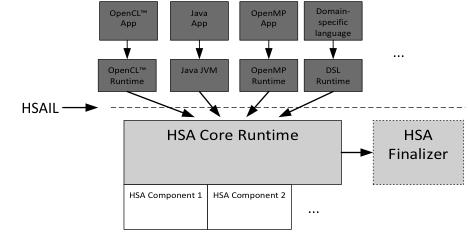
\includegraphics[width=0.5\textwidth]{fig/swarch}
  \centering
  \caption{HSA Software Architecture}
  \label{fig:swarch}
\end{figure}

Figure~\ref{fig:swarch} shows how the HSA Core Runtime fits into a
typical software architecture stack.

At the top of the stack is a programming model such as OpenCL™,
Java, OpenMP, or a domain-specific language (DSL).   The programming
model must include some way to indicate a parallel region that can
be accelerated.  For example, OpenCL has calls to
\texttt{clEnqueueNDRangeKernel} with associated kernels and grid ranges.
Java has the stream and lambda APIs, which provide support for both
multi-core CPUs and HSA Components.  OpenMP contains OMP pragmas
that mark parallel for loops and control other aspects of the
parallel implementation.  Other programming models can also build on
this same infrastructure.

The language compiler is responsible for generating HSAIL code for
the parallel regions.  HSA supports several options for when HSAIL
is generated and finalized.  One possibility is that the HSAIL is
generated by a high-level compiler and then embedded in the
application binary.  In this case, the finalizer is run when the
application loads and will convert the HSAIL to machine code for the
target machine.   Another option is that the HSAIL is finalized when
the applications is built, or the machine cod  The HSA Finalizer is
an optional component of the HSA Core Runtime, which may reduce the
footprint of the HSA software on systems where the finalization is
done before runtime.

Each language also includes a “language runtime” that connects the
language implementation to the HSA Core Runtime.   When the language
compiler generates code for a parallel region, it will include calls
to the HSA Runtime to set up and dispatch the work to the HSA
Component.   The language runtime is also responsible for
initializing HSA, and may utilize other HSA core runtime features as
well.

The API for the HSA core runtime is standard across all HSA vendors,
such that languages which use the HSA runtime can run on the
different vendors that support the API.  Each vendor is responsible
for supplying their own implementation which supports the hsa
component(s) in the vendor’s platform.   HSA does not provide a
mechanism to combine runtimes from different vendors; instead
vendors must provide a single runtime which supports all the
components in the platform.
The implementation of the HSA Runtime may include kernel-level
components (typical for hardware components) or may be entirely
user-space (simulators or CPU implementations).

\hypertarget{glue}{}\section{ Infrastructure and Execution
Flow}\label{glue}

\diffblock{
\hypertarget{executionmodel}{}\section{Execution
Model}\label{executionmodel}
}
\DIFdelbegin \DIFdel{Host/HSAIL – brief intro that describes host running host code
include HSA runtime, components running HSAIL.
}\DIFdelend

\diffblock{\hypertarget{archdispatch}{}\subsection{Architected Dispatch}
\label{archdispatch}}
Core runtime exposes several details of the HSA hardware,
including architected dispatches and support for execution control.
The overall goal of the core runtime design is to provide a
high-\/performance dispatch mechanism that is portable across
multiple H\-S\-A vendor architectures. Two vendors with the same
host I\-S\-A but different H\-S\-A-\/compliant G\-P\-Us will be able
to run the same unmodified binary, because they support the
H\-S\-A-\/architected A\-Q\-L interface and supply a library
that implements the architected core runtime A\-P\-I.

In order for user-level applications to use the HSA system and HSA
components, they need to write HSAIL programs and compile and
execute these programs using user mode queues and AQL commands.  The
HSA Programmer’s Reference Manual (PRM) defines HSAIL Virtual ISA
and Programming Model, serves as a Compiler Writer’s Guide, and
defines Object Format (BRIG). The HSA runtime helps setup the
execution via API calls and data structures to support architected
features.

The HSA core runtime realizes architected dispatch. Architected
dispatch is the key feature in an HSA system that enables a
user-\/level application to directly issue commands to the HSA
Component hardware.  Architected dispatch differentiates it from
other higher-\/level runtime systems and programming models\-: other
runtime systems provide software A\-P\-Is for setting arguments and
launching kernels, while H\-S\-A architects these at the hardware
and specification level.  The critical path of the dispatch
mechanism is architected at the H\-S\-A hardware level and can be
done with regular memory operations and runtime provided wrapper
API.  Fundamentally, the user creates user mode queues and an
A\-Q\-L Packet in memory, and then signals the HSA component to
begin executing the packet using light weight operations (which may
be wrapped with A\-P\-I calls).

This section describes various features core runtime provides to
support architected dispatch as steps that a user needs to take to
utilize runtime.

\subsection{Initial Setup}
One of the first steps in the setup is that of device discovery.
Device discovery is performed at the initialization of the core
runtime and information is made available to the user as data
structures. Section~\ref{topology} describes these structures.
The next step in the setup is creation of the
component queues. Queues are an HSA architected mechanism to submit
work to the HSA component HW. The interfaces for queue creation
are defined in Section~\ref{architected_queue}. Different
components may provide
implementation-\/specific code under the core A\-P\-I for these
functions. H\-S\-A runtime also includes mechanisms to provide
implementation-\/specific data as part of the dispatch, provided
such data can be computed at compile time.

\subsection{Compilation Flow}
Once an HSAIL program is written or generated by a higher-level
compilation step, it needs to be \emph{assembled} to generate a
BRIG. BRIG is the HSAIL object format and is specified in the PRM.
HSA runtime defines API call to compile the BRIG and generate a code
object that has sufficient information to execute the user
program. The details of this compilation process and symbol
resolution are discussed in Section~\ref{finalizerchapter}.

\subsection{Execution of Kernel}
The Systems Architecture Requirements (SAR) document specifies the
structure of the \emph{packets} (i.e. commands) that can be placed on
the HSA user mode queues for the component HW to execute them. The
format of the packets is architected and they are referred to as
Architected Queuing Language (AQL) packets. One of the types of AQL
packets is a dispatch AQL packet.
The user can now create an AQL packet
and initialize it with the code object obtained from the
finalization step, including the
allocation of memory to hold the kernel arguments and the
spill/arg/private memory.
The interface for kernel arguments between the runtime and the
kernel I\-S\-A (instruction set architecture) is also architected at
the H\-S\-A level. This is covered in the H\-S\-A\-I\-L A\-B\-I
(this is discussed in
Section~\ref{coreapi_HSAIL_ABI}),
which specifies the in-\/memory layout of the kernarg segment. Users
can determine the layout of the kernarg memory segment at compile
time merely by examining the signature of the H\-S\-A\-I\-L
function. The finalizer is required to support this A\-B\-I and thus
there is no need for runtime metadata to specify the position or
format of arguments.
This step can be done once for each A\-Q\-L packet creation.

Optimized implementations can cache the
result of this step and re-\/use the A\-Q\-L packet for subsequent
launches. Care must be taken to ensure that the A\-Q\-L Dispatch
packet (and the associated kernel and spill/arg/private memory) is
not re-\/used before the launch completes. For simple cases, (that
is, a single-\/thread, synchronous launch, the
AQL dispatch packet(s) can be declared as a static variable
and initialized at the same time the code is finalized. More
advanced cases can create and track several
AQL Dispatch packet(s) for a single kernel code object.

HSA HW defines a packet process for processing these packets and a doorbell
mechanism to inform the packet processing HW that packets have been
written into the queue. The Core runtime defines a structure and update
API to inform the HW that the dispatch packet has been written to the
queue. Different packet formats and states of a packet are discussed
in Section~\ref{AQL}. Section~\ref{architected_queue} discusses the
queue creation and various states the queue can be in, once it is
created.

Once the packet is written and the HW is informed by way of the
doorbell, the execution can start. The execution happens
asynchronously. The user is free to write more packets for executing
other kernels in the queue. This activity can overlap the actual
execution of the kernel.

\subsection{Determining Kernel Completion}
HSA SAR defines signals as a mechanism for communication between
different parts of a HSA system. Signals are defined as opaque
objects in the HSA core runtime and APIs have been defined to send a
value to the signal and wait for a value at the signal,
Section~\ref{signals} discusses signals in detail. The AQL dispatch
packet has a provision for the user to pass in an opaque signal.
When the HSA Component HW observes a valid signal in the AQL packet,
it sends a value to this signal when execution of the kernel is
complete (success or error). The user can wait on this signal to
determine kernel completion. Errors and their
meaning are discussed in Section~\ref{error}.
\begin{framed}
\lstinputlisting{example/main.c}
\end{framed}

\hypertarget{index_overview}{}\section{Overview}\label{index_overview}

Recent system-on-a-chip designs have integrated CPU, GPU, and other
accelerator devices onto a single chip with a shared high-bandwidth
memory system.  In fact, these single-chip designs are now widely
used in many computing markets including cellphones, tablets,
personal computers, and game consoles. The Heterogeneous System
Architecture (HSA) builds on the close physical integration of
accelerators that is already occurring in the marketplace, and takes
the next step by defining standards for uniting the accelerators
architecturally.  The HSA specifications includes requirements for
virtual memory, memory coherency, architected dispatch mechanisms,
and power-efficient signals.
HSA refers to these accelerators as “components”.  The system
architecture defines a consistent base for building portable
applications that access the power and performance benefits of the
dedicated hsa components.   Many of these components, including GPUs
and DSPs, are capable and flexible processors that have been
extended with special hardware for accelerating parallel code.
Historically these devices have been difficult to program due to a
need for specialized or proprietary programming languages.  HSA aims
to bring the benefits of these components to mainstream programming
languages using similar or identical syntax to that which is
provided for accessing multi-core CPUs.

In addition to the system architecture, HSA’s “Programmer’s
Reference Guide” defines HSAIL - a portable, low-level, compiler
intermediate language designed for parallel computing.

\begin{description}
\item[Portable:] The HSAIL language is an open-standard, supported by
multiple vendors in the HSA Foundation, and is portable across
vendors and product generations, so that applications which use
HSAIL are guaranteed to run on future hardware that supports the
HSAIL standard.
\item[Low-level:] HSAIL’s representation is just above the machine
instruction set.  Most optimizations including register allocation
are intended to be performed by the compiler that generates HSAIL.
HSAIL code is translated to the host instruction set by a tool
called the “finalizer”.  Each component will provide its own
implementation of the finalizer.  The finalization step is intended
to be lightweight, fast, and simple.  Importantly, the finalizer
step does not involve a complex compiler.  Applications which
contain HSAIL should not see different functional or performance
behavior from new finalizer versions that might be deployed in the
field after the application ships.
\item[Designed for parallel computing:] HSAIL is intended to represent
the parallel sections of an application.  It complements but does
not replace the host code – host code still exists and is used for
the serial portion of the application.  HSAIL represents a single
“lane” of execution, and the parallelism is expressed in the grid
dimensions that are specified when the HSAIL kernel is dispatched to
a target component.  In this way, HSAIL does not encode a specific
“vector width” and can be used to represent a variety of different
parallel computing devices.
\end{description}

For more information on HSAIL, refer to the HSA Programmer’s
Reference Guide.

The final piece of the puzzle is the HSA Core Runtime API.  The core
runtime is a thin, user-mode API that provides the interfaces
necessary for the host to launch compute kernels to the available
components.  This document describes the architecture and APIs for
the HSA Core Runtime.  Key sections of the runtime API include:

\begin{itemize}
\item Error handling
\item Runtime initialization (open/close)
\item Topology and Component Discovery
\item Signals and Synchronization
\item Architected Dispatch
\item Memory Management
\end{itemize}

In summary, there are three specifications provided by the HSA
Foundation:
\begin{description}
\item[HSA System Architecture Requirements:] Architectural foundation for
how HSA components share memory and communicate work requests.
\item[HSA Programmer’s Reference Manual:] Describes HSAIL, a low-level,
portable compiler IR appropriate for use as compiler intermediate
language.
\item[HSA Runtime Specification:] This document.  Describes the host-side
API for controlling the launch of HSAIL kernels.
\end{description}

The remainder of this document describes the HSA software
architecture and execution model, and includes functional
descriptions for all of the HSA APIs and associated data structures.

\begin{figure}
  \centering
  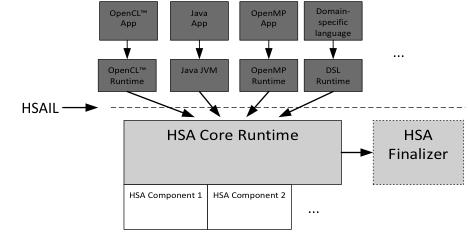
\includegraphics[width=0.5\textwidth]{fig/swarch}
  \centering
  \caption{HSA Software Architecture}
  \label{fig:swarch}
\end{figure}

Figure~\ref{fig:swarch} shows how the HSA Core Runtime fits into a
typical software architecture stack.

At the top of the stack is a programming model such as OpenCL™,
Java, OpenMP, or a domain-specific language (DSL).   The programming
model must include some way to indicate a parallel region that can
be accelerated.  For example, OpenCL has calls to
\texttt{clEnqueueNDRangeKernel} with associated kernels and grid ranges.
Java has the stream and lambda APIs, which provide support for both
multi-core CPUs and HSA Components.  OpenMP contains OMP pragmas
that mark parallel for loops and control other aspects of the
parallel implementation.  Other programming models can also build on
this same infrastructure.

The language compiler is responsible for generating HSAIL code for
the parallel regions.  HSA supports several options for when HSAIL
is generated and finalized.  One possibility is that the HSAIL is
generated by a high-level compiler and then embedded in the
application binary.  In this case, the finalizer is run when the
application loads and will convert the HSAIL to machine code for the
target machine.   Another option is that the HSAIL is finalized when
the applications is built, or the machine cod  The HSA Finalizer is
an optional component of the HSA Core Runtime, which may reduce the
footprint of the HSA software on systems where the finalization is
done before runtime.

Each language also includes a “language runtime” that connects the
language implementation to the HSA Core Runtime.   When the language
compiler generates code for a parallel region, it will include calls
to the HSA Runtime to set up and dispatch the work to the HSA
Component.   The language runtime is also responsible for
initializing HSA, and may utilize other HSA core runtime features as
well.

The API for the HSA core runtime is standard across all HSA vendors,
such that languages which use the HSA runtime can run on the
different vendors that support the API.  Each vendor is responsible
for supplying their own implementation which supports the hsa
component(s) in the vendor’s platform.   HSA does not provide a
mechanism to combine runtimes from different vendors; instead
vendors must provide a single runtime which supports all the
components in the platform.
The implementation of the HSA Runtime may include kernel-level
components (typical for hardware components) or may be entirely
user-space (simulators or CPU implementations).

\hypertarget{glue}{}\section{ Infrastructure and Execution
Flow}\label{glue}

\diffblock{
\hypertarget{executionmodel}{}\section{Execution
Model}\label{executionmodel}
}
\diffblock{\hypertarget{archdispatch}{}\subsection{Architected Dispatch}
\label{archdispatch}}
Core runtime exposes several details of the HSA hardware,
including architected dispatches and support for execution control.
The overall goal of the core runtime design is to provide a
high-\/performance dispatch mechanism that is portable across
multiple H\-S\-A vendor architectures. Two vendors with the same
host I\-S\-A but different H\-S\-A-\/compliant G\-P\-Us will be able
to run the same unmodified binary, because they support the
H\-S\-A-\/architected A\-Q\-L interface and supply a library
that implements the architected core runtime A\-P\-I.

In order for user-level applications to use the HSA system and HSA
components, they need to write HSAIL programs and compile and
execute these programs using user mode queues and AQL commands.  The
HSA Programmer’s Reference Manual (PRM) defines HSAIL Virtual ISA
and Programming Model, serves as a Compiler Writer’s Guide, and
defines Object Format (BRIG). The HSA runtime helps setup the
execution via API calls and data structures to support architected
features.

The HSA core runtime realizes architected dispatch. Architected
dispatch is the key feature in an HSA system that enables a
user-\/level application to directly issue commands to the HSA
Component hardware.  Architected dispatch differentiates it from
other higher-\/level runtime systems and programming models\-: other
runtime systems provide software A\-P\-Is for setting arguments and
launching kernels, while H\-S\-A architects these at the hardware
and specification level.  The critical path of the dispatch
mechanism is architected at the H\-S\-A hardware level and can be
done with regular memory operations and runtime provided wrapper
API.  Fundamentally, the user creates user mode queues and an
A\-Q\-L Packet in memory, and then signals the HSA component to
begin executing the packet using light weight operations (which may
be wrapped with A\-P\-I calls).

This section describes various features core runtime provides to
support architected dispatch as steps that a user needs to take to
utilize runtime.

\subsection{Initial Setup}
One of the first steps in the setup is that of device discovery.
Device discovery is performed at the initialization of the core
runtime and information is made available to the user as data
structures. Section~\ref{topology} describes these structures.
The next step in the setup is creation of the
component queues. Queues are an HSA architected mechanism to submit
work to the HSA component HW. The interfaces for queue creation
are defined in Section~\ref{architected_queue}. Different
components may provide
implementation-\/specific code under the core A\-P\-I for these
functions. H\-S\-A runtime also includes mechanisms to provide
implementation-\/specific data as part of the dispatch, provided
such data can be computed at compile time.

\subsection{Compilation Flow}
Once an HSAIL program is written or generated by a higher-level
compilation step, it needs to be \emph{assembled} to generate a
BRIG. BRIG is the HSAIL object format and is specified in the PRM.
HSA runtime defines API call to compile the BRIG and generate a code
object that has sufficient information to execute the user
program. The details of this compilation process and symbol
resolution are discussed in Section~\ref{finalizerchapter}.

\subsection{Execution of Kernel}
The Systems Architecture Requirements (SAR) document specifies the
structure of the \emph{packets} (i.e. commands) that can be placed on
the HSA user mode queues for the component HW to execute them. The
format of the packets is architected and they are referred to as
Architected Queuing Language (AQL) packets. One of the types of AQL
packets is a dispatch AQL packet.
The user can now create an AQL packet
and initialize it with the code object obtained from the
finalization step, including the
allocation of memory to hold the kernel arguments and the
spill/arg/private memory.
The interface for kernel arguments between the runtime and the
kernel I\-S\-A (instruction set architecture) is also architected at
the H\-S\-A level. This is covered in the H\-S\-A\-I\-L A\-B\-I
(this is discussed in
Section~\ref{coreapi_HSAIL_ABI}),
which specifies the in-\/memory layout of the kernarg segment. Users
can determine the layout of the kernarg memory segment at compile
time merely by examining the signature of the H\-S\-A\-I\-L
function. The finalizer is required to support this A\-B\-I and thus
there is no need for runtime metadata to specify the position or
format of arguments.
This step can be done once for each A\-Q\-L packet creation.

Optimized implementations can cache the
result of this step and re-\/use the A\-Q\-L packet for subsequent
launches. Care must be taken to ensure that the A\-Q\-L Dispatch
packet (and the associated kernel and spill/arg/private memory) is
not re-\/used before the launch completes. For simple cases, (that
is, a single-\/thread, synchronous launch, the
AQL dispatch packet(s) can be declared as a static variable
and initialized at the same time the code is finalized. More
advanced cases can create and track several
AQL Dispatch packet(s) for a single kernel code object.

HSA HW defines a packet process for processing these packets and a doorbell
mechanism to inform the packet processing HW that packets have been
written into the queue. The Core runtime defines a structure and update
API to inform the HW that the dispatch packet has been written to the
queue. Different packet formats and states of a packet are discussed
in Section~\ref{AQL}. Section~\ref{architected_queue} discusses the
queue creation and various states the queue can be in, once it is
created.

Once the packet is written and the HW is informed by way of the
doorbell, the execution can start. The execution happens
asynchronously. The user is free to write more packets for executing
other kernels in the queue. This activity can overlap the actual
execution of the kernel.

\subsection{Determining Kernel Completion}
HSA SAR defines signals as a mechanism for communication between
different parts of a HSA system. Signals are defined as opaque
objects in the HSA core runtime and APIs have been defined to send a
value to the signal and wait for a value at the signal,
Section~\ref{signals} discusses signals in detail. The AQL dispatch
packet has a provision for the user to pass in an opaque signal.
When the HSA Component HW observes a valid signal in the AQL packet,
it sends a value to this signal when execution of the kernel is
complete (success or error). The user can wait on this signal to
determine kernel completion. Errors and their
meaning are discussed in Section~\ref{error}.
\begin{framed}
\lstinputlisting{example/main.c}
\end{framed}

\chapter{HSA Core A\-P\-I Specification and Description} \label{coreapi}
\hypertarget{coreapi}{}
This chapter describes HSA Core runtime API by their functional
area. Note that except for any setter/getter API, the remainder of
the core runtime API may be considered thread-safe.  Both the signal
update and the queue index update API are setter/getter API and
define scope an synchronization that applies to the updates and
operate on structure elements.

Several operating systems allow functions to be executed when a DLL
or a shared library is loaded (e.g. DLL main in Windows and GCC
\emph{constructor/destructor} attributes that allow functions to be
executed prior to main in several operating systems).
Whether or not the HSA runtime functions are allowed to be invoked
in such fashion may be implementation specific and are outside the
scope of this specification.

Similarly, any header files distributed by the HSA foundation for
this spec may contain calling convention specific prefixes such as
\_\_cdecl or \_\_stdcall. Such calling conventions are again invocation,
usage and implementation specific. Hence, the calling convention
specific prefix definition is outside the scope of API definition.

%%\begin{DIFnomarkup}
\hypertarget{error}{}\section{Synchronous and Asynchronous Errors and
Asynchronous Notification}
\label{error}
\end{DIFnomarkup}

Error handling in the core runtime can broadly be classified into
two categories: synchronous error handling and asynchronous
error/notification handling.

Synchronous errors are always reported when the call returns. They
indicate if the API returned a success or an error.

Asynchronous errors can occur due to various reasons:
\begin{inparaenum}[(i)]

\item Activity in packet processor, executing kernels, their actions
and memory accesses. If an error is detected during execution of a
kernel, the completion signal (if present) will be signaled with an
error indication value.

\item To provide \emphld{information/warning} (not as an exception
in expected behavior but by definition). This information/warning
may not necessarily indicate an error. For example, a timeout may be
an acceptable response for a wait API but is not indicative of a
failure.

\end{inparaenum}

\begin{DIFnomarkup}
\hypertarget{syncerror}{}\subsection{Synchronous Errors }\label{syncerror}
\end{DIFnomarkup}

When a core runtime API is called by the user and does not execute
successfully, the core runtime returns a status that can help
determine a cause of the unsuccessful execution. Each API call
discussed in this chapter defines what constitutes a successful
execution. While a few error conditions can be generalized to a
certain degree (e.g. failure in allocating system memory) many
errors can have system/implementation specific explanations.

The HSA core runtime API defines an enumeration that captures the
result of any API function that has been executed (the only
exception to this behavior are setter/getter API that access core
runtime structures). This enumeration is of the type
\dbtt{hsa\_status\_t} and enumerates \emphld{success},
\emphld{info}, and \emphld{error}. The \emphld{info} status definition
is discussed in Section ~\ref{asyncerror}.

\emphld{Success} status is a single value,
\dbtt{HSA\_STATUS\_SUCCESS}. Description of every core runtime
API call that returns \dbtt{hsa\_status\_t} explains the
expected successful behavior for that API. The value of
\dbtt{HSA\_STATUS\_SUCCESS} is always 0.

\emphld{Error} status could be due to user input/actions that are not
allowed (e.g. negative value in a size for allocation) or systemic
errors (e.g. an asynchronous activity lead to a failure that
cascaded into a failure in this API). The constants used for error
status are restricted to the negative range of values within the
\dbtt{hsa\_status\_t} enumeration. Errors must always have a
negative value. The Name of any constant that indicates an error status is
prefixed by \dbtt{HSA\_STATUS\_ERROR}. Errors could potentially be
implementation.

While the name of the constant in itself is informative for success,
info or error status, there may be scenarios where
\begin{inparaenum}[(i)] \item the user may request more information
about the meaning of a particular status, or, \item the return
status was implementation specific and the user needs to decode it.
\end{inparaenum} In the case of implementation specific status, the
negative number returned for error may not correspond to a
particular enumeration constant. To query additional
information on synchronous errors, the core runtime defines the
following API:

\input{example/APIhsa_status_query}

This API returns \dbtt{HSA\_STATUS\_SUCCESS} if one or both of the
{\itshape status\_info} and {\itshape status\_info\_string} have been
successfully updated with information regarding the input
{\itshape input\_status}. Otherwise it returns one of the following errors:

\begin{easylist}
& \dbtt{HSA\_STATUS\_NONE} when no additional information is
available regarding the status user requested.
& \dbtt{HSA\_STATUS\_ERROR\_INVALID\_ARGUMENT} if a NULL value is
passed for either of the arguments
\end{easylist}

\begin{DIFnomarkup}
\hypertarget{asyncerror}{}\subsection{Asynchronous Errors and
Notifications}\label{asyncerror}
\end{DIFnomarkup}

The HSA core runtime supports user-defined callbacks to handle
asynchronous errors. There are two different categories of callbacks
that can be registered by the user: \begin{inparaenum}[(i)] \item
for asynchronous information or warnings generated when the runtime
is executing, or, \item for asynchronous errors that get generated
in packet processor, or while executing a kernel \end{inparaenum}.
The core runtime supports a callback each for asynchronous errors
and notifications.
The user must use caution when using blocking functions within their
callback implementation -- a callback that does not return can
render the runtime state to be undefined. The user cannot depend on
thread local storage within the callbacks implementation and may
safely kill the thread that registers the callback. It is the user's
responsibility to ensure that the callback function is thread-safe.
The runtime does not implement any default callbacks.

\subsubsection{Asynchronous Notification of Information or
Warning}\label{asynnotif}

The information/warning status is represented by a value greater
than 0 within the \dbtt{hsa\_status\_t} enumeration. The status is
up to user interpretation and the runtime allows the user to
register a callback to take necessary action. Consider the example
where a user calls the initialize API to initialize the core runtime
and the return status is
\dbtt{HSA\_STATUS\_INFO\_ALREADY\_INITIALIZED} (to indicate that
the core runtime has already been initialized). This result may be
interpreted differently in different usage scenarios. A callback for
such notifications may be registered via \ttbf{hsa\_open} API
discussed in Section~\ref{init} or via
\ttbf{hsa\_notification\_callback\_register} API, which is defined
as follows:

\input{example/APIregister_notify}

The {\itshape context} parameter is used to identify a particular
runtime context that this callback is registered for. When a
callback is registered for a particular context, it will only be
invoked if the notification is for an action in that context.
Section~\ref{init} discusses the context in detail. The
\ttbf{hsa\_notification\_callback\_register} API can return one of
the following errors:
\begin{easylist}
& \dbtt{HSA\_STATUS\_ERROR\_OUT\_OF\_RESOURCES} if there is a failure
in allocation of an internal structure required by the core runtime
library in the context of registering a callback. This error may
also occur when the core runtime library needs to spawn threads or
create internal OS-specific events.
& \dbtt{HSA\_STATUS\_ERROR\_INVALID\_ARGUMENT}
if {\itshape info} is NULL.
@ \dbtt{HSA\_STATUS\_INVALID\_CONTEXT} if the context is invalid
(e.g. referenced counted to 0).
\end{easylist}

One of the arguments of the notification callback is a structure
that contains notification information. The structure is defined as
follows:

\input{example/STRnotify_message}

\subsubsection{Asynchronous Notification of Errors}\label{asynnotif}

The HSA system can have several queues in operation and
several kernels executing from these queues asynchronously.
When any asynchronous activity generates an error, the action that
initiated the activity may have concluded. To deal with
asynchronous errors, the core runtime supports asynchronous error
callbacks. The asynchronous error callback may be registered by means of the
\ttbf{hsa\_open} API discussed in Section~\ref{init} or via
\ttbf{hsa\_error\_callback\_register} API, which is defined as
follows:

\input{example/APIregister_error}

Details on how association of the callback can be done with
asynchronous activities are discussed in Sections~\ref{init} and
\ref{architected_queue}. The {\itshape context} parameter is used
to identify a particular runtime context that this callback is
registered for. When a callback is registered for a particular
context, it will only be invoked if the notification is for an
action in that context. For example, if a queue was created for a
runtime context {\itshape c1} and a callback registered for a
context {\itshape c2} but not for {\itshape c1}, any error on the
queue, such as a packet processing error, will not trigger the
execution of asynchronous error callback registered for context
{\itshape c1}. This API can return one of the following errors:

\begin{easylist}
& \dbtt{HSA\_STATUS\_ERROR\_OUT\_OF\_RESOURCES} if there is a failure
in allocation of an internal structure required by the core runtime
library in the context of registering a callback. This error may
also occur when the core runtime library needs to spawn threads or
create internal OS-specific events.
& \dbtt{HSA\_STATUS\_ERROR\_INVALID\_ARGUMENT}
if {\itshape info} is NULL.
\end{easylist}

One of the arguments of the notification callback is a structure
that contains notification information. The structure is defined as
follows:

\input{example/STRerror_message}

\subsection{Asynchronous Notification Example}
\lstinputlisting{example/asyncerror.c}


\begin{DIFnomarkup}
\hypertarget{error}{}\section{Synchronous and Asynchronous Errors and
Asynchronous Notification}
\label{error}
\end{DIFnomarkup}

Error handling in the core runtime can broadly be classified into
two categories: synchronous error handling and asynchronous
error/notification handling.

Synchronous errors are always reported when the call returns. They
indicate if the API returned a success or an error.

Asynchronous errors can occur due to various reasons:
\begin{inparaenum}[(i)]

\item Activity in packet processor, executing kernels, their actions
and memory accesses. If an error is detected during execution of a
kernel, the completion signal (if present) will be signaled with an
error indication value.

\item To provide \emphld{information/warning} (not as an exception
in expected behavior but by definition). This information/warning
may not necessarily indicate an error. For example, a timeout may be
an acceptable response for a wait API but is not indicative of a
failure.

\end{inparaenum}

\begin{DIFnomarkup}
\hypertarget{syncerror}{}\subsection{Synchronous Errors }\label{syncerror}
\end{DIFnomarkup}

When a core runtime API is called by the user and does not execute
successfully, the core runtime returns a status that can help
determine a cause of the unsuccessful execution. Each API call
discussed in this chapter defines what constitutes a successful
execution. While a few error conditions can be generalized to a
certain degree (e.g. failure in allocating system memory) many
errors can have system/implementation specific explanations.

The HSA core runtime API defines an enumeration that captures the
result of any API function that has been executed (the only
exception to this behavior are setter/getter API that access core
runtime structures). This enumeration is of the type
\dbtt{hsa\_status\_t} and enumerates \emphld{success},
\emphld{info}, and \emphld{error}. The \emphld{info} status definition
is discussed in Section ~\ref{asyncerror}.

\emphld{Success} status is a single value,
\dbtt{HSA\_STATUS\_SUCCESS}. Description of every core runtime
API call that returns \dbtt{hsa\_status\_t} explains the
expected successful behavior for that API. The value of
\dbtt{HSA\_STATUS\_SUCCESS} is always 0.

\emphld{Error} status could be due to user input/actions that are not
allowed (e.g. negative value in a size for allocation) or systemic
errors (e.g. an asynchronous activity lead to a failure that
cascaded into a failure in this API). The constants used for error
status are restricted to the negative range of values within the
\dbtt{hsa\_status\_t} enumeration. Errors must always have a
negative value. The Name of any constant that indicates an error status is
prefixed by \dbtt{HSA\_STATUS\_ERROR}. Errors could potentially be
implementation.

While the name of the constant in itself is informative for success,
info or error status, there may be scenarios where
\begin{inparaenum}[(i)] \item the user may request more information
about the meaning of a particular status, or, \item the return
status was implementation specific and the user needs to decode it.
\end{inparaenum} In the case of implementation specific status, the
negative number returned for error may not correspond to a
particular enumeration constant. To query additional
information on synchronous errors, the core runtime defines the
following API:

\input{example/APIhsa_status_query}

This API returns \dbtt{HSA\_STATUS\_SUCCESS} if one or both of the
{\itshape status\_info} and {\itshape status\_info\_string} have been
successfully updated with information regarding the input
{\itshape input\_status}. Otherwise it returns one of the following errors:

\begin{easylist}
& \dbtt{HSA\_STATUS\_NONE} when no additional information is
available regarding the status user requested.
& \dbtt{HSA\_STATUS\_ERROR\_INVALID\_ARGUMENT} if a NULL value is
passed for either of the arguments
\end{easylist}

\begin{DIFnomarkup}
\hypertarget{asyncerror}{}\subsection{Asynchronous Errors and
Notifications}\label{asyncerror}
\end{DIFnomarkup}

The HSA core runtime supports user-defined callbacks to handle
asynchronous errors. There are two different categories of callbacks
that can be registered by the user: \begin{inparaenum}[(i)] \item
for asynchronous information or warnings generated when the runtime
is executing, or, \item for asynchronous errors that get generated
in packet processor, or while executing a kernel \end{inparaenum}.
The core runtime supports a callback each for asynchronous errors
and notifications.
The user must use caution when using blocking functions within their
callback implementation -- a callback that does not return can
render the runtime state to be undefined. The user cannot depend on
thread local storage within the callbacks implementation and may
safely kill the thread that registers the callback. It is the user's
responsibility to ensure that the callback function is thread-safe.
The runtime does not implement any default callbacks.

\subsubsection{Asynchronous Notification of Information or
Warning}\label{asynnotif}

The information/warning status is represented by a value greater
than 0 within the \dbtt{hsa\_status\_t} enumeration. The status is
up to user interpretation and the runtime allows the user to
register a callback to take necessary action. Consider the example
where a user calls the initialize API to initialize the core runtime
and the return status is
\dbtt{HSA\_STATUS\_INFO\_ALREADY\_INITIALIZED} (to indicate that
the core runtime has already been initialized). This result may be
interpreted differently in different usage scenarios. A callback for
such notifications may be registered via \ttbf{hsa\_open} API
discussed in Section~\ref{init} or via
\ttbf{hsa\_notification\_callback\_register} API, which is defined
as follows:

\input{example/APIregister_notify}

The {\itshape context} parameter is used to identify a particular
runtime context that this callback is registered for. When a
callback is registered for a particular context, it will only be
invoked if the notification is for an action in that context.
Section~\ref{init} discusses the context in detail. The
\ttbf{hsa\_notification\_callback\_register} API can return one of
the following errors:
\begin{easylist}
& \dbtt{HSA\_STATUS\_ERROR\_OUT\_OF\_RESOURCES} if there is a failure
in allocation of an internal structure required by the core runtime
library in the context of registering a callback. This error may
also occur when the core runtime library needs to spawn threads or
create internal OS-specific events.
& \dbtt{HSA\_STATUS\_ERROR\_INVALID\_ARGUMENT}
if {\itshape info} is NULL.
@ \dbtt{HSA\_STATUS\_INVALID\_CONTEXT} if the context is invalid
(e.g. referenced counted to 0).
\end{easylist}

One of the arguments of the notification callback is a structure
that contains notification information. The structure is defined as
follows:

\input{example/STRnotify_message}

\subsubsection{Asynchronous Notification of Errors}\label{asynnotif}

The HSA system can have several queues in operation and
several kernels executing from these queues asynchronously.
When any asynchronous activity generates an error, the action that
initiated the activity may have concluded. To deal with
asynchronous errors, the core runtime supports asynchronous error
callbacks. The asynchronous error callback may be registered by means of the
\ttbf{hsa\_open} API discussed in Section~\ref{init} or via
\ttbf{hsa\_error\_callback\_register} API, which is defined as
follows:

\input{example/APIregister_error}

Details on how association of the callback can be done with
asynchronous activities are discussed in Sections~\ref{init} and
\ref{architected_queue}. The {\itshape context} parameter is used
to identify a particular runtime context that this callback is
registered for. When a callback is registered for a particular
context, it will only be invoked if the notification is for an
action in that context. For example, if a queue was created for a
runtime context {\itshape c1} and a callback registered for a
context {\itshape c2} but not for {\itshape c1}, any error on the
queue, such as a packet processing error, will not trigger the
execution of asynchronous error callback registered for context
{\itshape c1}. This API can return one of the following errors:

\begin{easylist}
& \dbtt{HSA\_STATUS\_ERROR\_OUT\_OF\_RESOURCES} if there is a failure
in allocation of an internal structure required by the core runtime
library in the context of registering a callback. This error may
also occur when the core runtime library needs to spawn threads or
create internal OS-specific events.
& \dbtt{HSA\_STATUS\_ERROR\_INVALID\_ARGUMENT}
if {\itshape info} is NULL.
\end{easylist}

One of the arguments of the notification callback is a structure
that contains notification information. The structure is defined as
follows:

\input{example/STRerror_message}
\subsection{Asynchronous Notification Example}
\lstinputlisting{example/asyncerror.c}

%%\DIFdelbegin %DIFDELCMD < \begin{DIFnomarkup}
%DIFDELCMD < \hypertarget{init}{}\section{Open and close
%DIFDELCMD < API}\label{init}
%DIFDELCMD < \end{DIFnomarkup}
%DIFDELCMD < %%%
\DIFdelend \DIFaddbegin \begin{DIFnomarkup}
\hypertarget{init}{}\section{Open and close
}\label{init}
\end{DIFnomarkup}
\DIFaddend

Since HSA core runtime is a user mode library, its state is a part
of the application's process space. When the runtime is opened for
the first time, a runtime instance for that application process is
created. Closing a runtime destroys this instance. An application
may open (or close) the HSA runtime multiple times within the same
process and potentially within multiple threads -- only a
single instance of the runtime, per-process, will exist.

The core runtime defines a runtime context that acts as a reference
counting mechanism and a scheme to differentiate multiple usages of
the runtime within the same application process. The runtime context
is generated when the runtime is opened or when a
user calls the acquire API that is defined in this Section. As an
example, consider an application that is using the runtime but also
uses a library, this library also creates HSA queues and submits
work to them. Both the library and the application may want to register
callbacks, and to capture notifications/errors of their specific
usage. The runtime context helps identify the different usages (within
the same process) and channel errors and notifications to
appropriate callbacks. It also acts as a reference counting
mechanism; while correctly \emphld{acquired}, the runtime context
ensures that the runtime instance will not be shutdown until the
context is \emphld{released} (this, in effect, is the reference
counting part of the context).

This section defines four new API, \ttbf{hsa\_open} to open the
runtime instance, \ttbf{hsa\_close} to close it,
\ttbf{hsa\_context\_acquire} to create a new context (and increment
the reference count), and, \ttbf{hsa\_context\_release} to release
the acquired context (and decrement the reference count).

Invocation of \ttbf{hsa\_open} initializes the HSA runtime if it is
not already initialized. It is allowed for applications to invoke
\ttbf{hsa\_open} multiple times and do multiple \ttbf{hsa\_close}
API calls. The HSA open call returns a new context at every
invocation.  Reference counting is a mechanism that allows the
runtime to keep a count of the number of different usages of the
runtime API within the same application process. This ensures that
the runtime stays active until a \ttbf{hsa\_close} is called by the
user when the reference count represented by that runtime context is
1.

The definition of the \ttbf{hsa\_open} API is as follows:

\input{example/APIhsa_initialize}

The open API returns \dbtt{HSA\_STATUS\_SUCCESS} if the
initialization was successful. Otherwise it returns one of the
following errors:

\begin{easylist}
& \dbtt{HSA\_STATUS\_ERROR\_OUT\_OF\_RESOURCES} if there is a
failure in allocation of an internal structure required by the core
runtime library. This error may also occur when the core runtime
library needs to spawn threads or create internal OS-specific
events.

& \dbtt{HSA\_STATUS\_ERROR\_COMPONENT\_INITIALIZATION} if there
is a non-specific failure in initializing one of the components.

& \dbtt{HSA\_STATUS\_ERROR\_CONTEXT\_NULL} if the context pointer
passed by the user is NULL. User is required to pass in a memory
backed context pointer.
\end{easylist}

If the HSA runtime is already initialized, an asynchronous
notification is generated by the runtime and
\dbtt{HSA\_STATUS\_SUCCESS} is returned. If the user chooses to
capture this asynchronous notification, the user should define a
callback and associate it with the context returned by the
\ttbf{hsa\_open} call.  Each \ttbf{hsa\_open} call increments the
reference count before returning success.

The runtime defines \ttbf{hsa\_close} as the corresponding API call
to finalize the use of the runtime API. This API takes in a context
as input. This API updates the reference count for every
invocation. Once the reference count is 0, it proceeds to relinquish
any resources allocated for the runtime and closes the runtime
instance. It is possible in a multi-threaded scenario that one
thread is doing a close while the other is trying to acquire the
runtime context or do an open. The core runtime specification
defines that an acquire with an input context that represents a
closed runtime instance will fail. However, \ttbf{hsa\_open} can be
called to create a new instance of the runtime after it is closed.
The API for \ttbf{hsa\_close} is defined as follows:

\input{example/APIhsa_close}

The close API returns \dbtt{HSA\_STATUS\_SUCCESS} if the close
was successful. Otherwise, it returns one of the following errors:

\begin{easylist}
& \dbtt{HSA\_STATUS\_ERROR\_NOT\_INITIALIZED} if the close was
called (a) either before the runtime was initialized, or (b)
after it has already been successfully closed.

& \dbtt{HSA\_STATUS\_ERROR\_RESOURCE\_FREE} if some of the
resources consumed during initialization by the runtime could not be
freed.
\end{easylist}

If the close is called when the reference count is not 1, it is
still considered a succesful invocation of close, in that, the
\dbtt{HSA\_STATUS\_SUCCESS} is returned with status
\dbtt{HSA\_STATUS\_CLOSE\_CONTEXT\_ACTIVE}, is generated by the
runtime on the context that is till active before the API returns.

The HSA core runtime API for an acquire on a context,
\ttbf{hsa\_context\_acquire}, is defined as follows:

\input{example/APIacquire_context}

The open API returns \dbtt{HSA\_STATUS\_SUCCESS} if the acquire was
successful and if {\itshape output\_context} holds the new context
generated. Otherwise it returns one of the following errors:

\begin{easylist}
& \dbtt{HSA\_STATUS\_ERROR\_NOT\_INITIALIZED} if the
\ttbf{hsa\_acquire\_context} was called (a) either before the
runtime was initialized, or (b) after it has already been
closed.
& \dbtt{HSA\_STATUS\_CONTEXT\_LIMIT\_REACHED} if the increment has
taken the context to the UINT64\_MAX value defined in
\texttt{stdint.h} C header file.
\end{easylist}

The corresponding release API, \ttbf{hsa\_context\_release} is
defined as follows:

\input{example/APIrelease_context}

The \ttbf{hsa\_context\_release} API returns
\dbtt{HSA\_STATUS\_SUCCESS} if the release was successful.
Otherwise it returns the following error:

\begin{easylist}
& \dbtt{HSA\_STATUS\_ERROR\_NOT\_INITIALIZED} if the
\ttbf{hsa\_release\_context} was called before the
runtime, after reference count has reached a value of 0.

Runtime context cannot be incremented beyond a 64bit unsigned
integer. The context does not wrap around.

\end{easylist}
\subsection{Open/Close Example}

\lstinputlisting{example/openclose.c}


\hypertarget{init}{}\section{Open and close}\label{init}

Since HSA core runtime is a user mode library, its state is a part
of the application's process space. When the runtime is opened for
the first time, a runtime instance for that application process is
created. Closing a runtime destroys this instance. An application
may open (or close) the HSA runtime multiple times within the same
process and potentially within multiple threads -- only a
single instance of the runtime, per-process, will exist.

The core runtime defines a runtime context that acts as a reference
counting mechanism and a scheme to differentiate multiple usages of
the runtime within the same application process. The runtime context
is generated when the runtime is opened or when a
user calls the acquire API that is defined in this Section. As an
example, consider an application that is using the runtime but also
uses a library, this library also creates HSA queues and submits
work to them. Both the library and the application may want to register
callbacks, and to capture notifications/errors of their specific
usage. The runtime context helps identify the different usages (within
the same process) and channel errors and notifications to
appropriate callbacks. It also acts as a reference counting
mechanism; while correctly \emphld{acquired}, the runtime context
ensures that the runtime instance will not be shutdown until the
context is \emphld{released} (this, in effect, is the reference
counting part of the context).

This section defines four new API, \ttbf{hsa\_open} to open the
runtime instance, \ttbf{hsa\_close} to close it,
\ttbf{hsa\_context\_acquire} to create a new context (and increment
the reference count), and, \ttbf{hsa\_context\_release} to release
the acquired context (and decrement the reference count).

Invocation of \ttbf{hsa\_open} initializes the HSA runtime if it is
not already initialized. It is allowed for applications to invoke
\ttbf{hsa\_open} multiple times and do multiple \ttbf{hsa\_close}
API calls. The HSA open call returns a new context at every
invocation.  Reference counting is a mechanism that allows the
runtime to keep a count of the number of different usages of the
runtime API within the same application process. This ensures that
the runtime stays active until a \ttbf{hsa\_close} is called by the
user when the reference count represented by that runtime context is
1.

The definition of the \ttbf{hsa\_open} API is as follows:

\input{example/APIhsa_initialize}

The open API returns \dbtt{HSA\_STATUS\_SUCCESS} if the
initialization was successful. Otherwise it returns one of the
following errors:

\begin{easylist}
& \dbtt{HSA\_STATUS\_ERROR\_OUT\_OF\_RESOURCES} if there is a
failure in allocation of an internal structure required by the core
runtime library. This error may also occur when the core runtime
library needs to spawn threads or create internal OS-specific
events.

& \dbtt{HSA\_STATUS\_ERROR\_COMPONENT\_INITIALIZATION} if there
is a non-specific failure in initializing one of the components.

& \dbtt{HSA\_STATUS\_ERROR\_CONTEXT\_NULL} if the context pointer
passed by the user is NULL. User is required to pass in a memory
backed context pointer.
\end{easylist}

If the HSA runtime is already initialized, an asynchronous
notification is generated by the runtime and
\dbtt{HSA\_STATUS\_SUCCESS} is returned. If the user chooses to
capture this asynchronous notification, the user should define a
callback and associate it with the context returned by the
\ttbf{hsa\_open} call.  Each \ttbf{hsa\_open} call increments the
reference count before returning success.

The runtime defines \ttbf{hsa\_close} as the corresponding API call
to finalize the use of the runtime API. This API takes in a context
as input. This API updates the reference count for every
invocation. Once the reference count is 0, it proceeds to relinquish
any resources allocated for the runtime and closes the runtime
instance. It is possible in a multi-threaded scenario that one
thread is doing a close while the other is trying to acquire the
runtime context or do an open. The core runtime specification
defines that an acquire with an input context that represents a
closed runtime instance will fail. However, \ttbf{hsa\_open} can be
called to create a new instance of the runtime after it is closed.
The API for \ttbf{hsa\_close} is defined as follows:

\input{example/APIhsa_close}

The close API returns \dbtt{HSA\_STATUS\_SUCCESS} if the close
was successful. Otherwise, it returns one of the following errors:

\begin{easylist}
& \dbtt{HSA\_STATUS\_ERROR\_NOT\_INITIALIZED} if the close was
called (a) either before the runtime was initialized, or (b)
after it has already been successfully closed.

& \dbtt{HSA\_STATUS\_ERROR\_RESOURCE\_FREE} if some of the
resources consumed during initialization by the runtime could not be
freed.
\end{easylist}

If the close is called when the reference count is not 1, it is
still considered a succesful invocation of close, in that, the
\dbtt{HSA\_STATUS\_SUCCESS} is returned with status
\dbtt{HSA\_STATUS\_CLOSE\_CONTEXT\_ACTIVE}, is generated by the
runtime on the context that is till active before the API returns.

The HSA core runtime API for an acquire on a context,
\ttbf{hsa\_context\_acquire}, is defined as follows:

\input{example/APIacquire_context}

The open API returns \dbtt{HSA\_STATUS\_SUCCESS} if the acquire was
successful and if {\itshape output\_context} holds the new context
generated. Otherwise it returns one of the following errors:

\begin{easylist}
& \dbtt{HSA\_STATUS\_ERROR\_NOT\_INITIALIZED} if the
\ttbf{hsa\_acquire\_context} was called (a) either before the
runtime was initialized, or (b) after it has already been
closed.
& \dbtt{HSA\_STATUS\_CONTEXT\_LIMIT\_REACHED} if the increment has
taken the context to the UINT64\_MAX value defined in
\texttt{stdint.h} C header file.
\end{easylist}

The corresponding release API, \ttbf{hsa\_context\_release} is
defined as follows:

\input{example/APIrelease_context}

The \ttbf{hsa\_context\_release} API returns
\dbtt{HSA\_STATUS\_SUCCESS} if the release was successful.
Otherwise it returns the following error:

\begin{easylist}
& \dbtt{HSA\_STATUS\_ERROR\_NOT\_INITIALIZED} if the
\ttbf{hsa\_release\_context} was called before the
runtime, after reference count has reached a value of 0.

Runtime context cannot be incremented beyond a 64bit unsigned
integer. The context does not wrap around.

\end{easylist}
\subsection{Open/Close Example}

\lstinputlisting{example/openclose.c}

%%\hypertarget{component}{}\section{Topology and Component
}\label{topology}
HSA platform topology information is provided by the runtime by way of
data structures so user can gather details about how a HSA
system/platform exposed its architectural details such as
\DIFdelbegin \DIFdel{components, memory, caches and connectivity (platform topology
requirement is described in the SAR document)}\DIFdelend \DIFaddbegin \DIFadd{agents and memory}\DIFaddend . This information
could be utilized by the user in different ways including decisions
on where to execute a particular user task. Core runtime
specification defines the topology table data structure and other
data structures to represent topology hierarchy.  After the core
runtime is initialized with \ttbf{hsa\_open}, the user may create a
local copy of the topology information using the API
\ttbf{hsa\_topology\_table\_create}. The user can parse this table
representing the HSA system to gather details such as the number of
different HSA Components on the system with local access to a
particular set of memory resources. \DIFaddbegin \DIFadd{Topology table is designed to be
allocated in a block of contiguous memory.
}\DIFaddend

The \ttbf{hsa\_topology\_table\_create} API is defined as follows:

\input{example/APItopology_create}

The API returns \dbtt{HSA\_STATUS\_SUCCESS} if the table has been
successfully created and returned by way of the {\itshape header}. Otherwise,
it returns one of the following errors:

\begin{easylist}
& \dbtt{HSA\_STATUS\_ERROR\_INVALID\_ARGUMENT} if {\itshape header}
is NULL.

& \dbtt{HSA\_STATUS\_ERROR\_OUT\_OF\_RESOURCES} if there is a failure
in allocation of an internal structure required by the core runtime
or in the creation of table header or the actual table.
\end{easylist}

\begin{figure}
  \centering
  \includegraphics[width=0.5\textwidth]{fig/topologytable}
  \centering
  \caption{Structure of the Topology Table}
  \label{fig:topology_table}
\end{figure}

The table structure is shown in Figure~\ref{fig:topology_table}.
The first entity in the table is a table header. This is the output
of the \ttbf{hsa\_topology\_table\_create} API.
The table header is defined by the following structure:
\input{example/STRtopology_header}

The table header structure includes the platform structure (
\dbtt{hsa\_platform\_t}).  The platform information in the platform
structure includes size/offset-array pairs for HSA agents
(\dbtt{hsa\_agent\_t}), memory (\dbtt{hsa\_memory\_descriptor\_t}) and
cache (\dbtt{hsa\_cache\_descriptor\_t}).
HSA platform can have a hierarchical structure with multiple
components/agents and physical memories.  The
\dbtt{hsa\_platform\_t} structure also includes properties such as
the clock frequency that are common across the platform and also
links to various elements in the topology table (see Figure
\ref{fig:topology_table} ).

The platform structure is defined as follows:

\input{example/STRhsa_platform}

When no information is available for a particular element, the
corresponding {\itshape number\_ \textless element \textgreater s}
field is set to zero by the runtime in the platform structure.
Platform structure maps to the agents, cache and physical memory,
\DIFdelbegin \DIFdel{etc.}%DIFDELCMD < \, %%%
\DIFdelend in the topology table for all nodes in the platform.

The core runtime defines the following structure to represent cache:
\input{example/STRhsa_cache_descriptor}
The structure holds associativity, cache size, cache line size for
all levels of cache and the inclusive property for all but the
last level. Each cache in the HSA system has a unique cache ID
identifying it.

The memory descriptor structure represents a physical memory block
or region and includes elements to provide bandwidth \DIFaddbegin \DIFadd{(an
implementation may chose to return 0 in the }{\itshape
\DIFadd{peak}\_bandwidth\_mbps} \DIFadd{field if it cannot provide bandwidth)}\DIFaddend , interleave
characteristics and latency for accessing memory. Implementations
may choose not to provide memory bandwidth or latency information.
The memory descriptor structure is defined as follows:

\input{example/STRhsa_memory_descriptor}

The structure:
\input{example/STRhsa_segment}
can represent any combination of the 7 HSA segments, a single
bit for each segment.

The HSA Agent data structure represents an HSA component when the
{\itshape agent\_type} field in the agent structure is set to a 1
(i.e. bit 0 is set to 1).
The structure contains elements that describe its properties. Each
component has access to coherent global memory (the HSA global
segment, and as per the requirement defined in SAR, has access to
other segments as well). The {\itshape agent\_type} is utilized as a
bit-field. Setting bit 2 indicates that the agent is a host, bit 3
indicates that agent can participate in agent dispatches. All
three bits or a combination of them can be set by the HSA runtime.

The structure of the HSA agent/component is defined as follows:
\input{example/STRhsa_component}

Within the agent, the agent type is an enumeration that is defined
as follows:
\input{example/ENUagent_type}

The user must destroy the topology table before closing the runtime.
The \dbtt{hsa\_topology\_table\_destroy} API is defined by the
runtime for the user to destroy the topology table. Once a table is
created, some parts of it may become invalid if any HW is
hot-plugged/unplugged or encounters an error. If such a change
occurs, the HSA runtime generates an asynchronous error (see
Section~\ref{asyncerror}) with the \dbtt{hsa\_status\_t} enumeration
of \dbtt{HSA\_ERROR\_TOPOLOGY\_CHANGE}. This is an indication to the
user that any current usage of topology table must be stopped and a
new topology table obtained by using the
\ttbf{hsa\_topology\_table\_create} API call. The runtime guarantees
that any call made to \ttbf{hsa\_topology\_table\_create} API after
the asynchronous error is observed will return the latest version of
the topology table at the time of the API invocation. However, if
the same HW was hot-swapped out and in with the same interval, or if
the error encountered in a component was recovered, the topology
table may not look different from the users perception.

\hypertarget{topology_example}{} \subsection{Topology Example}
This is {\color{red} work-in-progress} -- the chapter needs to be written.

\hypertarget{component}{}\section{Topology and Component
}\label{topology} HSA platform topology information is provided by the
runtime by way of data structures so user can gather details about how
a HSA system/platform exposed its architectural details such as agents
and memory. This information could be utilized by the user in
different ways including decisions on where to execute a particular
user task. Core runtime specification defines the topology table data
structure and other data structures to represent topology hierarchy.
After the core runtime is initialized with \ttbf{hsa\_open}, the user
may create a local copy of the topology information using the API
\ttbf{hsa\_topology\_table\_create}. The user can parse this table
representing the HSA system to gather details such as the number of
different HSA Components on the system with local access to a
particular set of memory resources. Topology table is designed to be
allocated in a block of contiguous memory.

The \ttbf{hsa\_topology\_table\_create} API is defined as follows:

\input{example/APItopology_create}

The API returns \dbtt{HSA\_STATUS\_SUCCESS} if the table has been
successfully created and returned by way of the {\itshape header}. Otherwise,
it returns one of the following errors:

\begin{easylist}
& \dbtt{HSA\_STATUS\_ERROR\_INVALID\_ARGUMENT} if {\itshape header}
is NULL.

& \dbtt{HSA\_STATUS\_ERROR\_OUT\_OF\_RESOURCES} if there is a failure
in allocation of an internal structure required by the core runtime
or in the creation of table header or the actual table.
\end{easylist}

\begin{figure}
  \centering
  \includegraphics[width=0.5\textwidth]{fig/topologytable}
  \centering
  \caption{Structure of the Topology Table}
  \label{fig:topology_table}
\end{figure}

The table structure is shown in Figure~\ref{fig:topology_table}.
The first entity in the table is a table header. This is the output
of the \ttbf{hsa\_topology\_table\_create} API.
The table header is defined by the following structure:
\input{example/STRtopology_header}

The table header structure includes the platform structure (
\dbtt{hsa\_platform\_t}).  The platform information in the platform
structure includes size/offset-array pairs for HSA agents
(\dbtt{hsa\_agent\_t}), memory (\dbtt{hsa\_memory\_descriptor\_t}) and
cache (\dbtt{hsa\_cache\_descriptor\_t}).
HSA platform can have a hierarchical structure with multiple
components/agents and physical memories.  The
\dbtt{hsa\_platform\_t} structure also includes properties such as
the clock frequency that are common across the platform and also
links to various elements in the topology table (see Figure
\ref{fig:topology_table} ).

The platform structure is defined as follows:

\input{example/STRhsa_platform}

When no information is available for a particular element, the
corresponding {\itshape number\_ \textless element \textgreater s}
field is set to zero by the runtime in the platform structure.
Platform structure maps to the agents, cache and physical memory
in the topology table for all nodes in the platform.

The core runtime defines the following structure to represent cache:
\input{example/STRhsa_cache_descriptor}
The structure holds associativity, cache size, cache line size for
all levels of cache and the inclusive property for all but the
last level. Each cache in the HSA system has a unique cache ID
identifying it.

The memory descriptor structure represents a physical memory block or
region and includes elements to provide bandwidth (an implementation
may chose to return 0 in the {\itshape peak\textunderscore bandwidth\textunderscore mbps} field if
it cannot provide bandwidth) , interleave characteristics and latency
for accessing memory. Implementations may choose not to provide memory
bandwidth or latency information.  The memory descriptor structure is
defined as follows:

\input{example/STRhsa_memory_descriptor}

The structure:
\input{example/STRhsa_segment}
can represent any combination of the 7 HSA segments, a single
bit for each segment.

The HSA Agent data structure represents an HSA component when the
{\itshape agent\_type} field in the agent structure is set to a 1
(i.e. bit 0 is set to 1).
The structure contains elements that describe its properties. Each
component has access to coherent global memory (the HSA global
segment, and as per the requirement defined in SAR, has access to
other segments as well). The {\itshape agent\_type} is utilized as a
bit-field. Setting bit 2 indicates that the agent is a host, bit 3
indicates that agent can participate in agent dispatches. All
three bits or a combination of them can be set by the HSA runtime.

The structure of the HSA agent/component is defined as follows:
\input{example/STRhsa_component}

Within the agent, the agent type is an enumeration that is defined
as follows:
\input{example/ENUagent_type}

The user must destroy the topology table before closing the runtime.
The \dbtt{hsa\_topology\_table\_destroy} API is defined by the
runtime for the user to destroy the topology table. Once a table is
created, some parts of it may become invalid if any HW is
hot-plugged/unplugged or encounters an error. If such a change
occurs, the HSA runtime generates an asynchronous error (see
Section~\ref{asyncerror}) with the \dbtt{hsa\_status\_t} enumeration
of \dbtt{HSA\_ERROR\_TOPOLOGY\_CHANGE}. This is an indication to the
user that any current usage of topology table must be stopped and a
new topology table obtained by using the
\ttbf{hsa\_topology\_table\_create} API call. The runtime guarantees
that any call made to \ttbf{hsa\_topology\_table\_create} API after
the asynchronous error is observed will return the latest version of
the topology table at the time of the API invocation. However, if
the same HW was hot-swapped out and in with the same interval, or if
the error encountered in a component was recovered, the topology
table may not look different from the users perception.

\hypertarget{topology_example}{} \subsection{Topology Example}
This is {\color{red} work-in-progress} - the chapter needs to be written.

%%\hypertarget{signals}{}\section{Memory based Signals and
Synchronization in H\-S\-A}\label{signals}

In a HSA system, memory is coherent and can serve as a means for
message passing, asynchronous communication or synchronization
between various elements.  A signal is an alternative, possibly more
power-efficient, communication mechanism between two entities in a
H\-S\-A system. A signal carries a value, which can be updated or
conditionally waited upon via an API call or, optionally, an HSAIL
instruction.
\DIFdelbegin \DIFdel{A signal structure is opaque and is
always typedef'ed to }%DIFDELCMD < \dbtt{uint64\_t}%%%
\DIFdel{.
}\DIFdelend Implementations can use the most power-efficient send-propagation
and wait techniques available to them on the HSA system.
%Implementations may choose to
%make it a pointer to a private, internal, signal structure.

HSA Agent is a
participant in a HSA memory based signalling and synchronization.
This feature requires a
runtime API for allocation of signals that may be used for
synchronization and states that the signal is opaque and may contain
implementation specific information.

The signal handle, which represents a signal, and \DIFaddbegin \DIFadd{the structure for
}\DIFaddend the value the signal carries, are defined as follows:

\begin{lstlisting}
typedef uint64_t hsa_signal_handle_t;


typedef union signal_value_s{
    /**
    * Pointer to the base of the HSAIL segment
    */
    int value32;

    /**
    * Pointer to the base of the HSAIL segment
    */
    int64_t value64;
} hsa_signal_value_t;
\end{lstlisting}

An API, \ttbf{hsa\_signal\_create}, to support
creation of signals, is defined as follows:

\input{example/APIsignal_create}

The signal create API returns \texttt{HSA\_STATUS\_SUCCESS} if the
signal object has been successfully created. Otherwise, it returns
one of the following:

\begin{easylist}
& \texttt{HSA\_STATUS\_ERROR\_OUT\_OF\_RESOURCES} if there is a failure
in allocation of an internal structure required by the core runtime
library in the context of the message queue creation. This error may
also occur when the core runtime library needs to spawn threads or
create internal OS-specific events.
& \texttt{HSA\_STATUS\_ERROR\_INVALID\_ARGUMENT} if {\itshape
\diffblock{signal\_handle}} is NULL or an invalid pointer of an invalid/NULL
context is passed in as an argument.
\end{easylist}

Once a signal is created for a particular context, it may be bound
to other contexts. This is useful when signal is used across
different components of a users application. An API to bind the
signal to a particular runtime context is defined as follows:

\input{example/APIsignal_bind}

This API returns \texttt{HSA\_STATUS\_SUCCESS} if the bind was
successful. Otherwise, it returns one of the following errors:

\begin{easylist}
& \texttt{HSA\_STATUS\_ERROR\_INVALID\_ARGUMENT} if {\itshape
signal\_handle} is NULL or invalid or if the {\itshape context} is
NULL or invalid.
\end{easylist}

The corresponding signal destruction API is defined as follows:

\input{example/APIsignal_destroy}
The signal destroy API returns \texttt{HSA\_STATUS\_SUCCESS} if the
signal object has been successfully destroyed. Otherwise, it returns
one of the following:

\begin{easylist}
& \texttt{HSA\_STATUS\_ERROR\_INVALID\_ARGUMENT} if {\itshape
signal\_handle} is invalid.
\end{easylist}

A signal can also be unbound from a particular context if the user
no longer wants to receive notifications about this signal in the
callback registered for that context. The API to unbind is defined
as follows:

\input{example/APIsignal_unbind}

The API returns \texttt{HSA\_STATUS\_SUCCESS} if the signal is
successfully unbound from the context. Otherwise, it can return one
of the following errors:

\begin{easylist}
& \texttt{HSA\_STATUS\_ERROR\_SIGNAL\_NOT\_BOUND} if the signal was
not already bound to that context.

& \texttt{HSA\_STATUS\_ERROR\_INVALID\_ARGUMENT} if {\itshape
signal\_handle} is NULL or invalid or if the {\itshape context} is
NULL or invalid.
\end{easylist}

As per the HSA SAR specification the signals may only be created and
operated on by either instructions in HSAIL or the HSA runtime API.
Sending a signal entails updating a particular value at the signal.
Waiting on a signal returns the current value at the opaque signal
object -- the wait has a runtime defined timeout which indicates the
maximum amount of time that an implementation can spend waiting for
a particular value before returning.

The API to query the timeout is defined as:

\input{example/APIsignal_timeout}

This getter API does not return a status.  This API returns the
timeout, which indicates the maximum amount of time an
implementation can spend in a wait operation on the signal. The
return value is in the units of
the system-wide clock who's frequency is available via the
\dbtt{hsa\_platform\_t} structure (see Section~\ref{topology}). As
per SAR, the HSA system has a system-wide timestamp that operates at
a fixed frequency. The frequency can be
queried via the \texttt{hsa\_platform\_t} structure defined in
Section~\ref{topology}. The timeout is incremented at the same
frequency.  The user can use this information to translate the
timeout to a different frequency domain.

The send signal API sets the signal handle with caller specified
value. Any subsequent wait on the signal handle would be given
a copy of this new signal value after the wait condition
is met (and before the timeout expires).  The signal infrastructure
allows for multiple waiters on a single signal. A multi-threaded
user application can have multiple threads sending and waiting on
signals.

In addition to the update of signals using
Send, the API for send signal must support other atomic operations as
well. HSA defines \emph {AND, OR, XOR, Exchange, Add, Subtract,
Increment, Decrement, Maximum, Minimum} and \emph{CAS}. Apart from
the no synchronization case, which is referred to as \emph{none}
synchronization, there are three types of synchronization defined in
the systems architecture requirements:

\begin{description}
        \item[Acquire synchronization] \hfill \\
                No memory operation listed after the acquire can be
                executed before the acquire-synchronized operation. Acquire
                synchronization can be applied to various operations
                including a load operation.
        \item[Release synchronization] \hfill \\
                No memory operation listed before the release can be
                executed after the release-synchronized operation. Release
                synchronization can be applied to various operations
                including a store operation.
        \item[Acquire-Release synchronization] \hfill \\
                This acts like a fence. No memory operation listed
                before the Acquire-Release synchronized operation
                can be moved after it nor can any memory operation
                listed after the Acquire-Release synchronized
                operation be executed before it.
        \item[Relaxed synchronization] \hfill \\
                No synchronization is applied to the send or wait
                operation.
\end{description}

Each operation on a signal value has the type of synchronization
explicitly included in its name. For example, Send-Release is a Send
on a signal value with Release synchronization.

Hence, the following table \ref{actionswsync} represents the complete set of actions (with
associated synchronization) that can be performed on a signal value:

\begin{table}[!htbp]
  \begin{center}
    \begin{tabular}{p{4in}}
      \hline
      \textbf{Actions with associated synchronization} \\
      \hline
      Send with release \\
      \hline
      Send with relaxed \\
      \hline
      AND with release \\
      \hline
      AND with relaxed \\
      \hline
      OR with release \\
      \hline
      OR with relaxed \\
      \hline
      XOR with release \\
      \hline
      XOR with relaxed \\
      \hline
      Exchange with acquire-release \\
      \hline
      Exchange with relaxed \\
      \hline
      Add with release \\
      \hline
      Add with relaxed \\
      \hline
      Subtract with release \\
      \hline
      Subtract with relaxed \\
      \hline
      Increment with release \\
      \hline
      Increment with relaxed \\
      \hline
      Decrement with release \\
      \hline
      Decrement with relaxed \\
      \hline
      Maximum with acquire-release \\
      \hline
      Maximum with relaxed \\
      \hline
      Minimum with relaxed \\
      \hline
      CAS release \\
      \hline
    \end{tabular}
  \end{center}
  \caption{Actions with Associated Synchronization}
  \label{actionswsync}
\end{table}

For efficiency, a unique signal API has been created for each of
these actions. In the description of the API, for convenience,
\emph{value@signal\_handle} is used to represent the value at a
signal.

\input{example/APIsignal_all}

All of the \ttbf{signal\_send} API return
\texttt{HSA\_STATUS\_SUCCESS} if the send is successful. Any atomic
operation that needed to be performed has been done successfully and
any result value that needs to be returned has been copied into the
user-given location. One of the following error values may be
returned in case the send is not successful:

\begin{easylist}
& \texttt{HSA\_STATUS\_ERROR\_INVALID\_ARGUMENT} if (a) the user is
expecting an output but the pointer to the output signal value is
invalid, (b) the {\itshape signal\_value} doesn't represent a valid
signal.
\end{easylist}

The user may wait on a signal, with a condition specifying the terms
of wait. The wait can be done either in the HSA Component via an
HSAIL wait instruction or via a runtime API defined here.
Waiting on a signal returns the current value at the signal. The
wait may return before the condition is satisfied or even before a
valid value is obtained from the signal. It is the users burden to
check the return status of the wait API before consuming the
returned value.

Wait \emph{reads} the value, hence Acquire and Acquire-Release
synchronizations may be applied to the read. The synchronization
should only assume to have been applied if the status returned by
the wait API indicates a success (i.e. return type is
\texttt{HSA\_STATUS\_SUCCESS}). The two wait APIs to support both
synchronizations are defined as follows:

\input{example/APIsignal_wait}

The user must always check the return value of the wait before
considering the {\itshape wait\_value} as the wait may have returned
due to a timeout. The wait API can return the following status:
\begin{easylist}
& If an error is signaled on the signal the user is waiting on, the
wait API returns \texttt{HSA\_STATUS\_ERROR} to indicate that an
error has occurred. The API still returns the current value at the
signal. The user may also inspect the value returned,
when an error occurred (see Section~\ref{signal_error}).
& \texttt{HSA\_STATUS\_ERROR\_INVALID\_ARGUMENT} if (a) the user is
expecting an output but the pointer to the output signal value is
invalid, (b) the {\itshape signal\_value} doesn't represent a valid
signal.
& \texttt{HSA\_STATUS\_INFO\_SIGNAL\_TIMEOUT} the signal wait has
timed out.
\end{easylist}

The \texttt{hsa\_wait\_condition\_t} is defined as follows:

\input{example/ENUwait_condition}

The runtime also defines an API to query the current signal value.
If the signal is being updated by the component or other threads,
there is no guarantee that the value returned by the query API is
the value of the signal even at the instance it has been returned.
Queried value may be used to check progress of a kernel, if the
kernel were updating the signal at various stages of its execution.
Query is a non-blocking API and does not take
\texttt{hsa\_wait\_condition\_t} as input. It merely obtains the
current value at the signal.

The \texttt{hsa\_signal\_query\_acquire} API is defined as follows:

\input{example/APIsignal_query}

The \texttt{hsa\_signal\_query\_acquire} API returns
\texttt{HSA\_STATUS\_SUCCESS} when the value at the signal has been
successfully returned. Otherwise, it returns one of the following
errors:

\begin{easylist}
& \texttt{HSA\_STATUS\_ERROR\_INVALID\_ARGUMENT} if {\itshape
signal\_handle} is invalid.
\end{easylist}

Signals may be utilized in many ways. For example, a running kernel,
after it finishes producing a part of its computation, may set the
signal in the dependency packet of another kernel dispatch so that
the queue processor can resolve the dependency and launch the kernel.

Signals cannot be used for Inter-Process Communication (IPC).

\hypertarget{signal_error}{} \subsection{ Indicating Errors with
Signals} \label{signal_error}
To put the signal in error state, the two most significant bits in
the signal value are set and all other bits cleared. It is the users
burden to check if an error has occurred by looking at the
return code of the
\texttt{hsa\_signal\_wait<acquire\_release/Acquire>} API. Any
negative value at the signal triggers the
\texttt{HSA\_STATUS\_ERROR} return code from the wait API. A signal
that is already in error may further be decremented to a larger
negative value.

\hypertarget{signal_example}{} \subsection{Usage Example}
This is {\color{red} work-in-progress} -- the chapter needs to be written.
\label{signal_example}

\hypertarget{signals}{}\section{Memory based Signals and
Synchronization in H\-S\-A}\label{signals}

In a HSA system, memory is coherent and can serve as a means for
message passing, asynchronous communication or synchronization
between various elements.  A signal is an alternative, possibly more
power-efficient, communication mechanism between two entities in a
H\-S\-A system. A signal carries a value, which can be updated or
conditionally waited upon via an API call or, optionally, an HSAIL
instruction. Implementations can use the most power-efficient send-propagation
and wait techniques available to them on the  HSA system.
%Implementations may choose to
%make it a pointer to a private, internal, signal structure.

HSA Agent is a
participant in a HSA memory based signalling and synchronization.
This feature requires a
runtime API for allocation of signals that may be used for
synchronization and states that the signal is opaque and may contain
implementation specific information.

The signal handle, which represents a signal, and the structure for
the value the signal carries, are defined as follows:

\begin{lstlisting}
typedef uint64_t hsa_signal_handle_t;


typedef union signal_value_s{
    /**
    * Pointer to the base of the HSAIL segment
    */
    int value32;

    /**
    * Pointer to the base of the HSAIL segment
    */
    int64_t value64;
} hsa_signal_value_t;
\end{lstlisting}

An API, \ttbf{hsa\_signal\_create}, to support
creation of signals, is defined as follows:

\input{example/APIsignal_create}

The signal create API returns \texttt{HSA\_STATUS\_SUCCESS} if the
signal object has been successfully created. Otherwise, it returns
one of the following:

\begin{easylist}
& \texttt{HSA\_STATUS\_ERROR\_OUT\_OF\_RESOURCES} if there is a failure
in allocation of an internal structure required by the core runtime
library in the context of the message queue creation. This error may
also occur when the core runtime library needs to spawn threads or
create internal OS-specific events.
& \texttt{HSA\_STATUS\_ERROR\_INVALID\_ARGUMENT} if {\itshape
\diffblock{signal\_handle}} is NULL or an invalid pointer of an invalid/NULL
context is passed in as an argument.
\end{easylist}

Once a signal is created for a particular context, it may be bound
to other contexts. This is useful when signal is used across
different components of a users application. An API to bind the
signal to a particular runtime context is defined as follows:

\input{example/APIsignal_bind}

This API returns \texttt{HSA\_STATUS\_SUCCESS} if the bind was
successful. Otherwise, it returns one of the following errors:

\begin{easylist}
& \texttt{HSA\_STATUS\_ERROR\_INVALID\_ARGUMENT} if {\itshape
signal\_handle} is NULL or invalid or if the {\itshape context} is
NULL or invalid.
\end{easylist}

The corresponding signal destruction API is defined as follows:

\input{example/APIsignal_destroy}
The signal destroy API returns \texttt{HSA\_STATUS\_SUCCESS} if the
signal object has been successfully destroyed. Otherwise, it returns
one of the following:

\begin{easylist}
& \texttt{HSA\_STATUS\_ERROR\_INVALID\_ARGUMENT} if {\itshape
signal\_handle} is invalid.
\end{easylist}

A signal can also be unbound from a particular context if the user
no longer wants to receive notifications about this signal in the
callback registered for that context. The API to unbind is defined
as follows:

\input{example/APIsignal_unbind}

The API returns \texttt{HSA\_STATUS\_SUCCESS} if the signal is
successfully unbound from the context. Otherwise, it can return one
of the following errors:

\begin{easylist}
& \texttt{HSA\_STATUS\_ERROR\_SIGNAL\_NOT\_BOUND} if the signal was
not already bound to that context.

& \texttt{HSA\_STATUS\_ERROR\_INVALID\_ARGUMENT} if {\itshape
signal\_handle} is NULL or invalid or if the {\itshape context} is
NULL or invalid.
\end{easylist}

As per the HSA SAR specification the signals may only be created and
operated on by either instructions in HSAIL or the HSA runtime API.
Sending a signal entails updating a particular value at the signal.
Waiting on a signal returns the current value at the opaque signal
object -- the wait has a runtime defined timeout which indicates the
maximum amount of time that an implementation can spend waiting for
a particular value before returning.

The API to query the timeout is defined as:

\input{example/APIsignal_timeout}

This getter API does not return a status.  This API returns the
timeout, which indicates the maximum amount of time an
implementation can spend in a wait operation on the signal. The
return value is in the units of
the system-wide clock who's frequency is available via the
\dbtt{hsa\_platform\_t} structure (see Section~\ref{topology}). As
per SAR, the HSA system has a system-wide timestamp that operates at
a fixed frequency. The frequency can be
queried via the \texttt{hsa\_platform\_t} structure defined in
Section~\ref{topology}. The timeout is incremented at the same
frequency.  The user can use this information to translate the
timeout to a different frequency domain.

The send signal API sets the signal handle with caller specified
value. Any subsequent wait on the signal handle would be given
a copy of this new signal value after the wait condition
is met (and before the timeout expires).  The signal infrastructure
allows for multiple waiters on a single signal. A multi-threaded
user application can have multiple threads sending and waiting on
signals.

In addition to the update of signals using
Send, the API for send signal must support other atomic operations as
well. HSA defines \emph {AND, OR, XOR, Exchange, Add, Subtract,
Increment, Decrement, Maximum, Minimum} and \emph{CAS}. Apart from
the no synchronization case, which is referred to as \emph{none}
synchronization, there are three types of synchronization defined in
the systems architecture requirements:

\begin{description}
        \item[Acquire synchronization] \hfill \\
                No memory operation listed after the acquire can be
                executed before the acquire-synchronized operation. Acquire
                synchronization can be applied to various operations
                including a load operation.
        \item[Release synchronization] \hfill \\
                No memory operation listed before the release can be
                executed after the release-synchronized operation. Release
                synchronization can be applied to various operations
                including a store operation.
        \item[Acquire-Release synchronization] \hfill \\
                This acts like a fence. No memory operation listed
                before the Acquire-Release synchronized operation
                can be moved after it nor can any memory operation
                listed after the Acquire-Release synchronized
                operation be executed before it.
        \item[Relaxed synchronization] \hfill \\
                No synchronization is applied to the send or wait
                operation.
\end{description}

Each operation on a signal value has the type of synchronization
explicitly included in its name. For example, Send-Release is a Send
on a signal value with Release synchronization.

Hence, the following table \ref{actionswsync} represents the complete set of actions (with
associated synchronization) that can be performed on a signal value:

\begin{table}[!htbp]
  \begin{center}
    \begin{tabular}{p{4in}}
      \hline
      \textbf{Actions with associated synchronization} \\
      \hline
      Send with release \\
      \hline
      Send with relaxed \\
      \hline
      AND with release \\
      \hline
      AND with relaxed \\
      \hline
      OR with release \\
      \hline
      OR with relaxed \\
      \hline
      XOR with release \\
      \hline
      XOR with relaxed \\
      \hline
      Exchange with acquire-release \\
      \hline
      Exchange with relaxed \\
      \hline
      Add with release \\
      \hline
      Add with relaxed \\
      \hline
      Subtract with release \\
      \hline
      Subtract with relaxed \\
      \hline
      Increment with release \\
      \hline
      Increment with relaxed \\
      \hline
      Decrement with release \\
      \hline
      Decrement with relaxed \\
      \hline
      Maximum with acquire-release \\
      \hline
      Maximum with relaxed \\
      \hline
      Minimum with relaxed \\
      \hline
      CAS release \\
      \hline
    \end{tabular}
  \end{center}
  \caption{Actions with Associated Synchronization}
  \label{actionswsync}
\end{table}

For efficiency, a unique signal API has been created for each of
these actions. In the description of the API, for convenience,
\emph{value@signal\_handle} is used to represent the value at a
signal.

\input{example/APIsignal_all}

All of the \ttbf{signal\_send} API return
\texttt{HSA\_STATUS\_SUCCESS} if the send is successful. Any atomic
operation that needed to be performed has been done successfully and
any result value that needs to be returned has been copied into the
user-given location. One of the following error values may be
returned in case the send is not successful:

\begin{easylist}
& \texttt{HSA\_STATUS\_ERROR\_INVALID\_ARGUMENT} if (a) the user is
expecting an output but the pointer to the output signal value is
invalid, (b) the {\itshape signal\_value} doesn't represent a valid
signal.
\end{easylist}

The user may wait on a signal, with a condition specifying the terms
of wait. The wait can be done either in the HSA Component via an
HSAIL wait instruction or via a runtime API defined here.
Waiting on a signal returns the current value at the signal. The
wait may return before the condition is satisfied or even before a
valid value is obtained from the signal. It is the users burden to
check the return status of the wait API before consuming the
returned value.

Wait \emph{reads} the value, hence Acquire and Acquire-Release
synchronizations may be applied to the read. The synchronization
should only assume to have been applied if the status returned by
the wait API indicates a success (i.e. return type is
\texttt{HSA\_STATUS\_SUCCESS}). The two wait APIs to support both
synchronizations are defined as follows:

\input{example/APIsignal_wait}

The user must always check the return value of the wait before
considering the {\itshape wait\_value} as the wait may have returned
due to a timeout. The wait API can return the following status:
\begin{easylist}
& If an error is signaled on the signal the user is waiting on, the
wait API returns \texttt{HSA\_STATUS\_ERROR} to indicate that an
error has occurred. The API still returns the current value at the
signal. The user may also inspect the value returned,
when an error occurred (see Section~\ref{signal_error}).
& \texttt{HSA\_STATUS\_ERROR\_INVALID\_ARGUMENT} if (a) the user is
expecting an output but the pointer to the output signal value is
invalid, (b) the {\itshape signal\_value} doesn't represent a valid
signal.
& \texttt{HSA\_STATUS\_INFO\_SIGNAL\_TIMEOUT} the signal wait has
timed out.
\end{easylist}

The \texttt{hsa\_wait\_condition\_t} is defined as follows:

\input{example/ENUwait_condition}

The runtime also defines an API to query the current signal value.
If the signal is being updated by the component or other threads,
there is no guarantee that the value returned by the query API is
the value of the signal even at the instance it has been returned.
Queried value may be used to check progress of a kernel, if the
kernel were updating the signal at various stages of its execution.
Query is a non-blocking API and does not take
\texttt{hsa\_wait\_condition\_t} as input. It merely obtains the
current value at the signal.

The \texttt{hsa\_signal\_query\_acquire} API is defined as follows:

\input{example/APIsignal_query}

The \texttt{hsa\_signal\_query\_acquire} API returns
\texttt{HSA\_STATUS\_SUCCESS} when the value at the signal has been
successfully returned. Otherwise, it returns one of the following
errors:

\begin{easylist}
& \texttt{HSA\_STATUS\_ERROR\_INVALID\_ARGUMENT} if {\itshape
signal\_handle} is invalid.
\end{easylist}

Signals may be utilized in many ways. For example, a running kernel,
after it finishes producing a part of its computation, may set the
signal in the dependency packet of another kernel dispatch so that
the queue processor can resolve the dependency and launch the kernel.

Signals cannot be used for Inter-Process Communication (IPC).

\hypertarget{signal_error}{} \subsection{ Indicating Errors with
Signals} \label{signal_error}
To put the signal in error state, the two most significant bits in
the signal value are set and all other bits cleared. It is the users
burden to check if an error has occurred by looking at the
return code of the
\texttt{hsa\_signal\_wait<acquire\_release/Acquire>} API. Any
negative value at the signal triggers the
\texttt{HSA\_STATUS\_ERROR} return code from the wait API. A signal
that is already in error may further be decremented to a larger
negative value.

\hypertarget{signal_example}{} \subsection{Usage Example}
This is {\color{red} work-in-progress} -- the chapter needs to be written.
\label{signal_example}

%%\hypertarget{architected\_queue}{} \section{Architected Queue in
H\-S\-A} \label{architected_queue}

H\-S\-A hardware supports kernel dispatch through user mode queues.
A queue in HSA is associated with a specific HSA component. There
are two kinds of queues that are supported, an AQL queue which can
consume any kind of packets discussed in Section~\ref{AQL}. A
service queue is defined a queue that consumes AGENT\_DISPATCH
packets. AGENT\_DISPATCH packets can be used to specify
runtime-defined or user registered functions that will be executed
on the agent (typically, the host CPU).

An HSA component can have multiple AQL and service queues associated
with it.  Conceptually, user mode queues are ring buffers that
expose separate memory locations defining the current read and write
state of the queue. The HSA runtime allows the user to create a user
mode queue via.\ \texttt{hsa\_queue\_create} API. The same API also
allows to user to create a service queue. The user may chose to
manage their own service queue.

In a HSA system, agents write AQL packets to the user mode queue
queue to enqueue work on to the HSA components. The queue memory is
processed by HSA packet processor(s) as though it is a ring buffer.
The details on how commands can be written to the queue via AQL
packets and the structure of the AQL packet are discussed in
Section~\ref{AQL}.


A queue in HSA is defined with the following structure:

\input{example/STRqueue_struct}

\texttt{base\_address} is the starting address of the buffer where
the packets will be written.  \texttt{size} is simply the size of
the queue in bytes.  The \texttt{queue\-\_\-id} member is the unique
(per-process) identifier for a queue and helps identify a queue when
more than one queue is present in the system.

Internally, the queue structure contains read index and write index.
These are not exposed to the user directly. The user can access them
by using the \texttt{hsa\_queue\_get/cas/add\_write\_index} and
\texttt{hsa\_queue\_get\_read\_index} API. All of these API calls
have different versions for different memory scopes.

The API is defined as follows:

\input{example/APIqueue_update}

These API are all setter/getter APIs and hence do not return
\texttt{hsa\_status\_t}. If the queue structure passed to the API is
invalid, the behavior of the API is undefined. All the API return
the value of the corresponding index. The CAS, ADD and WRITE API on
the write index return the value of the write index prior to the
update.

The write index is a unique identifier for AQL packets in the
queue. The read index indicates the next AQL packet that will be
consumed by the HSA packet processor.  The write index
memory is updated by the agents via the runtime defined
API, while the read index memory location is updated by
the H\-S\-A Component and can be read by the agent,
a runtime specified API call, or the kernel via HSAIL operation.

The read index is automatically advanced when a packet is
read by the HSA packet processor. When the agent observes that read
index matches write index, at that instance, the queue can be
considered empty (it does not mean that the kernels have finished
execution, just that all packets have been consumed). The write
index and the read index never wrap when the write index reaches
its maximum value. An asynchronous error is generated by the packet
processor and queue is put in error state.

The {\itshape
queue\_active\_group\_count} is the count of maximum number of
work-groups that can be executed in parallel for dispatches executed
on this queue.

The \texttt{doorbell\_signal} is a signal from the agent writing the
AQL packet to the HSA packet processor indicating that it has work
to do. The value which the \texttt{doorbell\_signal} must be
signaled with shall be the latest write index at
which an AQL packet has been written into.  The purpose of this
signal is to \emph{inform} the HSA packet processor that it has
packets that need to be processed. However, packets may be processed
by the HSA packet processor even before the
\texttt{doorbell\_signal} has been signaled by the agent writing the
AQL packet.  This is because when write index is advanced by the
agent there are two scenarios that could arise:

\begin{itemize}
        \item the HSA packet processor is in some low-powered state
                awaiting work and requires the
                \texttt{doorbell\_signal} signal to \emph{wake} it
                to continue reading packets.
        \item the H\-S\-A
                packet processor is already actively processing a
                packet and observes the write index being
                updated by the agent and continues to process the
                new packets written -- even before the agent has
                signalled the \texttt{doorbell\_signal}.
\end{itemize}

Hence, despite the fact that the AQL packet for which the agent is
signalling the doorbell may already have been processed, the agent
must ring the doorbell for every batch of AQL packets written.

The \texttt{hsa\_queue} structure is the output of
\texttt{hsa\_queue\_create} function, which is defined as
follows:

\input{example/APIqueue_create}

The \texttt{hsa\_queue\_create} API allocates the memory for the
queue. Space for \texttt{size} number of packets is allocated by the
implementation. The size is required to be aligned with a power of
two number of AQL packets.
The {\itshape hsa\_queue\_mailbox\_t} structure returned by the
queue create call contains {\itshape mailbox\_ptr} and {\itshape
mailbox\_signal}. Their purpose is getting execution information
when a \ttbf{debugtrap\_u32}
HSAIL instruction is used in the user kernel. The user can wait on
the {\itshape mailbox\_signal} and process the information in the
{\itshape mailbox\_ptr} as discussed in
Section~\ref{coreapi_coredebug}.
The pointer to the beginning of the memory allocated can be obtained
from the queue structure in the field \texttt{base\_address}.  No
memory shall be allocated by an implementation if the queue creation
fails. An implementation may or may not initialize the
\texttt{hsa\_queue} structure if queue creation fails. Hence the
user should rely on the error code to determine if the
\texttt{hsa\_queue} structure is valid.

This service queue is configured when a user mode queue is created.
The service queue is visible to HSA agents through the queue
structure \texttt{service\_queue} field and is serviced by an
appropriate HSA agent. The application may chose to not use a
service queue, select the runtime managed service queue, or a queue
managed by the application via.\ the {\itshape
hsa\_service\_queue\_type\_t} enumeration input parameter.  Address
of the service queue associated with the user mode queue is returned
in the queue structure. If there is no associated service queue then
the NULL address will be returned.  The API allows different user
mode queues to have a different associated service queue. It also
allows for the service queue to be user managed. The API allow
allows the user to specify that runtime return a default shared
service queue which is created when the runtime is initialized.

The \texttt{hsa\_queue\_create} API returns
\texttt{HSA\_STATUS\_SUCCESS} when the queue is successfully
created.  Otherwise, it can return one of the following status
messages:

\begin{easylist}
& \texttt{HSA\_STATUS\_ERROR\_INVALID\_ARGUMENT} error code is
returned when the queue size is not a power of two, when the error
message queue handle is invalid, or the component is not valid. This
error code is also returned when {\itshape queue} is NULL.

& \texttt{HSA\_STATUS\_ERROR\_OUT\_OF\_RESOURCES} if there is a failure
in allocation of an internal structure required by the core runtime
library in the context of the queue creation. This error may
also occur when the core runtime library needs to spawn threads or
create internal OS-specific events. This error is also returned when
a service queue or a user mode queue cannot be allocated.
\end{easylist}

The first ratified version of the SAR specification does not define the
\texttt{queue\_type} and \texttt{queue\_feature} -- they have been
marked as fields for future expansion.

The API to destroy a queue is defined as follows:

\input{example/APIqueue_destroy}

After queue destruction, it is considered undefined to access the
memory pointed to be the \texttt{base\_address} or the {\itshape
service\_queue}.

\hypertarget{queue_inactivate}{}\subsection{ Inactivating a Queue}
\label{queue_inactivate}
The queue can forcefully be inactivated by the user. This will kill
any pending executions and prevent any new packets from being processed.
Any more packets written to the queue once it is inactivated will be
ignored by the packet processor.

The API for inactivating the queue is defined as follows:

\input{example/APIqueue_inactivate}

\hypertarget{queue_errors}{}\subsection{Queue Error Reporting,
Inactivation and Queue State} \label{queueerrors}
The HSA queue structure includes an error message queue, {\itshape
message\_queue\_handle}, that the user must initialize and pass as
an argument at queue creation. The error message queue may be
created by the user using the
\texttt{hsa\_error\_message\_queue\_create} API. The user may also
use the default error message queue generated by the
\texttt{hsa\_initialize} API.

There are two primary kinds of errors that impact queue
processing and render a queue inactive:
\begin{itemize}
        \item Errors due to packet processing, such as invalid
                format, field-value, invalid signal, etc.
        \item Errors occurring during subsequent resource/dispatch
                setup or system errors during dispatch.
\end{itemize}

A queue in HSA, once created, can be in one of the following states:
\emph{active}, \emph{error pending inactive}, \emph{error inactive}
or \emph{destroyed}.

\begin{description}
\item[Active] Once a queue is successfully created using the
\texttt{hsa\_queue\_create} API, it enters an active state, packets can
be put on the queue and when the write-index is updated and the
doorbell is updated, the packet processor processes the packets. The
actual initiation of dispatch may depend on the resources available
for the dispatch.
Only in the \emph{active} state, writing packets to
the queue, updating the write index or ringing the doorbell has
any effect. The queue is no longer being monitored by a queue packet
processor for new packets in any other state.

\item[Error pending inactive] When packet processing or
dispatch setup encounters one of the errors described above, the
queue packet processor stops packet processing.
At this point, there might be in-flight kernels and resources (such
as segment allocation) that have been setup for a dispatch but have
not yet been freed. So the queue is not entirely inactive, but once
the asynchronous activity concludes, it will become inactive.  A
queue in \emph{error pending inactive} state is not to be considered
as destroyed, it still needs to be destroyed so the runtime can
reclaim the memory allocated for this queue. If the user provides a
callback at queue creation time, the callback is invoked after
the queue is marked inactive.

\item[Inactive] If all the asynchronous activity concludes, the
queue enters the inactive state.
A queue can also enter this state when the user explicitly invokes
the \texttt{hsa\_queue\_force\_inactivate} API (note that the callback
implementation for the queue error callback can invoke this API).
In an inactive state, the queue
structure and its packets may be inspected. Only the packets that
are between the read index and the write index
in the queue structure are considered to be valid for inspection by
the user. The packet processor guarantees that all the packets that
have been consumed by the packet processor (see
Section~\ref{dispatch_packet}) will be signalled with either the
completion information or an error.
Invocation of \texttt{hsa\_queue\_force\_inactivate} API when the
queue already is in the inactive state has no effect.

\item[Destroyed] The queue has been destroyed by the user.  The
resources allocated to the queue and the memory for the queue are no
longer valid. The queue structure is no longer valid.
\end{description}

\begin{SCfigure}
  \centering
  \includegraphics[width=0.5\textwidth] {fig/queuestate}
  \centering
  \caption{Once the queue is created and is active, any error in
          packet processing takes the queue into pending inactive
          state where the queue is performing tasks to get to
          inactive state. Failure during the attempt to inactivate
          results in queue reaching an error state. A queue that is
          in active, error or inactive state may be destroyed by
          using the \texttt{hsa\_queue\_destroy} API provided by
  the HSA runtime.}
  \label{fig:queuestate}
\end{SCfigure}

A state diagram showing the various states and transitions is shown
in Figure~\ref{fig:queuestate}.

The queue will report packet processing or parsing error, system
error, dependency resolution error, and signalling error (signal
destroyed by the time it needed to be signalled by packet processor).

The queue error reporting infrastructure supports and reports a
single error per queue and attempts to inactivate the queue on the
first error it encounters.

\hypertarget{coreapi_multithreading}{}\subsection{Multi-\/\-Threaded
Queue Access}\label{coreapi_multithreading}
H\-S\-A Core API does not provide explicit API for synchronized
access to the queues -- the architected queue data structure and
read/write index update API are
sufficient to allow users to implement thread-safe packet insertion
into the queue. Users can use several techniques to support
multiple concurrent writers writing AQL packets to the queue.  The
following example code illustrates one such technique -- several
other techniques that allow concurrent writes to the queue can be
utilized in a similar way.

The sample code below demonstrates a simple reader and writer logic
to do a multi-threaded queue access using the queue structure above.

\begin{framed}
\lstinputlisting[language=C,numbers=none,commentstyle=\color{brown},keywordstyle=\color{blue}]{example/queue.c}
\end{framed}


\hypertarget{architected\_queue}{} \section{Architected Queue in
H\-S\-A} \label{architected_queue}

H\-S\-A hardware supports kernel dispatch through user mode queues.
A queue in HSA is associated with a specific HSA component. There
are two kinds of queues that are supported, an AQL queue which can
consume any kind of packets discussed in Section~\ref{AQL}. A
service queue is defined a queue that consumes AGENT\_DISPATCH
packets. AGENT\_DISPATCH packets can be used to specify
runtime-defined or user registered functions that will be executed
on the agent (typically, the host CPU).

An HSA component can have multiple AQL and service queues associated
with it.  Conceptually, user mode queues are ring buffers that
expose separate memory locations defining the current read and write
state of the queue. The HSA runtime allows the user to create a user
mode queue via.\ \texttt{hsa\_queue\_create} API. The same API also
allows to user to create a service queue. The user may chose to
manage their own service queue.

In a HSA system, agents write AQL packets to the user mode queue
queue to enqueue work on to the HSA components. The queue memory is
processed by HSA packet processor(s) as though it is a ring buffer.
The details on how commands can be written to the queue via AQL
packets and the structure of the AQL packet are discussed in
Section~\ref{AQL}.


A queue in HSA is defined with the following structure:

\input{example/STRqueue_struct}

\texttt{base\_address} is the starting address of the buffer where
the packets will be written.  \texttt{size} is simply the size of
the queue in bytes.  The \texttt{queue\-\_\-id} member is the unique
(per-process) identifier for a queue and helps identify a queue when
more than one queue is present in the system.

Internally, the queue structure contains read index and write index.
These are not exposed to the user directly. The user can access them
by using the \texttt{hsa\_queue\_get/cas/add\_write\_index} and
\texttt{hsa\_queue\_get\_read\_index} API. All of these API calls
have different versions for different memory scopes.

The API is defined as follows:

\input{example/APIqueue_update}

These API are all setter/getter APIs and hence do not return
\texttt{hsa\_status\_t}. If the queue structure passed to the API is
invalid, the behavior of the API is undefined. All the API return
the value of the corresponding index. The CAS, ADD and WRITE API on
the write index return the value of the write index prior to the
update.

The write index is a unique identifier for AQL packets in the
queue. The read index indicates the next AQL packet that will be
consumed by the HSA packet processor.  The write index
memory is updated by the agents via the runtime defined
API, while the read index memory location is updated by
the H\-S\-A Component and can be read by the agent,
a runtime specified API call, or the kernel via HSAIL operation.

The read index is automatically advanced when a packet is
read by the HSA packet processor. When the agent observes that read
index matches write index, at that instance, the queue can be
considered empty (it does not mean that the kernels have finished
execution, just that all packets have been consumed). The write
index and the read index never wrap when the write index reaches
its maximum value. An asynchronous error is generated by the packet
processor and queue is put in error state.

The {\itshape
queue\_active\_group\_count} is the count of maximum number of
work-groups that can be executed in parallel for dispatches executed
on this queue.

The \texttt{doorbell\_signal} is a signal from the agent writing the
AQL packet to the HSA packet processor indicating that it has work
to do. The value which the \texttt{doorbell\_signal} must be
signaled with shall be the latest write index at
which an AQL packet has been written into.  The purpose of this
signal is to \emph{inform} the HSA packet processor that it has
packets that need to be processed. However, packets may be processed
by the HSA packet processor even before the
\texttt{doorbell\_signal} has been signaled by the agent writing the
AQL packet.  This is because when write index is advanced by the
agent there are two scenarios that could arise:

\begin{itemize}
        \item the HSA packet processor is in some low-powered state
                awaiting work and requires the
                \texttt{doorbell\_signal} signal to \emph{wake} it
                to continue reading packets.
        \item the H\-S\-A
                packet processor is already actively processing a
                packet and observes the write index being
                updated by the agent and continues to process the
                new packets written -- even before the agent has
                signalled the \texttt{doorbell\_signal}.
\end{itemize}

Hence, despite the fact that the AQL packet for which the agent is
signalling the doorbell may already have been processed, the agent
must ring the doorbell for every batch of AQL packets written.

The \texttt{hsa\_queue} structure is the output of
\texttt{hsa\_queue\_create} function, which is defined as
follows:

\input{example/APIqueue_create}

The \texttt{hsa\_queue\_create} API allocates the memory for the
queue. Space for \texttt{size} number of packets is allocated by the
implementation. The size is required to be aligned with a power of
two number of AQL packets.
The {\itshape hsa\_queue\_mailbox\_t} structure returned by the
queue create call contains {\itshape mailbox\_ptr} and {\itshape
mailbox\_signal}. Their purpose is getting execution information
when a \ttbf{debugtrap\_u32}
HSAIL instruction is used in the user kernel. The user can wait on
the {\itshape mailbox\_signal} and process the information in the
{\itshape mailbox\_ptr} as discussed in
Section~\ref{coreapi_coredebug}.
The pointer to the beginning of the memory allocated can be obtained
from the queue structure in the field \texttt{base\_address}.  No
memory shall be allocated by an implementation if the queue creation
fails. An implementation may or may not initialize the
\texttt{hsa\_queue} structure if queue creation fails. Hence the
user should rely on the error code to determine if the
\texttt{hsa\_queue} structure is valid.

This service queue is configured when a user mode queue is created.
The service queue is visible to HSA agents through the queue
structure \texttt{service\_queue} field and is serviced by an
appropriate HSA agent. The application may chose to not use a
service queue, select the runtime managed service queue, or a queue
managed by the application via.\ the {\itshape
hsa\_service\_queue\_type\_t} enumeration input parameter.  Address
of the service queue associated with the user mode queue is returned
in the queue structure. If there is no associated service queue then
the NULL address will be returned.  The API allows different user
mode queues to have a different associated service queue. It also
allows for the service queue to be user managed. The API allow
allows the user to specify that runtime return a default shared
service queue which is created when the runtime is initialized.

The \texttt{hsa\_queue\_create} API returns
\texttt{HSA\_STATUS\_SUCCESS} when the queue is successfully
created.  Otherwise, it can return one of the following status
messages:

\begin{easylist}
& \texttt{HSA\_STATUS\_ERROR\_INVALID\_ARGUMENT} error code is
returned when the queue size is not a power of two, when the error
message queue handle is invalid, or the component is not valid. This
error code is also returned when {\itshape queue} is NULL.

& \texttt{HSA\_STATUS\_ERROR\_OUT\_OF\_RESOURCES} if there is a failure
in allocation of an internal structure required by the core runtime
library in the context of the queue creation. This error may
also occur when the core runtime library needs to spawn threads or
create internal OS-specific events. This error is also returned when
a service queue or a user mode queue cannot be allocated.
\end{easylist}

The first ratified version of the SAR specification does not define the
\texttt{queue\_type} and \texttt{queue\_feature} -- they have been
marked as fields for future expansion.

The API to destroy a queue is defined as follows:

\input{example/APIqueue_destroy}

After queue destruction, it is considered undefined to access the
memory pointed to be the \texttt{base\_address} or the {\itshape
service\_queue}.

\hypertarget{queue_inactivate}{}\subsection{ Inactivating a Queue}
\label{queue_inactivate}
The queue can forcefully be inactivated by the user. This will kill
any pending executions and prevent any new packets from being processed.
Any more packets written to the queue once it is inactivated will be
ignored by the packet processor.

The API for inactivating the queue is defined as follows:

\input{example/APIqueue_inactivate}

\hypertarget{queue_errors}{}\subsection{Queue Error Reporting,
Inactivation and Queue State} \label{queueerrors}
The HSA queue structure includes an error message queue, {\itshape
message\_queue\_handle}, that the user must initialize and pass as
an argument at queue creation. The error message queue may be
created by the user using the
\texttt{hsa\_error\_message\_queue\_create} API. The user may also
use the default error message queue generated by the
\texttt{hsa\_initialize} API.

There are two primary kinds of errors that impact queue
processing and render a queue inactive:
\begin{itemize}
        \item Errors due to packet processing, such as invalid
                format, field-value, invalid signal, etc.
        \item Errors occurring during subsequent resource/dispatch
                setup or system errors during dispatch.
\end{itemize}

A queue in HSA, once created, can be in one of the following states:
\emph{active}, \emph{error pending inactive}, \emph{error inactive}
or \emph{destroyed}.

\begin{description}
\item[Active] Once a queue is successfully created using the
\texttt{hsa\_queue\_create} API, it enters an active state, packets can
be put on the queue and when the write-index is updated and the
doorbell is updated, the packet processor processes the packets. The
actual initiation of dispatch may depend on the resources available
for the dispatch.
Only in the \emph{active} state, writing packets to
the queue, updating the write index or ringing the doorbell has
any effect. The queue is no longer being monitored by a queue packet
processor for new packets in any other state.

\item[Error pending inactive] When packet processing or
dispatch setup encounters one of the errors described above, the
queue packet processor stops packet processing.
At this point, there might be in-flight kernels and resources (such
as segment allocation) that have been setup for a dispatch but have
not yet been freed. So the queue is not entirely inactive, but once
the asynchronous activity concludes, it will become inactive.  A
queue in \emph{error pending inactive} state is not to be considered
as destroyed, it still needs to be destroyed so the runtime can
reclaim the memory allocated for this queue. If the user provides a
callback at queue creation time, the callback is invoked after
the queue is marked inactive.

\item[Inactive] If all the asynchronous activity concludes, the
queue enters the inactive state.
A queue can also enter this state when the user explicitly invokes
the \texttt{hsa\_queue\_force\_inactivate} API (note that the callback
implementation for the queue error callback can invoke this API).
In an inactive state, the queue
structure and its packets may be inspected. Only the packets that
are between the read index and the write index
in the queue structure are considered to be valid for inspection by
the user. The packet processor guarantees that all the packets that
have been consumed by the packet processor (see
Section~\ref{dispatch_packet}) will be signalled with either the
completion information or an error.
Invocation of \texttt{hsa\_queue\_force\_inactivate} API when the
queue already is in the inactive state has no effect.

\item[Destroyed] The queue has been destroyed by the user.  The
resources allocated to the queue and the memory for the queue are no
longer valid. The queue structure is no longer valid.
\end{description}

\begin{SCfigure}
  \centering
  \includegraphics[width=0.5\textwidth] {fig/queuestate}
  \centering
  \caption{Once the queue is created and is active, any error in
          packet processing takes the queue into pending inactive
          state where the queue is performing tasks to get to
          inactive state. Failure during the attempt to inactivate
          results in queue reaching an error state. A queue that is
          in active, error or inactive state may be destroyed by
          using the \texttt{hsa\_queue\_destroy} API provided by
  the HSA runtime.}
  \label{fig:queuestate}
\end{SCfigure}

A state diagram showing the various states and transitions is shown
in Figure~\ref{fig:queuestate}.

The queue will report packet processing or parsing error, system
error, dependency resolution error, and signalling error (signal
destroyed by the time it needed to be signalled by packet processor).

The queue error reporting infrastructure supports and reports a
single error per queue and attempts to inactivate the queue on the
first error it encounters.

\hypertarget{coreapi_multithreading}{}\subsection{Multi-\/\-Threaded
Queue Access}\label{coreapi_multithreading}
H\-S\-A Core API does not provide explicit API for synchronized
access to the queues -- the architected queue data structure and
read/write index update API are
sufficient to allow users to implement thread-safe packet insertion
into the queue. Users can use several techniques to support
multiple concurrent writers writing AQL packets to the queue.  The
following example code illustrates one such technique -- several
other techniques that allow concurrent writes to the queue can be
utilized in a similar way.

The sample code below demonstrates a simple reader and writer logic
to do a multi-threaded queue access using the queue structure above.

\begin{framed}
\lstinputlisting[language=C,numbers=none,commentstyle=\color{brown},keywordstyle=\color{blue}]{example/queue.c}
\end{framed}

%%\hypertarget{coreapi_AQL}{}\section{Core Runtime Support for
AQL}\label{AQL}
AQL is a command-interface for describing a dispatch or a dependency
in a standard format for the queue packet processor.
To match with and support the AQL packet definitions in the HSA SAR,
HSA core base runtime includes structures for different types of AQL
packets.  SAR defines four different kinds of AQL packets: invalid,
component dispatch, agent dispatch and barrier.  There is a common
packet header across these three packet types and is defined by the
following structure:

\input{example/STRaql_header}

The \texttt{acquire\_fence\_scope} is used to control the ordering
of memory operations before the packet enters the active state.
There are three possible values for acquire fence scope. Each of the
values defines a particular action by HSA agents and components. The
details are described in Table~\ref{acquirefencescope}.

\begin{table}
  \begin{center}
    \begin{tabular}{|p{1in}|p{5in}|}
      \hline
      \textbf{Acquire Fence Scope} &\textbf{Description} \\
      \hline
      0	& None -- no fence is applied. \\
      \hline
      1	& The acquire fence makes memory operations made by this HSA
      Agent prior to launch of this packet, visible to this packet
      operation. \\
      \hline
      2	& The acquire fence makes memory operations made by HSA
      Agents prior to launch of this packet, visible to this packet
      operation.\\
      \hline
      3	& reserved. \\
      \hline
    \end{tabular}
  \end{center}
  \caption{Acquire Fence Scope Values and Actions}
  \label{acquirefencescope}
\end{table}

Similarly, the release fence scope, which is also 2 bits, can be
used to define the desired memory fence and cache actions at the
end of kernel execution, but prior to the packet being marked as
complete. Table~\ref{releasefencescope} describes the different
controls.

\begin{table}
  \begin{center}
          \begin{tabular}{|p{1in}|p{5in}|}
      \hline
      \textbf{Release Fence Scope} &\textbf{Description} \\
      \hline
      0	& None -- no fence is applied. \\
      \hline
      1	& The release fence is applied to the HSA Agent only. \\
      \hline
      2	& The release fence is applied globally to the HSA System.\\
      \hline
      3	& reserved. \\
      \hline
    \end{tabular}
  \end{center}
  \caption{Release Fence Scope Values and Actions}
  \label{releasefencescope}
\end{table}

The \texttt{format} field in the header is used to specify
the packet type. Beyond the four packet types defined, all the
other packet types are reserved for implementation use. In addition
to this, the last 15 bits in the packet header are also reserved for
future or implementation specific use. The format field indicates
the type of the packet. Of the three packet types, the
dispatch and the barrier packet have individual packet-state
diagrams that are discussed along with their description.

\paragraph{Invalid AQL packet} Indicates that the packet is not ready
to be processed by the packet processor.

\hypertarget{dispatch_packet}{}\subsection{Dispatch AQL
Packet}\label{dispatch_packet}

Dispatch packet type is used for dispatching a kernel on to a HSA
component. The dispatch AQL packet can have five different states:
\emph{on queue}, \emph{processing}, \emph{error}, \emph{active} or
\emph{complete}. Figure~\ref{fig:packetstate} shows the different
states of a packet and transitions leading to those states.

\begin{figure}
  \centering
  \includegraphics[width=0.5\textwidth] {fig/packetstate}
  \centering
  \caption{Dispatch Packet State Diagram}
  \label{fig:packetstate}
\end{figure}

\begin{description}
\item[On queue state] A packet is considered to be in the on queue
state once the format of the packet is changed from invalid (a value
of 0) to a value of 1, 2 or 3. Any other value for format puts the
packet and the queue in error state.

\item[Processing state] If this dispatch packet has the barrier bit
set, then the processing of this packet occurs only after all prior
kernels have completed execution.  Otherwise, once the packets prior
to this packet are processed, the packet processor begins to process
this packet and the packet enters the processing state.  From the
launch state, two states are possible: error or active.

\item[Error state] the packet processor encountered an error
processing this packet. This results in a queue error (see
Figure~\ref{fig:queuestate}) and the packet enters the error state
(the completion object is signalled with error by the packet
processor). The following errors are indicated via an error signalled
to the completion object:
processing parsing error, dependency resolution error, system error
and premature termination due to queue inactivation.
When the user invokes the
\ttbf{hsa\_queue\_inactivate} API or the
\ttbf{hsa\_queue\_destroy} API while the packet is in this state, the
completion object will be signalled with an error.

\item[Active state] If the packet processing is successful and the
kernel the packet represents is either executing or queued for
execution, the packet enters the active state. From active state,
either successful or failed execution both take the packet into the
completed state.  Alternatively, a user action (see
~\ref{queue_inactivate}) can also take the packet out of
active state into complete state.  When the user invokes the
\texttt{hsa\_queue\_inactivate} API or the
\texttt{hsa\_queue\_destroy} API while the packet is in this state, the
completion object will be signalled with an error.

\item[complete state] A packet enters a complete state after its
completion signal is signalled (either with success or error).
\end{description}

A dispatch packet is considered processed once the packet processor
processes it and makes the queue slot occupied by this packet
available. A processed dispatch packet may endure a period of time
where it is awaiting its dispatch on to the HSA component. Even such
packets awaiting execution are still considered as processed.

The structure for the dispatch AQL packet is shown below:

\input{example/STRdispatch_packet}

\hypertarget{segment_sizes}{}\subsubsection{Segment
Sizes}\label{segment_sizes}
If the kernel being dispatched uses private and group segments, the
user is required to specify the sizes of these segments in the AQL
dispatch packet. Manually calculating this information is not
feasible and requires visual inspection of the user program, which itself
may have been generated by a higher-level compiler. Hence the user
must rely on the \texttt{finalizer} to get the corresponding segment
sizes. Further details about determining segment sizes are described in
Section~\ref{finalizerchapter}.

Of the other HSA segments, the kernarg segment is also a part of
the AQL packet, but as a pointer. This is because the kernarg segment
carries the arguments required to execute the kernel being
dispatched and must be setup by the user (the layout of this
segment is language/finalization specific and associated with the
code object generated by finalization) prior to writing the AQL
packet to the queue (unlike the group and private segments, whose
lifespan spans only the active state of the AQL dispatch packet).
\DIFaddbegin \DIFadd{Please refer to the HSAIL service layer for an example on how to
setup the kernarg segment for the HSAIL language, which is based on
the 32/64 bit modes the kernel is compiled in.
}\DIFaddend

\hypertarget{agent_packet}{}\subsection{Agent Dispatch AQL
Packet}\label{agent_packet}
Agent Dispatch AQL packets can be used to do dispatches on the agent
queue. The HSA Queue API allows for creation of either agent queues
or component queues in the core API (vendor-specific extensions may
support queues that allow both agent and component dispatches, but
it is not a core feature). The HSA core runtime structure for agent
dispatches is defined as follows:

\input{example/STRagent_packet}

\hypertarget{barrier_packet}{}\subsection{Barrier AQL
packet}\label{barrier_packet}
The barrier packet allows the user to specify up to 5 dependencies
as \texttt{hsa\_signal} objects and requires the packet processor to
resolve them before proceeding. The barrier packet is a blocking
packet, in that the processing of the barrier packet
\emph{completes} the packet and its completion object is signalled.
This is unlike a dispatch packet whose completion may occur at some
future time after the packet has finished processing. The HSA core
runtime structure for the AQL barrier packet is shown below:

\input{example/STRbarrier_packet}

If any of the dependent signals have been signalled with a negative
value, the barrier packet is complete, and will indicate failure in
its completion signal. The \texttt{completion signal} will be
signalled with the error value as discussed in
Section~\ref{signal_error}.

If the queue is not already in an error state (e.g. the job
generating the error was processed in a different queue) then the
HSA Packet Processor should consider the error code on the dependent
signal to indicate an error in the queue itself and subsequently
signal the \texttt{error\_signal} in the queue.

When all of the dependent signals have been signalled with the value
0, the \texttt{completion\_signal} will be signalled with the value 0 to
indicate a successful completion.

The barrier packet also has a barrier bit that indicates that this
packet may only be processed when all previous packets have been
marked as completed.

Alike the dispatch packet, the barrier packet can also be in one of
the following states: \emph{on queue}, \emph{processing},
\emph{completed, error} or \emph{completed, success}.

\begin{description}

\item[On queue state] A packet is considered to be in the on queue
state once the format of the packet is changed from invalid (a value
of 0) to a value of 1 or 2 or 3. Any other value for format puts the
packet and the queue in error state.

\item[Processing state] If this barrier packet has the barrier bit set,
then the processing of this packet occurs only after all prior
dispatch packets have completed execution.  Otherwise, once the
packets prior to this packet are processed, the packet processor
begins to process this packet and the packet enters the processing
state.  From the launch state, two states are possible: completion,
error or completion, success.

\item[completed-error] The barrier packet reaches this state from
the processing state if (a) one of the dependency signals had an
error, and (b) if the packet was malformed (e.g. bad signal object
or invalid usage of reserved bits). A barrier packet can also reach
this state when the user invokes the \texttt{hsa\_queue\_inactivate}
API or the \texttt{hsa\_queue\_destroy} API while the packet is in
processing state (the completion object will be appropriately
signalled with an error).

\item[completed-success] The barrier packet had all its dependencies
met, its completion object has been signalled with a value of 0.

\end{description}

\begin{figure}
  \centering
  \includegraphics[width=0.5\textwidth] {fig/barrierpacketstate}
  \centering
  \caption{Barrier Packet State Diagram}
  \label{fig:barrierpacketstate}
\end{figure}

A state diagram in Figure~\ref{fig:barrierpacketstate} shows these
transitions.

\hypertarget{aql_example}{}\subsection{Packet Setup
Example}\label{aql_example}

This example shows how to setup a component dispatch packet, an
agent dispatch packet and a barrier packet.
This is {\color{red} work-in-progress} -- the section needs to be written.

\hypertarget{coreapi_AQL}{}\section{Core Runtime Support for
AQL}\label{AQL}
AQL is a command-interface for describing a dispatch or a dependency
in a standard format for the queue packet processor.
To match with and support the AQL packet definitions in the HSA SAR,
HSA core base runtime includes structures for different types of AQL
packets.  SAR defines four different kinds of AQL packets: invalid,
component dispatch, agent dispatch and barrier.  There is a common
packet header across these three packet types and is defined by the
following structure:

\input{example/STRaql_header}

The \texttt{acquire\_fence\_scope} is used to control the ordering
of memory operations before the packet enters the active state.
There are three possible values for acquire fence scope. Each of the
values defines a particular action by HSA agents and components. The
details are described in Table~\ref{acquirefencescope}.

\begin{table}
  \begin{center}
    \begin{tabular}{|p{1in}|p{5in}|}
      \hline
      \textbf{Acquire Fence Scope} &\textbf{Description} \\
      \hline
      0	& None -- no fence is applied. \\
      \hline
      1	& The acquire fence makes memory operations made by this HSA
      Agent prior to launch of this packet, visible to this packet
      operation. \\
      \hline
      2	& The acquire fence makes memory operations made by HSA
      Agents prior to launch of this packet, visible to this packet
      operation.\\
      \hline
      3	& reserved. \\
      \hline
    \end{tabular}
  \end{center}
  \caption{Acquire Fence Scope Values and Actions}
  \label{acquirefencescope}
\end{table}

Similarly, the release fence scope, which is also 2 bits, can be
used to define the desired memory fence and cache actions at the
end of kernel execution, but prior to the packet being marked as
complete. Table~\ref{releasefencescope} describes the different
controls.

\begin{table}
  \begin{center}
          \begin{tabular}{|p{1in}|p{5in}|}
      \hline
      \textbf{Release Fence Scope} &\textbf{Description} \\
      \hline
      0	& None -- no fence is applied. \\
      \hline
      1	& The release fence is applied to the HSA Agent only. \\
      \hline
      2	& The release fence is applied globally to the HSA System.\\
      \hline
      3	& reserved. \\
      \hline
    \end{tabular}
  \end{center}
  \caption{Release Fence Scope Values and Actions}
  \label{releasefencescope}
\end{table}

The \texttt{format} field in the header is used to specify
the packet type. Beyond the four packet types defined, all the
other packet types are reserved for implementation use. In addition
to this, the last 15 bits in the packet header are also reserved for
future or implementation specific use. The format field indicates
the type of the packet. Of the three packet types, the
dispatch and the barrier packet have individual packet-state
diagrams that are discussed along with their description.

\paragraph{Invalid AQL packet} Indicates that the packet is not ready
to be processed by the packet processor.

\hypertarget{dispatch_packet}{}\subsection{Dispatch AQL
Packet}\label{dispatch_packet}

Dispatch packet type is used for dispatching a kernel on to a HSA
component. The dispatch AQL packet can have five different states:
\emph{on queue}, \emph{processing}, \emph{error}, \emph{active} or
\emph{complete}. Figure~\ref{fig:packetstate} shows the different
states of a packet and transitions leading to those states.

\begin{figure}
  \centering
  \includegraphics[width=0.5\textwidth] {fig/packetstate}
  \centering
  \caption{Dispatch Packet State Diagram}
  \label{fig:packetstate}
\end{figure}

\begin{description}
\item[On queue state] A packet is considered to be in the on queue
state once the format of the packet is changed from invalid (a value
of 0) to a value of 1, 2 or 3. Any other value for format puts the
packet and the queue in error state.

\item[Processing state] If this dispatch packet has the barrier bit
set, then the processing of this packet occurs only after all prior
kernels have completed execution.  Otherwise, once the packets prior
to this packet are processed, the packet processor begins to process
this packet and the packet enters the processing state.  From the
launch state, two states are possible: error or active.

\item[Error state] the packet processor encountered an error
processing this packet. This results in a queue error (see
Figure~\ref{fig:queuestate}) and the packet enters the error state
(the completion object is signalled with error by the packet
processor). The following errors are indicated via an error signalled
to the completion object:
processing parsing error, dependency resolution error, system error
and premature termination due to queue inactivation.
When the user invokes the
\ttbf{hsa\_queue\_inactivate} API or the
\ttbf{hsa\_queue\_destroy} API while the packet is in this state, the
completion object will be signalled with an error.

\item[Active state] If the packet processing is successful and the
kernel the packet represents is either executing or queued for
execution, the packet enters the active state. From active state,
either successful or failed execution both take the packet into the
completed state.  Alternatively, a user action (see
~\ref{queue_inactivate}) can also take the packet out of
active state into complete state.  When the user invokes the
\texttt{hsa\_queue\_inactivate} API or the
\texttt{hsa\_queue\_destroy} API while the packet is in this state, the
completion object will be signalled with an error.

\item[complete state] A packet enters a complete state after its
completion signal is signalled (either with success or error).
\end{description}

A dispatch packet is considered processed once the packet processor
processes it and makes the queue slot occupied by this packet
available. A processed dispatch packet may endure a period of time
where it is awaiting its dispatch on to the HSA component. Even such
packets awaiting execution are still considered as processed.

The structure for the dispatch AQL packet is shown below:

\input{example/STRdispatch_packet}

\hypertarget{segment_sizes}{}\subsubsection{Segment
Sizes}\label{segment_sizes}
If the kernel being dispatched uses private and group segments, the
user is required to specify the sizes of these segments in the AQL
dispatch packet. Manually calculating this information is not
feasible and requires visual inspection of the user program, which itself
may have been generated by a higher-level compiler. Hence the user
must rely on the \texttt{finalizer} to get the corresponding segment
sizes. Further details about determining segment sizes are described in
Section~\ref{finalizerchapter}.

Of the other HSA segments, the kernarg segment is also a part of the
AQL packet, but as a pointer. This is because the kernarg segment
carries the arguments required to execute the kernel being dispatched
and must be setup by the user (the layout of this segment is
language/finalization specific and associated with the code object
generated by finalization) prior to writing the AQL packet to the
queue (unlike the group and private segments, whose lifespan spans
only the active state of the AQL dispatch packet).  Please refer to
the HSAIL service layer for an example on how to setup the kernarg
segment for the HSAIL language, which is based on the 32/64 bit modes
the kernel is compiled in.

\hypertarget{agent_packet}{}\subsection{Agent Dispatch AQL
Packet}\label{agent_packet}
Agent Dispatch AQL packets can be used to do dispatches on the agent
queue. The HSA Queue API allows for creation of either agent queues
or component queues in the core API (vendor-specific extensions may
support queues that allow both agent and component dispatches, but
it is not a core feature). The HSA core runtime structure for agent
dispatches is defined as follows:

\input{example/STRagent_packet}

\hypertarget{barrier_packet}{}\subsection{Barrier AQL
packet}\label{barrier_packet}
The barrier packet allows the user to specify up to 5 dependencies
as \texttt{hsa\_signal} objects and requires the packet processor to
resolve them before proceeding. The barrier packet is a blocking
packet, in that the processing of the barrier packet
\emph{completes} the packet and its completion object is signalled.
This is unlike a dispatch packet whose completion may occur at some
future time after the packet has finished processing. The HSA core
runtime structure for the AQL barrier packet is shown below:

\input{example/STRbarrier_packet}

If any of the dependent signals have been signalled with a negative
value, the barrier packet is complete, and will indicate failure in
its completion signal. The \texttt{completion signal} will be
signalled with the error value as discussed in
Section~\ref{signal_error}.

If the queue is not already in an error state (e.g. the job
generating the error was processed in a different queue) then the
HSA Packet Processor should consider the error code on the dependent
signal to indicate an error in the queue itself and subsequently
signal the \texttt{error\_signal} in the queue.

When all of the dependent signals have been signalled with the value
0, the \texttt{completion\_signal} will be signalled with the value 0 to
indicate a successful completion.

The barrier packet also has a barrier bit that indicates that this
packet may only be processed when all previous packets have been
marked as completed.

Alike the dispatch packet, the barrier packet can also be in one of
the following states: \emph{on queue}, \emph{processing},
\emph{completed, error} or \emph{completed, success}.

\begin{description}

\item[On queue state] A packet is considered to be in the on queue
state once the format of the packet is changed from invalid (a value
of 0) to a value of 1 or 2 or 3. Any other value for format puts the
packet and the queue in error state.

\item[Processing state] If this barrier packet has the barrier bit set,
then the processing of this packet occurs only after all prior
dispatch packets have completed execution.  Otherwise, once the
packets prior to this packet are processed, the packet processor
begins to process this packet and the packet enters the processing
state.  From the launch state, two states are possible: completion,
error or completion, success.

\item[completed-error] The barrier packet reaches this state from
the processing state if (a) one of the dependency signals had an
error, and (b) if the packet was malformed (e.g. bad signal object
or invalid usage of reserved bits). A barrier packet can also reach
this state when the user invokes the \texttt{hsa\_queue\_inactivate}
API or the \texttt{hsa\_queue\_destroy} API while the packet is in
processing state (the completion object will be appropriately
signalled with an error).

\item[completed-success] The barrier packet had all its dependencies
met, its completion object has been signalled with a value of 0.

\end{description}

\begin{figure}
  \centering
  \includegraphics[width=0.5\textwidth] {fig/barrierpacketstate}
  \centering
  \caption{Barrier Packet State Diagram}
  \label{fig:barrierpacketstate}
\end{figure}

A state diagram in Figure~\ref{fig:barrierpacketstate} shows these
transitions.

\hypertarget{aql_example}{}\subsection{Packet Setup
Example}\label{aql_example}

This example shows how to setup a component dispatch packet, an
agent dispatch packet and a barrier packet.
This is {\color{red} work-in-progress} -- the section needs to be written.

%%\hypertarget{coreapi_memory_registration}{}\section{Memory Registration and Deregistration}\label{coreapi_memory_registration}
\hypertarget{coreapi_registration_overview}{}\subsection{Overview}\label{coreapi_registration_overview}
One of the key features of H\-S\-A is its ability to share global
pointers between the host application and code executing on the
component. This ability means that an application can directly pass a
pointer to memory allocated on the host to a kernel function
dispatched to a component without an intermediate copy, as illustrated
by the example shown in \hyperlink{coreapi}{Core A\-P\-I
Documentation}.

When a buffer will be accessed by a kernel running on a H\-S\-A
device, programmers are encouraged to register the corresponding
address range beforehand by using the appropriate H\-S\-A core
A\-P\-I invocation. While kernels running on H\-S\-A devices can
access any valid system memory pointer allocated by means of
standard libraries (for example, malloc in the C language) without
resorting to registration, there might be a performance benefit from
registering the buffer with the H\-S\-A core component. When an
H\-S\-A program no longer needs to access a registered buffer in a
device, the user should deregister that virtual address range by
using the appropriate H\-S\-A core A\-P\-I invocation.

The API for registering and deregistering is defined as follows:

\input{example/APIregister}.

This API returns \texttt{HSA\_STATUS\_SUCCESS} to indicate that
registration/deregistration has been successfully performed.
Otherwise, it returns one of the following for status:

\begin{easylist}

& \texttt{HSA\_STATUS\_ERROR\_INVALID\_ARGUMENT} if a NULL value is
passed for {\itshape address} or 0 for size.

& \texttt{HSA\_STATUS\_INFO\_NOT\_REGISTERED} this is applicable to
\ttbf{hsa\_memory\_deregister} API and indicates that a deregistration
is attempted on an address of memory that has not been registered or
a part of prior registered ranges.

& \texttt{HSA\_STATUS\_INFO\_OUT\_OF\_RESOURCES} if there is a
failure in allocating necessary resources to perform registration.
Note that this is just info, since registration doesn't impact
functionality, the user can still continue considering this an info.

\end{easylist}

\hypertarget{coreapi_registration_usage}{}\subsection{Usage}\label{coreapi_registration_usage}

A buffer is registered by indicating its starting address and a
size. The size does not need to match that of the original
allocation. For example\-:

\begin{framed}
\begin{lstlisting}
void* ptr = malloc(16);
status = hsa_memory_register(ptr, 8);
if(status == HSA_STATUS_ERROR_INVALID_ARGUMENT)
  handle_error(status);
\end{lstlisting}
\end{framed}

 is a valid program. On the other hand\-:

\begin{framed}
\begin{lstlisting}
void* ptr = malloc(16);
status = hsa_memory_register(ptr, 20);
if(status == HSA_STATUS_ERROR_INVALID_ARGUMENT)
  handle_error(status);
\end{lstlisting}
\end{framed}

is not a valid program, because we are registering a range that
spans several allocations, or might not be entirely allocated.

Registrations can overlap previously registered intervals. A special
case of overlapped registrations is multiple registration. If the
same interval is registered several times with different sizes, the
H\-S\-A core component will select the maximum as the size of all
the registrations. Therefore, the following program\-:


\begin{framed}
\begin{lstlisting}
status = hsa_memory_register(ptr, 8);
if(status == HSA_STATUS_ERROR_INVALID_ARGUMENT)
  handle_error(status);
status = hsa_memory_register(ptr, 16);
if(status == HSA_STATUS_ERROR_INVALID_ARGUMENT)
  handle_error(status);
\end{lstlisting}
\end{framed}

behaves identically to this program\-:

\begin{framed}
\begin{lstlisting}
hsa_memory_register(ptr, 16);
if(status == HSA_STATUS_ERROR_INVALID_ARGUMENT)
  handle_error(status);
hsa_memory_register(ptr, 16);
if(status == HSA_STATUS_ERROR_INVALID_ARGUMENT)
  handle_error(status);
\end{lstlisting}
\end{framed}

While the described behavior might seem counterintuitive, consider
the following scenario\-: A pointer is registered twice with
different sizes s1 and s2. When the pointer is deregistered, which
interval should be deregistered\-: (p, s1) or (p, s2)? If all the
registrations of the same pointer are considered identical by the
core runtime, that problem is eliminated.

Deregistering a pointer that has not been previously registered
results in an \emph{info} status indicating the same.

The following code snippet revisits the introductory example. The
code is almost identical to the original, except that we register
the buffers that will be accessed from the device after allocating
them, and we deregister all that memory before releasing it. In some
platforms, we expect this version to perform better than the
original one.

\hypertarget{coreapi_device_memory}{}\section{Core Memory Allocation
and Copy API}\label{coreapi_device_memory}

While a HSA component is capable of accessing pageable system memory
by definition, for scenarios where wants memory allocated that has
already been registered (combine the allocation with memory
registration described in
Section~\ref{coreapi_registration_overview}), the HSA runtime
provides an interface, \texttt{hsa\_memory\_allocate} to allocate
memory that is internally registered by the runtime.

Note that since registration is a performance hint, allocating
memory through this API corresponds to the \emph{hint}. The API is
defined as follows:

\input{example/APImemory_allocate}

If the memory is allocated successfully, the API returns
\texttt{HSA\_STATUS\_SUCCESS}. Otherwise, it returns one of the
folling error status values:

\begin{easylist}
& \texttt{HSA\_STATUS\_ERROR\_OUT\_OF\_RESOURCES} if there is a
failure in allocation. This error may also occur when the core
runtime library needs to spawn threads or create internal
OS-specific events.

& \texttt{HSA\_STATUS\_ERROR\_INVALID\_ARGUMENT} if {\itshape
address} or {\itshape size} are not valid Allocation of size 0 is
allowed and returns a NULL pointer.
\end{easylist}

\hypertarget{coreapi_kernarg}{}\subsection{Allocation of Kernarg
Memory}\label{kernargmem}

The kernarg memory that AQL packet points to (see Section~\ref{AQL})
holds information about any arguments required to execute AQL
dispatch on a HSA component. While any system memory may be used for
kernarg memory, implementation/platform specific optimizations are
possible if HSA core runtime provided API are utilized for
allocating and copying to the allocated kernarg memory. To
facilitate such optimizations, HSA core runtime defines the
following API:

\input{example/APIkernargmem}

If the memory is allocated/copied successfully, the API returns
\texttt{HSA\_STATUS\_SUCCESS}. Otherwise, one of the
folling error status values are returned:

\begin{easylist}
& \texttt{HSA\_STATUS\_ERROR\_OUT\_OF\_RESOURCES} if there is a
failure in allocation. This error may also occur when the core
runtime library needs to spawn threads or create internal
OS-specific events.

& \texttt{HSA\_STATUS\_ERROR\_INVALID\_ARGUMENT} if {\itshape
address} or {\itshape size} are not valid. Allocation of size 0 is
allowed and returns a NULL pointer.

@ \texttt{HSA\_STATUS\_ERROR\_COPY\_SOURCE\_INVALID} if the source
of the copy operation is invalid.

@ \texttt{HSA\_STATUS\_ERROR\_COPY\_DESTINATION\_INVALID} if the
destination of the copy operation is invalid. If both source and
destination are invalid, only destination error is reported.
\end{easylist}

\hypertarget{coreapi_device_memory}{}\subsection{Component Local Memory}\label{coreapi_device_memory}

Component local memory is a memory type that is dedicated
specifically for a particular HSA component. This memory could
provide higher bandwidth for component access (than system memory)
with the limitation that the host might not be able to access it
directly.

H\-S\-A runtime provides host interface to allocate/deallocate and
access component local memory. The result of the allocation is a
pointer to an address in application processes address space, which
can be accessed directly by the component during kernel execution.

The API is defined as follows:

\input{example/APImemory_local}

All three API return \texttt{HSA\_STATUS\_SUCCESS} when the
allocate/free/copy is successful. Otherwise, one of the following
status values is returned:

\begin{easylist}

& \texttt{HSA\_STATUS\_ERROR\_OUT\_OF\_RESOURCES} if there is a
failure in allocation of an internal structure required by the core
runtime library. This error may also occur when the core runtime
library needs to spawn threads or create internal OS-specific
events. The \ttbf{hsa\_memory\_allocate\_component\_local} and
\ttbf{hsa\_memory\_copy\_component\_local\_to\_system} API can
return this error.

& \texttt{HSA\_STATUS\_ERROR\_INVALID\_ARGUMENT} if {\itshape
component}, {\itshape address}, {\itshape src} or {\itshape dst} are
not valid and if the {\itshape address} pointer in
\ttbf{hsa\_memory\_allocate\_component\_local} is NULL. Allocation
of size 0 is allowed.

\end{easylist}

\hypertarget{coreapi_device_memory_usage}{}\subsection{Usage}\label{coreapi_device_memory_usage}

Component memory is allocated by indicating the size and the H\-S\-A
device it corresponds to. For example, the following code allocates
1024 bytes of device local memory\-:

\begin{framed}
\begin{lstlisting}
void* component_ptr = NULL;
hsa_memory_allocate_component_local(1024, component, &component_ptr);
\end{lstlisting}
\end{framed}

To access component memory from the host, the user can call
\ttbf{hsa\_memory\_copy\_component\_local\_to\_host} in similar
fashion as in memcpy. This interface allows the user to
perform component-\/to-\/host memory copy. For example\-:

\begin{framed}
\begin{lstlisting}
 const size_t DATA_SIZE = 1024;
 void* src_ptr = malloc(DATA_SIZE);
 void* dest_ptr = NULL;
 hsa_memory_allocate_component_local(DATA_SIZE, device, &dest_ptr);
 hsa_memory_copy_component_local_to_system(dest_ptr, src_ptr, DATA_SIZE);
\end{lstlisting}
\end{framed}

copies 1024 bytes from system to component local memory.

The user should not register or deregister component local memory.


\hypertarget{coreapi_memory_registration}{}\section{Memory Registration and Deregistration}\label{coreapi_memory_registration}
\hypertarget{coreapi_registration_overview}{}\subsection{Overview}\label{coreapi_registration_overview}
One of the key features of H\-S\-A is its ability to share global
pointers between the host application and code executing on the
component. This ability means that an application can directly pass a
pointer to memory allocated on the host to a kernel function
dispatched to a component without an intermediate copy, as illustrated
by the example shown in \hyperlink{coreapi}{Core A\-P\-I
Documentation}.

When a buffer will be accessed by a kernel running on a H\-S\-A
device, programmers are encouraged to register the corresponding
address range beforehand by using the appropriate H\-S\-A core
A\-P\-I invocation. While kernels running on H\-S\-A devices can
access any valid system memory pointer allocated by means of
standard libraries (for example, malloc in the C language) without
resorting to registration, there might be a performance benefit from
registering the buffer with the H\-S\-A core component. When an
H\-S\-A program no longer needs to access a registered buffer in a
device, the user should deregister that virtual address range by
using the appropriate H\-S\-A core A\-P\-I invocation.

The API for registering and deregistering is defined as follows:

\input{example/APIregister}.

This API returns \texttt{HSA\_STATUS\_SUCCESS} to indicate that
registration/deregistration has been successfully performed.
Otherwise, it returns one of the following for status:

\begin{easylist}

& \texttt{HSA\_STATUS\_ERROR\_INVALID\_ARGUMENT} if a NULL value is
passed for {\itshape address} or 0 for size.

& \texttt{HSA\_STATUS\_INFO\_NOT\_REGISTERED} this is applicable to
\ttbf{hsa\_memory\_deregister} API and indicates that a deregistration
is attempted on an address of memory that has not been registered or
a part of prior registered ranges.

& \texttt{HSA\_STATUS\_INFO\_OUT\_OF\_RESOURCES} if there is a
failure in allocating necessary resources to perform registration.
Note that this is just info, since registration doesn't impact
functionality, the user can still continue considering this an info.

\end{easylist}

\hypertarget{coreapi_registration_usage}{}\subsection{Usage}\label{coreapi_registration_usage}

A buffer is registered by indicating its starting address and a
size. The size does not need to match that of the original
allocation. For example\-:

\begin{framed}
\begin{lstlisting}
void* ptr = malloc(16);
status = hsa_memory_register(ptr, 8);
if(status == HSA_STATUS_ERROR_INVALID_ARGUMENT)
  handle_error(status);
\end{lstlisting}
\end{framed}

 is a valid program. On the other hand\-:

\begin{framed}
\begin{lstlisting}
void* ptr = malloc(16);
status = hsa_memory_register(ptr, 20);
if(status == HSA_STATUS_ERROR_INVALID_ARGUMENT)
  handle_error(status);
\end{lstlisting}
\end{framed}

is not a valid program, because we are registering a range that
spans several allocations, or might not be entirely allocated.

Registrations can overlap previously registered intervals. A special
case of overlapped registrations is multiple registration. If the
same interval is registered several times with different sizes, the
H\-S\-A core component will select the maximum as the size of all
the registrations. Therefore, the following program\-:


\begin{framed}
\begin{lstlisting}
status = hsa_memory_register(ptr, 8);
if(status == HSA_STATUS_ERROR_INVALID_ARGUMENT)
  handle_error(status);
status = hsa_memory_register(ptr, 16);
if(status == HSA_STATUS_ERROR_INVALID_ARGUMENT)
  handle_error(status);
\end{lstlisting}
\end{framed}

behaves identically to this program\-:

\begin{framed}
\begin{lstlisting}
hsa_memory_register(ptr, 16);
if(status == HSA_STATUS_ERROR_INVALID_ARGUMENT)
  handle_error(status);
hsa_memory_register(ptr, 16);
if(status == HSA_STATUS_ERROR_INVALID_ARGUMENT)
  handle_error(status);
\end{lstlisting}
\end{framed}

While the described behavior might seem counterintuitive, consider
the following scenario\-: A pointer is registered twice with
different sizes s1 and s2. When the pointer is deregistered, which
interval should be deregistered\-: (p, s1) or (p, s2)? If all the
registrations of the same pointer are considered identical by the
core runtime, that problem is eliminated.

Deregistering a pointer that has not been previously registered
results in an \emph{info} status indicating the same.

The following code snippet revisits the introductory example. The
code is almost identical to the original, except that we register
the buffers that will be accessed from the device after allocating
them, and we deregister all that memory before releasing it. In some
platforms, we expect this version to perform better than the
original one.

\hypertarget{coreapi_device_memory}{}\section{Core Memory Allocation
and Copy API}\label{coreapi_device_memory}

While a HSA component is capable of accessing pageable system memory
by definition, for scenarios where wants memory allocated that has
already been registered (combine the allocation with memory
registration described in
Section~\ref{coreapi_registration_overview}), the HSA runtime
provides an interface, \texttt{hsa\_memory\_allocate} to allocate
memory that is internally registered by the runtime.

Note that since registration is a performance hint, allocating
memory through this API corresponds to the \emph{hint}. The API is
defined as follows:

\input{example/APImemory_allocate}

If the memory is allocated successfully, the API returns
\texttt{HSA\_STATUS\_SUCCESS}. Otherwise, it returns one of the
folling error status values:

\begin{easylist}
& \texttt{HSA\_STATUS\_ERROR\_OUT\_OF\_RESOURCES} if there is a
failure in allocation. This error may also occur when the core
runtime library needs to spawn threads or create internal
OS-specific events.

& \texttt{HSA\_STATUS\_ERROR\_INVALID\_ARGUMENT} if {\itshape
address} or {\itshape size} are not valid Allocation of size 0 is
allowed and returns a NULL pointer.
\end{easylist}

\hypertarget{coreapi_kernarg}{}\subsection{Allocation of Kernarg
Memory}\label{kernargmem}

The kernarg memory that AQL packet points to (see Section~\ref{AQL})
holds information about any arguments required to execute AQL
dispatch on a HSA component. While any system memory may be used for
kernarg memory, implementation/platform specific optimizations are
possible if HSA core runtime provided API are utilized for
allocating and copying to the allocated kernarg memory. To
facilitate such optimizations, HSA core runtime defines the
following API:

\input{example/APIkernargmem}

If the memory is allocated/copied successfully, the API returns
\texttt{HSA\_STATUS\_SUCCESS}. Otherwise, one of the
folling error status values are returned:

\begin{easylist}
& \texttt{HSA\_STATUS\_ERROR\_OUT\_OF\_RESOURCES} if there is a
failure in allocation. This error may also occur when the core
runtime library needs to spawn threads or create internal
OS-specific events.

& \texttt{HSA\_STATUS\_ERROR\_INVALID\_ARGUMENT} if {\itshape
address} or {\itshape size} are not valid. Allocation of size 0 is
allowed and returns a NULL pointer.

@ \texttt{HSA\_STATUS\_ERROR\_COPY\_SOURCE\_INVALID} if the source
of the copy operation is invalid.

@ \texttt{HSA\_STATUS\_ERROR\_COPY\_DESTINATION\_INVALID} if the
destination of the copy operation is invalid. If both source and
destination are invalid, only destination error is reported.
\end{easylist}

\hypertarget{coreapi_device_memory}{}\subsection{Component Local Memory}\label{coreapi_device_memory}

Component local memory is a memory type that is dedicated
specifically for a particular HSA component. This memory could
provide higher bandwidth for component access (than system memory)
with the limitation that the host might not be able to access it
directly.

H\-S\-A runtime provides host interface to allocate/deallocate and
access component local memory. The result of the allocation is a
pointer to an address in application processes address space, which
can be accessed directly by the component during kernel execution.

The API is defined as follows:

\input{example/APImemory_local}

All three API return \texttt{HSA\_STATUS\_SUCCESS} when the
allocate/free/copy is successful. Otherwise, one of the following
status values is returned:

\begin{easylist}

& \texttt{HSA\_STATUS\_ERROR\_OUT\_OF\_RESOURCES} if there is a
failure in allocation of an internal structure required by the core
runtime library. This error may also occur when the core runtime
library needs to spawn threads or create internal OS-specific
events. The \ttbf{hsa\_memory\_allocate\_component\_local} and
\ttbf{hsa\_memory\_copy\_component\_local\_to\_system} API can
return this error.

& \texttt{HSA\_STATUS\_ERROR\_INVALID\_ARGUMENT} if {\itshape
component}, {\itshape address}, {\itshape src} or {\itshape dst} are
not valid and if the {\itshape address} pointer in
\ttbf{hsa\_memory\_allocate\_component\_local} is NULL. Allocation
of size 0 is allowed.

\end{easylist}

\hypertarget{coreapi_device_memory_usage}{}\subsection{Usage}\label{coreapi_device_memory_usage}

Component memory is allocated by indicating the size and the H\-S\-A
device it corresponds to. For example, the following code allocates
1024 bytes of device local memory\-:

\begin{framed}
\begin{lstlisting}
void* component_ptr = NULL;
hsa_memory_allocate_component_local(1024, component, &component_ptr);
\end{lstlisting}
\end{framed}

To access component memory from the host, the user can call
\ttbf{hsa\_memory\_copy\_component\_local\_to\_host} in similar
fashion as in memcpy. This interface allows the user to
perform component-\/to-\/host memory copy. For example\-:

\begin{framed}
\begin{lstlisting}
 const size_t DATA_SIZE = 1024;
 void* src_ptr = malloc(DATA_SIZE);
 void* dest_ptr = NULL;
 hsa_memory_allocate_component_local(DATA_SIZE, device, &dest_ptr);
 hsa_memory_copy_component_local_to_system(dest_ptr, src_ptr, DATA_SIZE);
\end{lstlisting}
\end{framed}

copies 1024 bytes from system to component local memory.

The user should not register or deregister component local memory.

%%%\begin{DIFnomarkup}
\hypertarget{error}{}\section{Core Runtime API Synchronous and Asynchronous Errors and
Asynchronous Notification}
\label{error}
\end{DIFnomarkup}

Errors handling in the core runtime can broadly be classified into
two categories: synchronous error handling and asynchronous
error/notification handling. 

Synchronous errors are always reported when the call returns. They
indicate if the API returned a success or an error.

Asynchronous errors can occur due to various reasons:
\begin{inparaenum}[(i)] \item the HSA system supports asynchronous
execution and errors can be triggered by activity in packet
processor, executing kernels, their actions and memory accesses.
\item when an error is detected during the execution of a kernel,
the completion signal (if present) will be signaled with an error
indication value.  \item for providing \emphld{information/warning}
(not as an exception in expected behavior but by definition) and
this information/warning may not necessarily indicate an error. For
example, a timeout may be an acceptable response for a wait API but
is not indicative of a failure. \end{inparaenum}

\begin{DIFnomarkup}
\hypertarget{syncerror}{}\subsection{Synchronous Errors }\label{syncerror}
\end{DIFnomarkup}

When a core runtime API is called and does not execute successfully
(each API call discussed in this chapter defines what constitutes a
successful execution), the core runtime returns a status that can
potentially help the user determine a cause of the such unsuccessful
execution.  While a few error conditions can be generalized to a
certain degree (e.g. failure in allocating system memory) many
errors can have system/implementation specific explanation. 

The HSA core runtime API defines an enumeration that captures the
result of any API function that has been executed (the only
exception to this behavior are setter/getter API that access core
runtime structures). This enumeration is of the type
\dbtt{hsa\_status\_t} and enumerates \emphld{success},
\emphld{info}, \emphld{error}. The \emphld{info} status definition
is discussed in Section ~\ref{asyncerror}.

\emphld{Success} status is a single value,
\dbtt{HSA\_STATUS\_SUCCESS}.  Description of every core runtime
API call that returns \dbtt{hsa\_status\_t} explains what the
expected successful behavior for that API is. The value of
\dbtt{HSA\_STATUS\_SUCCESS} is always 0.

\emphld{Error} status could be due to user input/actions that are not
allowed (e.g. negative value in a size for allocation) or systemic
errors (e.g. an asynchronous activity lead to a failure that
cascaded into a failure in this API).  The constants used for error
status are restricted to the negative range of values with in the
\dbtt{hsa\_status\_t} enumeration.  Errors must always have a
negative value. Name of any constant that indicates error status is
prefixed by \dbtt{HSA\_STATUS\_ERROR}. Errors could potentially be 
implementation.

While the name of the constant in itself is informative for success,
info or error status, there may be scenarios where
\begin{inparaenum}[(i)] \item the user may request more information
about the meaning of a particular status, or, \item the return
status was implementation specific and the user needs to decode it
\end{inparaenum}. In the case of implementation specific status, the
negative number returned for error may not correspond to a
particular enumeration constant. To support query of additional
information on synchronous errors, the core runtime defines the
following API:

\input{APIhsa_status_query}

This API returns \dbtt{HSA\_STATUS\_SUCCESS} if one or both of the
{\itshape status\_info} and {\itshape status\_info\_string} have been 
successfully updated with information regarding the input
{\itshape input\_status}. Otherwise it returns one of the following errors:

\begin{easylist}
& \dbtt{HSA\_STATUS\_NONE} when no additional information is
available regarding the status user requested. 
& \dbtt{HSA\_STATUS\_ERROR\_INVALID\_ARGUMENT} if a NULL value is
passed for either of the arguments
\end{easylist}

\begin{DIFnomarkup}
\hypertarget{asyncerror}{}\subsection{Asynchronous Errors and
Notifications}\label{asyncerror}
\end{DIFnomarkup}

The HSA core runtime supports user-defined callbacks to handle
asynchronous errors. There are two different categories of callbacks
that can be registered by the user: \begin{inparaenum}[(i)] \item
for asynchronous information or warnings generated when the runtime
is executing, or, \item for asynchronous errors that get generated
in packet processor, or while executing a kernel \end{inparaenum}.
The core runtime supports a callback each for asynchronous errors
and notifications.
The user must use caution when using blocking functions within their
callback implementation -- a callback that does not return can
render the runtime state to be undefined. The user cannot depend on
thread local storage within the callbacks implementation and may
safely kill the thread that registers the callback. It is the user's
responsibility to ensure that the callback function is thread-safe.
The runtime does not implement any default callbacks.

\subsubsection{Asynchronous Notification of Information or
Warning}\label{asynnotif}

The information/warning status is represented by by a value greater
than 0 within the \dbtt{hsa\_status\_t} enumeration. The status is
up to users interpretation and the runtime allows the user to
register a callback to take necessary action. Consider the example
where a user calls the initialize API to initialize the core runtime
and the return status is
\dbtt{HSA\_STATUS\_INFO\_ALREADY\_INITIALIZED} (to indicate that
the core runtime has already been initialized). This result may be
interpreted differently in different usage scenarios. A callback for
such notifications may be registered via \ttbf{hsa\_open} API
discussed in Section~\ref{init} or via
\ttbf{hsa\_notification\_callback\_register} API, which is defined
as follows:

\input{APIregister_notify}

The {\itshape context} parameter is used to identify a particular
runtime context that this callback is registered for. When a
callback is registered for a particular context, it will only be
invoked if the notification is for an action in that context.
Section~\ref{init} discusses the context in detail. The
\ttbf{hsa\_notification\_callback\_register} API can return one of
the following errors:
\begin{easylist}
& \dbtt{HSA\_STATUS\_ERROR\_OUT\_OF\_RESOURCES} if there is a failure
in allocation of an internal structure required by the core runtime
library in the context of registering a callback. This error may
also occur when the core runtime library needs to spawn threads or
create internal OS-specific events. 
& \dbtt{HSA\_STATUS\_ERROR\_INVALID\_ARGUMENT} 
if {\itshape info} is NULL.
\end{easylist}

One of the arguments of the notification callback is a structure
that contains notification information. The structure is defined as
follows:

\input{STRnotify_message}

\subsubsection{Asynchronous Notification of Errors}\label{asynnotif}

The HSA system can have several queues in operation and
several kernels executing from these queues asynchronously.
When any asynchronous activity generates an error, the action that
initiated the activity may have concluded. In order to deal with
asynchronous errors, the core runtime supports asynchronous error
callbacks. The asynchronous error callback may be registered via
\ttbf{hsa\_open} API discussed in Section~\ref{init} or via
\ttbf{hsa\_error\_callback\_register} API, which is defined as
follows:

\input{APIregister_error}

Details on how association of the callback could be done with
asynchronous activities are discussed in Sections~\ref{init} and
\ref{architected_queue}.  The {\itshape context} parameter is used
to identify a particular runtime context that this callback is
registered for. When a callback is registered for a particular
context, it will only be invoked if the notification is for an
action in that context. For example, if a queue was created for a
runtime context {\itshape c1} and a callback registered for a
context {\itshape c2} but not for {\itshape c1}, any error on the
queue, such as a packet processing error, will not trigger the
execution of asynchronous error callback registered for context
{\itshape c1}.  This API can return one of the following errors:

\begin{easylist}
& \dbtt{HSA\_STATUS\_ERROR\_OUT\_OF\_RESOURCES} if there is a failure
in allocation of an internal structure required by the core runtime
library in the context of registering a callback. This error may
also occur when the core runtime library needs to spawn threads or
create internal OS-specific events. 
& \dbtt{HSA\_STATUS\_ERROR\_INVALID\_ARGUMENT} 
if {\itshape info} is NULL.
\end{easylist}

One of the arguments of the notification callback is a structure
that contains notification information. The structure is defined as
follows:

\input{STRerror_message}

%\begin{DIFnomarkup}
\hypertarget{init}{}\section{Open and close
API}\label{init}
\end{DIFnomarkup}

Since HSA core runtime is a user mode library, its state is a part
of the application's process space. When the runtime is opened for
the first time, a runtime instance for that application process is
created. Closing a runtime destroys this instance. An application
may open (or close) the HSA runtime multiple times with-in the same
process and potentially with in multiple threads -- only a
single instance of the runtime, per-process, will exist. 

The core runtime defines a runtime context that acts as a reference
counting mechanism and a scheme to differentiate multiple usages of
the runtime within the same application process. The runtime context
is generated when the runtime is opened for the first time or when a
user calls the acquire API that is defined in this Section. As an
example, consider an application that is using the runtime also uses
a library that creates queues and submits work to them. Both the
library and the application want to register callbacks, but to
capture notifications/errors of their specific usage. Context helps
identify the different users (with in the same process) and channel
errors and notifications to appropriate callbacks. It also acts as a
reference counting mechanism; while correctly \emphld{acquired}, the
runtime context ensures that the runtime instance will not be
shutdown until the context is \emphld{released}.

This section defines four new API, \ttbf{hsa\_open} to open the
runtime instance, \ttbf{hsa\_close} to close it,
\ttbf{hsa\_context\_acquire} to create a new context (and increments the
reference count), and,
\ttbf{hsa\_context\_release} to release the acquired context.

Invocation of \ttbf{hsa\_open} initializes the HSA runtime if it is
already not initialized. It is allowed for applications to invoke
\ttbf{hsa\_open} multiple times and do multiple \ttbf{hsa\_close}
API calls. Any subsequent initialization of the HSA runtime library,
while it is still initialized, is allowed. The runtime
implementation exposes a reference counting mechanism to the user
via the runtime context. Reference counting is a mechanism that
allows the runtime to keep a count of the number of different
libraries or threads using the runtime API.  This ensures that the
runtime stays active until a \ttbf{hsa\_close} is called by the user
when the reference count represented by the runtime context is 1.

The definition of the \ttbf{hsa\_open} API is as follows:

\input{APIhsa_initialize}

The open API returns \dbtt{HSA\_STATUS\_SUCCESS} if the
initialization was successful. Otherwise it returns one of the
following errors:

\begin{easylist}
& \dbtt{HSA\_STATUS\_ERROR\_OUT\_OF\_RESOURCES} if there is a
failure in allocation of an internal structure required by the core
runtime library. This error may also occur when the core runtime
library needs to spawn threads or create internal OS-specific
events. 

& \dbtt{HSA\_STATUS\_ERROR\_COMPONENT\_INITIALIZATION} if there
is a non-specific failure in initializing one of the components. 

& \dbtt{HSA\_STATUS\_ERROR\_CONTEXT\_NULL} if the context pointer
passed by the user is NULL. User is required to pass in a memory
backed context pointer.
\end{easylist}

If the HSA runtime is already initialized, an asynchronous
notification is generated by the runtime and
\dbtt{HSA\_STATUS\_SUCCESS} is returned. It is the users burden to
define a callback that would potentially invoke the \emphld{acquire}
API on reference counting as multiple \ttbf{hsa\_open} calls do not
automatically increment the reference count.

The runtime defines \ttbf{hsa\_close} as the corresponding API call
to finalize the use of the runtime API. This API does not take in
any input. This API updates the reference count once upon its first
invocation. Once the reference count is 0, it proceeds to relinquish
any resources allocated for the runtime and closes the runtime
instance.  It is possible in a multi-threaded scenario that one
thread is doing a close while the other is trying to acquire the
runtime context. The core runtime implementation handles such
scenarios by defining that an acquire on context that represents a
closed runtime instance will fail. The API for \ttbf{hsa\_close} is
defined as follows:

\input{APIhsa_close}

The close API returns \dbtt{HSA\_STATUS\_SUCCESS} if the close
was successful. Otherwise, it returns one of the following errors:

\begin{easylist}
& \dbtt{HSA\_STATUS\_ERROR\_NOT\_INITIALIZED} if the close was
called (a) either before the runtime was every initialized, or (b)
after it has already been successfully closed. 

& \dbtt{HSA\_STATUS\_ERROR\_RESOURCE\_FREE} if some of the
resources consumed during initialization by the runtime could not be
freed. 
\end{easylist}

Once runtime is opened and a context obtained, user can control its
reference counting and generate new contexts. For example, if an
\ttbf{hsa\_open} call resulted in an asynchronous notification that
a prior open successfully initialized the runtime, and the user
callback implementation catches this notification, the user's
callback can explicitly request an acquire on the context.

The HSA core runtime API for an acquire on a context,
\ttbf{hsa\_context\_acquire}, is defined as follows:

\input{APIacquire_context}

The open API returns \dbtt{HSA\_STATUS\_SUCCESS} if the acquire was
successful and if {\itshape output\_context} holds the new context
generated. Otherwise it returns one of the following errors:

\begin{easylist}
& \dbtt{HSA\_STATUS\_ERROR\_NOT\_INITIALIZED} if the
\ttbf{hsa\_acquire\_context} was called (a) either before the
runtime was every initialized, or (b) after it has already been
closed. 
\end{easylist}

The corresponding release API, \ttbf{hsa\_context\_release} is
defined as follows:

\input{APIrelease_context}

The \ttbf{hsa\_context\_release} API returns
\dbtt{HSA\_STATUS\_SUCCESS} if the release was successful.
Otherwise it returns one of the following errors:

\begin{easylist}
& \dbtt{HSA\_STATUS\_ERROR\_NOT\_INITIALIZED} if the
\ttbf{hsa\_release\_context} was called (a) either before the
runtime was after reference count has already reached a value of 0.
\end{easylist}


%\hypertarget{component}{}\section{HSA Topology and Component
}\label{topology}
HSA platform topology information is provided by the runtime via.
data structures so user can gather details about how a HSA
system/platform decided to expose its architectural details such as
components, memory, caches and connectivity (platform topology
requirement is described in the SAR document).  This information
could be utilized by the user in different ways including decisions
on where to execute a particular user task.  Core runtime
specification defines the topology table data structure and other
data structures to represent topology hierarchy.  After the core
runtime is initialized with \ttbf{hsa\_open}, the user may create a
local copy of the topology information using the API
\ttbf{hsa\_topology\_table\_create}. The user can parse this table
representing the HSA system to gather details such as the number of
different HSA Components on the system with local access to a
particular set of memory resources.

The \ttbf{hsa\_topology\_table\_create} API is defined as follows:

\input{APItopology_create}

The API returns \dbtt{HSA\_STATUS\_SUCCESS} if the table has been
successfully created and returned via {\itshape header}. Otherwise,
it returns one of the following errors:

\begin{easylist}
& \dbtt{HSA\_STATUS\_ERROR\_INVALID\_ARGUMENT} if {\itshape header}
is NULL.

& \dbtt{HSA\_STATUS\_ERROR\_OUT\_OF\_RESOURCES} if there is a failure
in allocation of an internal structure required by the core runtime
or in the create of table header or the actual table.
\end{easylist}

\begin{figure}
  \centering
  \includegraphics[width=0.5\textwidth]{topologytable}
  \centering
  \caption{Structure of the Topology Table}
  \label{fig:topology_table}
\end{figure}

The table structure is shown in Figure~\ref{fig:topology_table}.
The first entity in the table is a table header. This is the output
of the \ttbf{hsa\_topology\_table\_create} API.
The table header is defined by the following structure:
\input{STRtopology_header}

The table header structure includes the platform structure (
\dbtt{hsa\_platform\_t}).  The platform information in the platform
structure includes size/offset-array pairs for HSA agents
(\dbtt{hsa\_agent\_t}), memory(\dbtt{hsa\_memory\_descriptor\_t} and
cache (\dbtt{hsa\_cache\_descriptor\_t}).  
HSA platform can have a hierarchical structure with multiple
components/agents and physical memories.  The
\dbtt{hsa\_platform\_t} structure also includes properties such as
the clock frequency that are common across the platform and also
links to various elements in the topology table (see Figure
\ref{fig:topology_table} ).

The platform structure is defined as follows:

\input{STRhsa_platform}

When no information is available about a particular element, the
corresponding {\itshape number\_ \textless element \textgreater s}
field is set to zero by the runtime in the platform structure.
Platform structure maps to the agents, cache and physical memory,
etc.\, in the topology table for all the nodes in the platform. 

The core runtime defines the following structure to represent cache:
\input{STRhsa_cache_descriptor}
The structure holds associativity, cache size, cache line size for
all levels of cache and the inclusivity property for all but the
last level. Each cache in the HSA system has a unique cache ID
identifying it. 

The memory descriptor structure represents a physical memory block
or region and includes elements to provide provide bandwidth, interleave
characteristics and latency for accessing memory. Implementations
may choose not to provide memory bandwidth or latency information.
The memory descriptor structure is defined as follows:

\input{STRhsa_memory_descriptor} 

The structure: 
\input{STRhsa_segment} 
can represent any combination of of the 7 HSA segments, a single
bit for each segment. 

The HSA Agent data structure represents an HSA component when the
{\itshape agent\_type} field in the agent structure is set to a 1
(i.e. bit 0 is set to 1).
The structure contains elements that describe its properties. Each
component has access to coherent global memory (the HSA global
segment, and as per the requirement defined in SAR, has access to
other segments as well). The {\itshape agent\_type} is utilized as a
bit-field. Setting bit 2 indicates that the agent is a host, bit 3
indicates that agent can participate in agent dispatches. All the
three bits or a combination of them can be set by the HSA runtime.

The structure of the HSA agent/component is defined as follows:
\input{STRhsa_component}

With in the agent, the agent type is an enumeration that is defined
as follows:
\input{ENUagent_type}

The user must destroy the topology table before closing the runtime.
The \dbtt{hsa\_topology\_table\_destroy} API is defined by the
runtime for the user to destroy the topology table. Once a table is
created, some parts of it may become invalid if any HW is
hot-plugged/unplugged or encounters an error. If such a change
occurs, the HSA runtime generates an asynchronous error (see
Section~\ref{asyncerror}) with the \dbtt{hsa\_status\_t} enumeration
of \dbtt{HSA\_ERROR\_TOPOLOGY\_CHANGE}. This is an indication to the
user that any current usage of topology table must be stopped and a
new topology table obtained by using the
\ttbf{hsa\_topology\_table\_create} API call. The runtime guarantees
that any call made to \ttbf{hsa\_topology\_table\_create} API after
the asynchronous error is observed will return the latest version of
the topology table at the time of the API invocation. However, if
the same HW was hot-swapped out and in with the same interval, or if
the error encountered in a component was recovered, the topology
table may not look different from the users perception. 


%\hypertarget{signals}{}\section{Memory based Signals and
Synchronization in H\-S\-A}\label{signals}

In a HSA system, memory is coherent and can serve as a means for
message passing, asynchronous communication or synchronization
between various elements.  A signal is an alternative, possibly more
power-efficient, communication mechanism between two entities in a
H\-S\-A system. A signal carries a value, which can be updated or
conditionally waited upon via an API call or an HSAIL
instruction~\cite{prm}. A signal structure is opaque and is
always typedef'ed to \dbtt{uint64\_t}. 
Implementations can use the most power-efficient send-propagation
and wait techniques available to them on the HSA system.  
%Implementations may chose to
%make it a pointer to a private, internal, signal structure.

The HSA SAR Specification \cite{sar} identifies HSA Agent as a
participant in a HSA memory based signaling and synchronization.
This feature, as stated in the HSA SAR Specification, requires a
runtime API for allocation of signals that may be used for
synchronization and states that the signal is opaque and may contain
implementation specific information.  

An API, \ttbf{hsa\_signal\_create}, to support
creation of signals, is defined as follows:

\input{APIsignal_create}

The signal create API returns \texttt{HSA\_STATUS\_SUCCESS} if the
signal object has been successfully created. Otherwise, it returns
one of the following:

\begin{easylist}
& \texttt{HSA\_STATUS\_ERROR\_OUT\_OF\_RESOURCES} if there is a failure
in allocation of an internal structure required by the core runtime
library in the context of the message queue creation. This error may
also occur when the core runtime library needs to spawn threads or
create internal OS-specific events. 
& \texttt{HSA\_STATUS\_ERROR\_INVALID\_ARGUMENT} if {\itshape
\diffblock{signal\_handle}} is NULL or an invalid pointer of it an invalid/NULL
context is passed in as an argument.
\end{easylist}

Once a signal is created for a particular context, it may be bound
to other contexts. This is useful when signal is used across
different components of a users application. An API to bind the
signal to a particular runtime context is defined as follows:

\input{APIsignal_bind}

This API returns \texttt{HSA\_STATUS\_SUCCESS} if the bind was
successful. Otherwise, it returns one of the following errors:

\begin{easylist}
& \texttt{HSA\_STATUS\_ERROR\_INVALID\_ARGUMENT} is {\itshape
signal\_handle} is NULL or invalid or if the {\itshape context} is
NULL or invalid. 
\end{easylist}

The corresponding signal destruction API is defined as follows:

\input{APIsignal_destroy}
The signal destroy API returns \texttt{HSA\_STATUS\_SUCCESS} if the
signal object has been successfully destroyed. Otherwise, it returns
one of the following:

\begin{easylist}
& \texttt{HSA\_STATUS\_ERROR\_INVALID\_ARGUMENT} if {\itshape
signal\_handle} is invalid.
\end{easylist}

A signal can also be unbound from a particular context if the user
no longer wants to receive notifications about this signal in the
callback registered for that context. The API to unbind is defined
as follows:

\input{APIsignal_unbind}

The API returns \texttt{HSA\_STATUS\_SUCCESS} if the signal is
successfully unbound from the context. Otherwise, it can return one
of the following errors:

\begin{easylist}
& \texttt{HSA\_STATUS\_ERROR\_SIGNAL\_NOT\_BOUND} if the signal was
not already bound to that context.

& \texttt{HSA\_STATUS\_ERROR\_INVALID\_ARGUMENT} is {\itshape
signal\_handle} is NULL or invalid or if the {\itshape context} is
NULL or invalid. 
\end{easylist}

As per the HSA SAR specification the signals may only be created and
operated on by either instructions in HSAIL or the HSA runtime API.
Sending a signal entails updating a particular value at the signal.
Waiting on a signal returns the current value at the opaque signal
object -- the wait has a runtime defined timeout which indicates the
maximum amount of time that an implementation can spend waiting for
a particular value before returning. 

The API to query the timeout is defined as:

\input{APIsignal_timeout}

This getter API does not return a status.  This API returns the
timeout, which indicates the maximum amount of time an
implementation can spend in a wait operation on the signal. The
return value is in the units of 
the system-wide clock who's frequency is available via the
\dbtt{hsa\_platform\_t} structure (see Section~\ref{topology}). As
per SAR, the HSA system has a system-wide timestamp that operates at
a fixed frequency. The frequency can be
queried via the \texttt{hsa\_platform\_t} structure defined in
Section~\ref{topology}. The timeout is incremented at the same
frequency.  The user can use this information to translate the
timeout to a different frequency domain. 

The send signal API sets the signal handle with caller specified
value. Any subsequent wait on the signal handle would be given 
a copy of this new signal value after the wait condition 
is met (and before the timeout expires).  The signal infrastructure
allows for multiple waiters on a single signal. A multi-threaded
user application can have multiple threads sending and waiting on
signals. 

In addition to the update of signals using
Send, the API for send signal must support other atomic operations as
well. HSA defines \emph {AND, OR, XOR, Exchange, Add, Subtract,
Increment, Decrement, Maximum, Minimum} and \emph{CAS}. Apart from
the no synchronization case, which is referred to as \emph{none}
synchronization, there are three types of synchronization defined in
the systems architecture requirements: 

\begin{description}
        \item[Acquire synchronization] \hfill \\ 
                No memory operation listed after the acquire can be
                executed before the acquire-synchronized operation. Acquire
                synchronization can be applied to various operations
                including a load operation.
        \item[Release synchronization] \hfill \\ 
                No memory operation listed before the release can be
                executed after the release-synchronized operation. Release
                synchronization can be applied to various operations
                including a store operation.
        \item[Acquire-Release synchronization] \hfill \\
                This acts like a fence. No memory operation listed
                before the Acquire-Release synchronized operation
                can be move after it nor can any memory operation
                listed after the Acquire-Release synchronized
                operation can be executed before it.
        \item[Relaxed synchronization] \hfill \\
                No synchronization is applied to the send or wait
                operation.
\end{description}
                
Each operation on a signal value has the type of synchronization
explicitly included in its name. For example, Send-Release is a Send
on a signal value with Release synchronization.

Hence, the following represent the complete set of actions (with
associated synchronization) that can be performed on a signal value:
Send with release, 
Send with relaxed,
AND with release,
AND with relaxed,
OR with release,
OR with relaxed,
XOR with release,
XOR with relaxed,
Exchange with acquire-release,
Exchange with relaxed,
Add with release,
Add with relaxed,
Subtract with release,
Subtract with relaxed,
Increment with release,
Increment with relaxed,
Decrement with release,
Decrement with relaxed,
Maximum with acquire-release,
Maximul with relaxed,
Minimum with acquire-release,
Minimum with relaxed,
CAS release.

For efficiency, a unique signal API has been created for each of
these actions. In the description of the API, for convenience, 
\emph{value@signal\_handle} is used to represent the value at a
signal. 

\input{APIsignal_all}

All of the \ttbf{signal\_send} API return
\texttt{HSA\_STATUS\_SUCCESS} if the send is successful, any atomic
operation that needed to be performed has been done successfully and
any result value that needs to be returned has been copied into the
user-given location. One of the following error values may be
returned in case the send is not successful:

\begin{easylist}
& \texttt{HSA\_STATUS\_ERROR\_INVALID\_ARGUMENT} if (a) the user is
expecting an output but the pointer to the output signal value is
invalid, (b) the {\itshape signal\_value} doesn't represent a valid
signal.
\end{easylist}

The user may wait on a signal, with a condition specifying the terms
of wait. The wait can be done either in the HSA Component via.\ an
HSAIL wait instruction or via.\ a runtime API defined here. 
Waiting on a signal returns the current value at the signal. The
wait may return before the condition is satisfied or even before a
valid value is obtained from the signal. It is the users burden to
check the return status of the wait API before consuming the
returned value. 

Wait \emph{reads} the value, hence Acquire and Acquire-Release
synchronizations may be applied to the read. The synchronization
should only assumed to have been applied if the status returned by
the wait API indicates a success (i.e. return type is
\texttt{HSA\_STATUS\_SUCCESS}). The two wait APIs to support both the
synchronizations are defined as follows:

\input{APIsignal_wait}

The user must always check the return value of the wait before
considering the {\itshape wait\_value} as the wait may have returned
due to a timeout. The wait API can return the following status:
\begin{easylist}
& If an error is signaled on the signal the user is waiting on, the
wait API returns \texttt{HSA\_STATUS\_ERROR} to indicate that an
error has occurred. The API still returns the current value at the
signal. The user may also inspect the value returned.
when an error occurred (see Section~\ref{signal_error}).
& \texttt{HSA\_STATUS\_ERROR\_INVALID\_ARGUMENT} if (a) the user is
expecting an output but the pointer to the output signal value is
invalid, (b) the {\itshape signal\_value} doesn't represent a valid
signal.
& \texttt{HSA\_STATUS\_INFO\_SIGNAL\_TIMEOUT} the signal wait has
timedout.
\end{easylist}

The \texttt{hsa\_wait\_condition\_t} is defined as follows:

\input{ENUwait_condition}

The runtime also defines an API to query the current signal value.
If the signal is being updated by the component or other threads,
there is no guarantee that the value returned by the query API is
the value of the signal even at the instance it has been returned.
Queried value may be used to check progress of a kernel, if the
kernel were updating the signal at various stages of its execution.
Query is a non-blocking API and does not take
\texttt{hsa\_wait\_condition\_t} as input. It merely obtains the
current value at the signal.

The \texttt{hsa\_signal\_query\_acquire} API is defined as follows:

\input{APIsignal_query} 

The \texttt{hsa\_signal\_query\_acquire} API returns
\texttt{HSA\_STATUS\_SUCCESS} when the value at the signal has been
successfully returned. Otherwise, it returns one of the following
errors:

\begin{easylist}
& \texttt{HSA\_STATUS\_ERROR\_INVALID\_ARGUMENT} if {\itshape
signal\_handle} is invalid.
\end{easylist}

Signals may be utilized in many ways. For example, a running kernel,
after it finishes producing a part of its computation, may set the
signal in the dependency packet of another kernel dispatch so that
the queue processor can resolve the dependency and launch the kernel.

Signals cannot be used for Inter-Process Communication (IPC).

\hypertarget{signal_error}{} \subsection{ Indicating Errors with
Signals} \label{signal_error}
To put the signal in error state, the two most significant bits in
the signal value are set and all other bits cleared. It is the users
burden to check to see if an error has occurred by looking at the
return code of the
\texttt{hsa\_signal\_wait<acquire\_release/Acquire>} API. Any
negative value at the signal triggers the
\texttt{HSA\_STATUS\_ERROR} return code from the wait API. A signal
that is already in error may further be decremented to a larger
negative value. 

\hypertarget{signal_example}{} \subsection{Usage Example}
\label{signal_example}

%\hypertarget{architected\_queue}{} \section{Architected Queue in
H\-S\-A} \label{architected_queue}

H\-S\-A hardware supports kernel dispatch through user mode queues.
A queue in HSA is associated with a specific HSA component. 
Conceptually, user mode queues are ring buffers that expose separate
memory locations defining the current read and write state of the
queue. In a HSA system, agents write AQL packets to the queue to
enqueue work on to the HSA components. The queue memory is processed
by HSA packet processor(s) as though it is a ring buffer. The
details on how commands can be written to the queue via. AQL packets
and the structure of the AQL packet are discussed in
Section~\ref{AQL}.

Details on queue mechanics are discussed in the SAR~\cite{sar}
document. 

A queue in HSA is defined with the following structure:

\input{STRqueue_struct}

\texttt{base\_address} is the starting address of the buffer where
the packets will be written.  \texttt{size} is simply the size of
the queue in bytes.  The \texttt{queue\-\_\-id} member is the unique
(per-process) identifier for a queue and helps identify a queue when
more than one queue is present in the system.

Internally, the queue structure contains read index and write
index. These are not exposed to the user directly. The user can
access them via \texttt{hsa\_queue\_get/cas/add\_write\_index} and
\texttt{hsa\_queue\_get\_read\_index} API.   

The API is defined as follows:

\input{APIqueue_update}

These API are all setter/getter APIs and hence do not return
\texttt{hsa\_status\_t}. If the queue structure passed to the API is
invalid, the behavior of the API is undefined. All the API return
the value of the corresponding index. The CAS, ADD and WRITE API on
the write index return the value of the write index prior to the
update.

The write index is a unique identifier for AQL packets in the
queue. The read index indicates the next AQL packet that will be
consumed by the HSA packet processor.  The write index 
memory is updated by the agents via.\ the runtime defined 
API, while the read index memory location is updated by
the H\-S\-A Component and can be read by the agent 
a runtime specified API call or the kernel via HSAIL operation.
The read index is automatically advanced when a packet is
read by the HSA packet processor.  When the agent observes read
index matches write index, at that instance, the queue can be
considered empty (it does not mean that the kernels have finished
execution, just that all packets have been consumed). The write
index and the read index never wrap, when the write index reaches
its maximum value, an asynchronous error is generated by the packet
processor and queue is put in error state.

The {\itshape mailbox\_ptr} and {\itshape mailbox\_signal} are for
getting execution information when either a \ttbf{debugtrap\_u32}
instruction or \ttbf{syscall} HSAIL instruction is used in the user
kernel. The user can wait on the {\itshape mailbox\_signal} and
process the information in the {\itshape mailbox\_ptr} as discussed
in Section~\ref{coreapi_coredebug}. The {\itshape
queue\_active\_group\_count} is the count of maximum number of
ork-groups that can be executed in parallel for dispatches executed
on this queue.

The \texttt{doorbell\_signal} is a signal from the agent writing the
AQL packet to the HSA packet processor indicating that it has work
to do. The value which the \texttt{doorbell\_signal} must be
signaled with shall be be the latest write index at
which an AQL packet has been written into.  The purpose of this
signal is to \emph{inform} the HSA packet processor that it has
packets that need to be processed. However, packets may be processed
by the HSA packet processor even before the
\texttt{doorbell\_signal} has been signaled by the agent writing the
AQL packet.  This is because when write index is advanced by the
agent there are two scenarios that could arise: 

\begin{itemize}
        \item the HSA packet processor is in some low-powered state
                awaiting work and requires the
                \texttt{doorbell\_signal} signal to \emph{wake} it
                to continue reading packets.
        \item the H\-S\-A
                packet processor is already actively processing a
                packet  and observers the write index be
                updated by the agent and continues to process the
                new packets written -- even before the agent has
                signaled the \texttt{doorbell\_signal}. 
\end{itemize}

Hence, despite the fact that the AQL packet for which the agent is
signaling the doorbell may already have been processed, the agent
must ring the doorbell for every batch of AQL packets written. 

The \texttt{hsa\_queue} structure is the output of
\texttt{hsa\_queue\_create} function, which is defined as
follows:

\input{APIqueue_create}

The \texttt{hsa\_queue\_create} API allocates the memory for the
queue. Space for \texttt{size} number of packets is allocated by the
implementation. The size is required to be aligned with a power of
two number of AQL packets. 
The pointer to the beginning of the memory allocated can be obtained
from the queue structure in the field \texttt{base\_address}.  No
memory shall be allocated by an implementation if the queue creation
fails. An implementation may or many not initialize the
\texttt{hsa\_queue} structure if queue creation fails. Hence the
user should rely on the error code to determine if the
\texttt{hsa\_queue} structure is valid. The
\texttt{hsa\_queue\_create} API returns \texttt{HSA\_STATUS\_SUCCESS}
when the queue is successfully created. Otherwise, it can return one
of the following status messages:

\begin{easylist}
& \texttt{HSA\_STATUS\_ERROR\_INVALID\_ARGUMENT} error code is
returned when the queue size is not a power of two, when the error
message queue handle is invalid, or the component is not valid. This
error code is also returned when {\itshape queue} is NULL.  

& \texttt{HSA\_STATUS\_ERROR\_OUT\_OF\_RESOURCES} if there is a failure
in allocation of an internal structure required by the core runtime
library in the context of the queue creation. This error may
also occur when the core runtime library needs to spawn threads or
create internal OS-specific events. 

& \texttt{status \textgreater \, HSA\_STATUS\_OTHER\_BEGIN} Any
implementation specific error has a error value \textgreater
\texttt{HSA\_STATUS\_OTHER\_BEGIN} (see~\ref{error} for details).
\end{easylist}

The first ratified version of the SAR specification does not define the
\texttt{queue\_type} and \texttt{queue\_feature} -- they have been
marked as fields for future expansion. 

The API to destroy a queue is defined as follows:

\input{APIqueue_destroy}

After queue destruction, it is considered undefined to access the
memory pointed to be the \texttt{base\_address}. An implementation
may choose to do internal memory management and reuse this memory
for another queue.


\hypertarget{queue_force_deactivate}{}\subsection{ Deactivating a Queue}
\label{queue_force_deactivate}
The queue can forcefully be inactivated by the user. This will kill
any pending executions and prevent any new packets to be processed.
Any more packets written to the queue once it is inactivated will be
ignored by the packet processor.

The API for deactivating the queue is defined as follows:

\input{APIqueue_deactivate}

\hypertarget{queue_errors}{}\subsection{Queue Error Reporting,
Deactivation and Queue State} \label{queueerrors}
The HSA queue structure includes an error message queue, {\itshape
message\_queue\_handle}, that the user must initialize and pass as
an argument at queue creation. The error message queue may either be
created by the user using
\texttt{hsa\_error\_message\_queue\_create} API. The user may also
use the default error message queue generated by the
\texttt{hsa\_initialize} API.

There are two primary kinds of errors that impact queue
processing and render a queue inactive:
\begin{itemize}
        \item Errors due to packet processing, such as invalid
                format, field-value, invalid signal, etc.
        \item Errors occurring during subsequent resource/dispatch
                setup or system errors during dispatch.
\end{itemize}

A queue in HSA, once created, can be in one of the following states:
\emph{active}, \emph{error pending inactive}, \emph{error inactive}
or \emph{destroyed}.

\begin{description}
\item[Active] Once a queue is successfully created using the
\texttt{hsa\_queue\_create} API, it enters an active state, packets can
be put on the queue and when the write-index is updated and the
doorbell is updated, the packet processor processes the packets. The
actual initiation of dispatch may depend on the resources available
for the dispatch. 
Only in the \emph{active} state, writing packets to
the queue, updating the write index or ringing the doorbell has 
any effect. The queue is no longer being monitored by a queue packet
processor for new packets in any other state.

\item[Error pending inactive] When packet processing or
dispatch setup encounters one of the errors described above, the
queue packet processor stops packet processing. 
At this point, there might be in-flight kernels and resources (such
as segment allocation) that have been setup for a dispatch but have
not yet been freed. So the queue is not entirely inactive, but once
the asynchronous activity concludes, it will become inactive.  A
queue in \emph{error pending inactive} state is not to be considered
as destroyed, it still needs to be destroyed so the runtime can
reclaim the memory allocated for this queue. If the user provides a
callback at queue creation time, the callback is invoked right after
the queue is marked inactive. The user may choose to 

\item[Inactive] If all the asynchronous activity concludes, the
queue enters the inactive state. 
A queue can also enter this state when the user explicitly invokes
the \texttt{hsa\_queue\_force\_inactivate} API (note that the callback
implementation for the queue error callback can invoke this API).  
In an inactive state, the queue
structure and its packets may be inspected. Only the packets that
are between the read index and the write index
in the queue structure are considered to be valid for inspection by
the user. The packet processor guarantees that all the packets that
have been consumed by the packet processor (see
Section~\ref{dispatch_packet}) will be signaled with either the
completion information or an error. 
Invocation of \texttt{hsa\_queue\_force\_inactivate} API when the
queue already is in the inactive state has no effect.

\item[Destroyed] The queue has been destroyed by the user.  The
resources allocated to the queue and the memory for the queue are no
longer valid. The queue structure is no longer valid. 
\end{description}

\begin{SCfigure}
  \centering
  \includegraphics[width=0.5\textwidth] {queuestate}
  \centering
  \caption{Once the queue is created and is active, any error in
          packet processing takes the queue into pending inactive
          state where the queue is performing tasks to get to
          inactive state. Failure during the attempt to inactivate
          results in queue reaching an error state. A queue that is
          in active, error or inactive state may be destroyed by the
          using using the \texttt{hsa\_queue\_destroy} API Provided by
  the HSA runtime.}
  \label{fig:queuestate}
\end{SCfigure}

A state diagram showing the various states and transitions is shown
in Figure~\ref{fig:queuestate}.

The queue will report packet processing or parsing error, system
error, dependency resolution error, and, signaling error (signal
destroyed by the time it needed to be signaled by packet processor).

The queue error reporting infrastructure supports and reports a
single error per queue and attempts to inactivate the queue the
first error it encounters.

\hypertarget{coreapi_multithreading}{}\subsection{Multi-\/\-Threaded
Queue Access}\label{coreapi_multithreading}
H\-S\-A Core API does not provide explicit API for synchronized
access to the queues -- the architected queue data structure and
read/write index update API are
sufficient to allow users to implement thread-safe packet insertion
into the queue. Users can use several techniques to support
multiple concurrent writers writing AQL packets to the queue.  The
following example code illustrates one such technique -- several
other techniques that allow concurrent writes to the queue can be
utilized in a similar way.

The sample code below demonstrates a simple reader and writer logic
to do a multi-threaded queue access using the queue structure above.

\begin{framed}
\lstinputlisting[language=C,numbers=none,commentstyle=\color{brown},keywordstyle=\color{blue}]{queue.c}
\end{framed}


%\hypertarget{coreapi_AQL}{}\section{Core Runtime Support for
AQL}\label{AQL}
AQL is a command-interface for describing a dispatch or a dependency
in a standard format for the queue packet processor. 
To match with and support the AQL packet definitions in the HSA SAR,
HSA core base runtime includes structures for different types of AQL
packets.  SAR defines three different kinds of AQL packets: invalid,
dispatch and barrier.  There is a common packet header across these
three packet types and is defined by the following structure:

\input{STRaql_header}

The \texttt{acquire\_fence\_scope} is used to control the ordering
of memory operations before the packet enters the active state.
There are 4 possible values for acquire fence scope. Each of the
values defines a particular action by HSA agents and components. The
details are described in Table~\ref{acquirefencescope}.

\begin{table}
  \begin{center}
          \begin{tabular}{|p{1in}|p{5in}|}
      \hline
      \textbf{Acquire Fence Scope} &\textbf{Description} \\ 
      \hline
      0	& None -- no fence is applied. \\
      \hline
      1	& Make memory operations made by this HSA component prior to
      launch of this packet, visible to this packet operation.\\
      \hline
      2	& Make memory operations made by HSA agents prior to launch
      of this packet, visible to this packet operation.\\
      \hline
      3	& Make memory operations made by HSA agents prior to launch
      of this packet, visible to this packet operation, and affected
      caches in the HSA Component are invalidated.\\
      \hline
    \end{tabular}
  \end{center}
  \caption{Acquire Fence Scope Values and Actions}
  \label{acquirefencescope}
\end{table}

Similarly, the release fence scope, which is also 2 bits, can be
used to define the desired memory fence and cache actions at the
end of kernel execution, but prior to the packet being marked as
complete. Table~\ref{releasefencescope} describes the different
controls.

\begin{table}
  \begin{center}
          \begin{tabular}{|p{1in}|p{5in}|}
      \hline
      \textbf{Release Fence Scope} &\textbf{Description} \\ 
      \hline
      0	& None -- no fence is applied. \\
      \hline
      1	& The release fence is applied to the HSA Component only. \\
      \hline
      2	& The release fence is applied globally to the HSA System.\\
      \hline
      3	& The release fence is applied globally to the HSA System,
      and additionally affected caches in the HSA Component are
      cleaned and invalidated.\\
      \hline
    \end{tabular}
  \end{center}
  \caption{Release Fence Scope Values and Actions}
  \label{releasefencescope}
\end{table}

The \texttt{format} field in the header is used to specify
the packet type. Beyond the three packet types defined, all the
other packet types are reserved for implementation use. In addition
to this, the last 15 bits in the packet header are also reserved for
future or implementation specific use. The format field indicates
the type of the packet. Of the three packet types, the
dispatch and the barrier packet have individual packet-state
diagrams that are discussed along with their description.

\paragraph{Invalid AQL packet} Indicates that the packet not ready
to be processed by the packet processor. 

\hypertarget{dispatch_packet}{}\subsection{Dispatch AQL
Packet}\label{dispatch_packet}

Dispatch packet type is used for dispatching a kernel on to a HSA
component.  The dispatch AQL packet can have five different states:
\emph{on queue}, \emph{processing}, \emph{error}, \emph{active} or
\emph{complete}. Figure~\ref{fig:packetstate} shows the different
states of a packet and transitions leading to those states.

\begin{figure}
  \centering
  \includegraphics[width=0.5\textwidth] {packetstate}
  \centering
  \caption{Dispatch Packet State Diagram}
  \label{fig:packetstate}
\end{figure}

\begin{description}
\item[On queue state] A packet is considered to in the on queue
state once the format of the packet is changed from invalid (a value
of 0) to a value of 1 or 2. Any other value for format puts the
packet and the queue in error state.

\item[Processing state] If this dispatch packet has the barrier bit
set, then the processing of this packet occurs only after all prior
kernels have completed execution.  Otherwise, once the packets prior
to this packet are processed, the packet processor begins to process
this packet and the packet enters the processing state.  From the
launch state, two states are possible: error or active.

\item[Error state] the packet processor encountered an error
processing this packet. This results in a queue error (see
Figure~\ref{fig:queuestate}) and the packet enters the error state
(the completion object is signaled with error by the packet
processor). The following errors are indicated via an error signaled
to the completion object: 
processing parsing error, dependency resolution error, system error
and premature termination due to queue inactivation.
When the user invokes the
\ttbf{hsa\_queue\_force\_deactivate} API or the
\ttbf{hsa\_queue\_destroy} API while the packet is this state, the
completion object will be signaled with error.

\item[Active state] If the packet processing is successful and the
kernel the packet represents is either executing or queued for
execution, the packet enters the active state. From active state,
either successful or failed execution both take the packet into the
completed state.  Alternatively, a user action (see
~\ref{queue_force_deactivate}) can also take the packet out of
active state into complete state.  When the user invokes the
\texttt{hsa\_queue\_force\_deactivate} API or the
\texttt{hsa\_queue\_destroy} API while the packet is this state, the
completion object will be signaled with error. 

\item[complete state] A packet enters a complete state after its
completion signal is signaled (either with success or failure).
\end{description}

A dispatch packet is considered processed once the packet processor
processes it and makes the queue slot occupied by this packet
available. A processed dispatch packet may endure a period of time
where it is awaiting its dispatch on to the HSA component. Even such
packets awaiting execution are still considered as processed. 

The structure for the dispatch AQL packet is shown below:

\input{STRdispatch_packet}

\hypertarget{segment_sizes}{}\subsubsection{Segment
Sizes}\label{segment_sizes}
If the kernel being dispatched uses private and group segments, the
user is required to specify the sizes of these segments in the AQL
dispatch packet. Manually calculating this information is not 
feasible and requires visual inspection of the user program, which itself
may have been generated by a higher-level compiler. Hence the user
must rely on the \texttt{finalizer} to get the corresponding segment
sizes. Further details about determining segment sizes described in
Section~\ref{coreapi_finalizer_overview}. 

Of the other HSA segments, the kernarg segment is also a part of
the AQL packet, but as a pointer. This is because kernarg segment
carries the arguments required to execute the kernel being
dispatched and must be setup by the user (as specified in
Section~\ref{coreapi_HSAIL_ABI}) prior to writing the AQL packet to
the queue (unlike the group and private segments, whose lifespan
spans only the active state of the AQL dispatch packet).

\hypertarget{barrier_packet}{}\subsection{Barrier AQL
packet}\label{barrier_packet} 
The barrier packet allows the user to specify up to 5 dependencies
as \texttt{hsa\_signal} objects and require the packet processor to
resolve them before proceeding. The barrier packet is a blocking
packet, in that the processing of the barrier packet
\emph{completes} the packet and its completion object is signaled.
This is unlike a dispatch packet whose completion may occur at some
future time after the packet has finished processing. The HSA core
base runtime structure for the AQL barrier packet is shown below:

\input{STRbarrier_packet}

If any of dependent signals have been signaled with a negative
value, the barrier packet is complete, and will indicate failure in
its completion signal. The \texttt{completion signal} will be
signaled with the error value as discussed in
Section~\ref{signal_error}.

If the queue is not already in an error state (e.g. the job
generating the error was processed in a different queue) then the
HSA Packet Processor should consider the error code on the dependent
signal to indicate an error in the queue itself and subsequently
signal the \texttt{error\_signal} in the queue.

When all of the dependent signals have been signaled with the value
0, the \texttt{completion\_signal} will be signaled with the value 0 to
indicate a successful completion.

The barrier packet also has a barrier bit that indicates that this
packet may only be processed when all previous packets have been
marked as completed.

Alike the dispatch packet, the barrier packet can also be in one of
the following states: \emph{on queue}, \emph{processing},
\emph{completed, error} or \emph{completed, success}.

\begin{description}

\item[On queue state] A packet is considered to in the on queue
state once the format of the packet is changed from invalid (a value
of 0) to a value of 1 or 2. Any other value for format puts the
packet and the queue in error state.

\item[Processing state] If this barrier packet has the barrier bit set,
then the processing of this packet occurs only after all prior
dispatch packets have completed execution.  Otherwise, once the
packets prior to this packet are processed, the packet processor
begins to process this packet and the packet enters the processing
state.  From the launch state, two states are possible: completion,
error or completion, success.

\item[completed-error] The barrier packet reaches this state from
the processing state if (a) one of the dependency signals had an
error, and (b) if the packet was malformed (e.g. bad signal object
or invalid usage of reserved bits). A barrier packet can also reach
this state when the user invokes the
\texttt{hsa\_queue\_force\_deactivate} API or the
\texttt{hsa\_queue\_destroy} API while the packet is in processing
state (the completion object will be appropriately signaled with an
error).

\item[completed-success] The barrier packet had all its dependencies
met, its completion object has been signaled with a value of 0.

\end{description}

\begin{figure}
  \centering
  \includegraphics[width=0.5\textwidth] {barrierpacketstate}
  \centering
  \caption{Barrier Packet State Diagram}
  \label{fig:barrierpacketstate}
\end{figure}

A state diagram in Figure~\ref{fig:barrierpacketstate} shows these
transitions.

\hypertarget{aql_example}{}\subsection{AQL Setup
Example}\label{aql_example}




\hypertarget{coreapi_coredebug}{}\section{Execution Control At the Core Level}\label{coreapi_coredebug}

As per the systems architecture specification, the H\-S\-A system must
support debugging of a H\-S\-A\-I\-L kernel. The H\-S\-A
Programmers Reference Manual (P\-R\-M) describes that the
\char`\"{}block\char`\"{} section could hold debug data and such a
section can be placed within a function. This allows the
high-\/level compiler that generates H\-S\-A\-I\-L to embed debug
specific information. This information makes its way into the
\char`\"{}.\-debug\char`\"{} section in the brig. This information
can be used for associating a H\-S\-A\-I\-L level instruction to the
higher level functionality. In addition to this, the P\-R\-M also
discusses the \ttbf{debugtrap\_u32} that halts the current wavefront
and transfers control to the agent.  The single operand to
\ttbf{debugtrap\_u32}, \char`\"{}src\char`\"{} is passed to the
agent and can be used to identify the trap.

To support this infrastructure in the runtime, the Core A\-P\-I
defines a structure that can be used to exchange information between
the kernel executing on the H\-S\-A component and the agent.

The core runtime defines a structure, mailbox, whose purpose is to
exchange information as a part of execution control. Mailbox is a
synchronous communication mechanism between the H\-S\-A component
and any agents. The H\-S\-A component indicates a \ttbf{
debugtrap\_u32} or syscall activity by sending a signal indicating
it has written to some location in the mailbox.

The HSA PRM defines:

\begin{description}
\item \ttbf{queueactivegroupcount\_global\_u32}  {\itshape dest, address}
Returns the maximum number of work-groups that can be executed in
parallel for dispatches executed on the User Mode Queue with
address.

\item \ttbf{activegroupid} index that ranges from 0 through
\ttbf{queueactivegroupcount\_global\_u32}-1.
\end{description}

The mailbox is an array of structures of size
\ttbf{queueactivegroupcount\_global\_u32}. Since
\ttbf{activegroupid} is always unique within a queue for any
concurrent execution of kernels in that queue, indexing into the
mailbox by different work items happens without conflicts. When a
workgroup encounters a syscall or a \ttbf{debugtrap\_u32}, the
component indexes into its mailbox by accessing it via
\ttbf{activegroupid} from within the \ttbf{queueptr}. Once the
corresponding mailbox is accessed, pertinent information (see
structure below) for each work group is populated.  Subsequently the
component sets the full flag, sends a signal to agent by accessing the
{\itshape mailbox\_signal} inside the queue structure (see
Section~\ref{architected_queue}), and waits for the full flag to be
emptied. The mailbox structure is defined as follows.
\input{example/ENUinterrupt_condition}
\input{example/STRexecution_info}

The Agent waits on the signal, processes the mailbox, and clears
the full flag.

If this kernel had a debugtrap\-\_\-u32, a simple check for
debugtrap can be written the following way\-:

\begin{framed}
\lstinputlisting{example/mailbox_simple.c}
\end{framed}

\hypertarget{coreapi_agent}{}\section{Agent Dispatch Support at the
Core Level}\label{coreapi_agent} The core runtime supports agent
dispatches from an HSA component/Agent. The runtime defines a
default service queue for every user mode queue created by the user.
This default service queue is available to the HSAIL program HSAIL
programs and the user applications may submit agent dispatch packets
to the service queue or any user mode queue.  The service queue
shares the same structure as the regular HSA queue.  The default
service queues are monitored by the runtime.

\input{example/APIagent_dispatch}


\hypertarget{extensions}{}\section{Extensions to the
Core Runtime API}\label{extensions}

When an implementor of the core runtime specification is not
supporting any of the extension API, they will return
\texttt{HSA\_STATUS\_ERROR\_EXTENSION\_NOT\_SUPPORTED} as a return
status for that API.

Individual vendors may define vendor extensions to HSA core runtime,
or multiple vendors may collaborate to define an extension. The
difference is in the naming scheme used for the symbols (defines,
structures, functions, etc.\ ) associated with the function:

\begin{itemize}
\item Symbols for single-vendor extensions that are defined in the
global namespace must use the following naming convention:
  \begin{itemize}
    \item \emph{hsa\_svext\_\textless COMPANY\_NAME \textgreater\_}.
    For example, a company ``ACME'' defining a single-vendor extension
    would use the prefix \emph{hsa\_ext\_acme\_}. Company names must
    be registered with the HSA Foundation, must be unique, and may be
    abbreviated to improve the readability of the symbols.
  \end{itemize}
\item Symbols for multi-vendor extensions that are defined in the
global namespace must use the following naming convention:
  \begin{itemize}
    \item \emph{hsa\_ext\_} For example, if another company
    embraces extension in the example above from Company ``ACME'', the
    resulting symbols would use the prefix \emph{hsa\_mvext\_}.
  \end{itemize}
\end{itemize}

Any constant definitions in the extension (\#define/enumerations) use
the same naming convention, except using all capital letters. So,
using the single-vendor extension example from above, the associated
defines and enumerations would have the prefix
\texttt{HSA\_EXT\_ACME\_}.

The symbols for all vendor extensions (both single-vendor and
multi-vendor) are captured in the file {\bf hsa/vendor\_extensions.h}.
This file is maintained by the HSA Foundation.  This file includes
the enumeration \texttt{hsa\_vendor\_extension\_t} which defines a
unique code for each vendor extension and multi-vendor extension.
Vendors can reserve enumeration encodings through the HSA
Foundation. Multi-vendor enumerations begin at the value of
1000000. For example, using the examples above, the
\texttt{hsa\_vendor\_extension\_t} enumeration might be:

\input{example/ENUvendor_ext}

HSA defines the following query function for vendor extensions:

\input{example/APIquery_vendorextension}

This API returns \texttt{HSA\_STATUS\_SUCCESS} if the extension is
supported.  Additionally, {\itshape extension\_structure} is written
with extension-specific information such as version information,
function pointers, and data values.  {\bf hsa/vendor\_extension.h} defines
a unique structure for each extension.  If the vendor extension is
not supported, \texttt{HSA\_STATUS\_ERROR\_EXTENSION\_UNSUPPORTED}
is returned, and \texttt{extension\_structure} is not modified.

\subsection{Example Definition And Usage of an Extension}
An example that shows a hypothetical single-vendor extension ``Foo''
registered by company ``ACME''.  The example includes four defines
and two API functions.  Note the use of the structure
\texttt{hsa\_svext\_acme\_foo\_t} and how this interacts with the
\ttbf{hsa\_query\_vendor\_extension} API call.

\lstinputlisting{example/extension.c}

%%%%%%%%%%%%%%%%%%%%%%%%%%%%%%%%%%%%%%%%%%%%%%%%%%%%%%%%%%%%%%%%%%%%%%%%%%
%%%%%%%%%%%%%%%%%%%%%%%%%%%%%%%%%%%%%%%%%%%%%%%%%%%%%%%%%%%%%%%%%%%%%%%%%%
%An enumeration, \texttt{HsaSignalSyncType} allows the user to specify the
%synchronization type for a particular send or wait operation on a
%signal. It is defined as follows:
%
%\begin{framed}
%  \begin{lstlisting}
%    typedef enum {
%            kHsaNone=0,
%            kHsaAcquire=1,
%            kHsaRelease=2,
%            kHsaAcquireRelease=3
%    }HsaSignalSyncType ;
%  \end{lstlisting}
%
%\diffblock{
%  \begin{description} [font=\tt]
%    \item[kHsaNone] \hfill \\
%            indicates that none of the below synchronization methods
%            are desired
%    \item[kHsaAcquire] \hfill \\
%            acquire, applies to wait and atomic send
%    \item[kHsaRelease] \hfill \\
%            release, applies to send and atomic send
%    \item[kHsaAcquireRelease] \hfill \\
%            applies to send, wait and atomic send
%  \end{description}
%}
%
%\end{framed}

%An enumeration, \texttt{HsaSignalAction} allows the user to
%specify what to do with the \emph{value} in the
%\texttt{HsaSignalSend} API. The enumeration is defined as follows:
%
%\begin{framed}
%  \begin{lstlisting}
%    typedef enum {
%            kHsaSignalSet=0,
%            kHsaSignalAtomicAnd=1,
%            kHsaSignalAtomicOr=2,
%            kHsaSignalAtomicXor=3,
%            kHsaSignalAtomicExch=4,
%            kHsaSignalAtomicAdd=5,
%            kHsaSignalAtomicSub=6,
%            kHsaSignalAtomicInc=7,
%            kHsaSignalAtomicDec=8,
%            kHsaSignalAtomicMax=9,
%            kHsaSignalAtomicMin=10,
%            kHsaSignalAtomicCas=11
%    }HsaSignalAction ;
%  \end{lstlisting}
%\diffblock{
%  \begin{description} [font=\tt]
%    \item[kHsaSet] \hfill \\
%            basic set signal with release, no atomics
%    \item[kHsaSignalAtomicAnd] \hfill \\
%            atomic AND, signal.value \&= value
%    \item[kHsaSignalAtomicOr] \hfill \\
%            atomic OR, signal.value OR= value
%    \item[kHsaSignalAtomicXor=3,] \hfill \\
%            atomic XOR, signal.value XOR= value
%    \item[kHsaSignalAtomicExch] \hfill \\
%            atomic Exch
%    \item[kHsaSignalAtomicAdd] \hfill \\
%            atomic add, signal.value += value
%    \item[kHsaSignalAtomicSub] \hfill \\
%            atomic subtract, signal.value -= value
%    \item[kHsaSignalAtomicInc] \hfill \\
%            atomic increment, signal.value++, value is ignored
%    \item[kHsaSignalAtomicDec] \hfill \\
%            atomic increment, signal.value--, value is ignored
%    \item[kHsaSignalAtomicMax] \hfill \\
%            atomic maximum, MAX(signal.value,value)
%    \item[kHsaSignalAtomicMin] \hfill \\
%            atomic minimum, MIN(signal.value,value)
%    \item[kHsaSignalAtomicCas] \hfill \\
%            atomic compare and swap, if(signal.value == value2)
%            signal.value = value2
%  \end{description}
%}
%\end{framed}

% \input{signal_send_release}
% \input{signal_send_acquire_release}
% \input{signal_and_release}
% \input{signal_or_release}
% \input{signal_xor_release}
% \input{signal_exch_release}
% \input{signal_exch_acquire_release}
% \input{signal_add_release}
% \input{signal_sub_release}
% \input{signal_inc_release}
% \input{signal_dec_release}
% \input{signal_max_none}
% \input{signal_min_none}
% \input{signal_cas_release}

%To just signal using a set (no atomics), action
%\texttt{kHsaSignalSet} may be used. However, only
%\texttt{kHsaRelease} and \texttt{kHsaAcquireRelease} synchronization
%types apply to the \texttt{kHsaSignalSet} action.

%The Table \ref{actionandsync} shows which synchronization operations
%apply to which signal actions. The implementation of the
%\texttt{HsaSignalSend} will return a failure if correct combinations
%are not used.

% \begin{table}[b!]
% \begin{center}
%         \begin{tabular}{|p{3in}| p{3in}|}
%     \hline
%     \textbf{HsaSignalAction} & \textbf{Correponding HsaSignalSyncType that can be
%     used with the action} \\
%     \hline
%     kHsaSignalSet & kHsaRelease, kHsaAcquireRelease \\ \hline
%     kHsaSignalAtomic<And,Or,Xor,Exch, Add,Sub,Inc,Dec,Max,Min,Cas &
%     kHsaRelease, kHsaNone, kHsaAcquire, kHsaAcquireRelease \\ \hline
%   \end{tabular}
% \end{center}
% \caption{Action and Synchronization Combinations}
% \label{actionandsync}
% \end{table}

% \begin{framed}
%   \begin{lstlisting}
%   typedef enum {
%           kHsaSignalConditionEqual,
%           kHsaSignalConditionNotEqual,
%           kHsaSignalConditionLessThan,
%           kHsaSIgnalConditionGreaterThanOrEqual
%   }HsaSignalWaitCondition;
%   \end{lstlisting}
% \diffblock{
%   \begin{description}[font=\tt]
%     \item[kHsaSignalConditionEqual] \hfill \\
%             wait until timeout or value == signal.value
%     \item[kHsaSignalConditionNotEqual] \hfill \\
%             wait until timeout or value $\ne$ signal.value
%     \item[kHsaSignalConditionLessThan] \hfill \\
%             wait until timeout or value \textless  signal.value
%     \item[kHsaSignalConditionGreaterThanOrEqual] \hfill \\
%             wait until timeout or value $\ge$ signal.value
%   \end{description}
% }
% \end{framed}

% In addition to this, the wait API must support \texttt{kHsaRelease}
% and \texttt{kHsaAcquireRelease} synchronizations.

%\begin{framed}
%\lstinputlisting{example/aql_dispatch.c}
%\end{framed}



\hypertarget{coreapi_coredebug}{}\section{Execution Control At the Core Level}\label{coreapi_coredebug}

As per the systems architecture specification, the H\-S\-A system must
support debugging of a H\-S\-A\-I\-L kernel. The H\-S\-A
Programmers Reference Manual (P\-R\-M) describes that the
\char`\"{}block\char`\"{} section could hold debug data and such a
section can be placed within a function. This allows the
high-\/level compiler that generates H\-S\-A\-I\-L to embed debug
specific information. This information makes its way into the
\char`\"{}.\-debug\char`\"{} section in the brig. This information
can be used for associating a H\-S\-A\-I\-L level instruction to the
higher level functionality. In addition to this, the P\-R\-M also
discusses the \ttbf{debugtrap\_u32} that halts the current wavefront
and transfers control to the agent.  The single operand to
\ttbf{debugtrap\_u32}, \char`\"{}src\char`\"{} is passed to the
agent and can be used to identify the trap.

To support this infrastructure in the runtime, the Core A\-P\-I
defines a structure that can be used to exchange information between
the kernel executing on the H\-S\-A component and the agent.

The core runtime defines a structure, mailbox, whose purpose is to
exchange information as a part of execution control. Mailbox is a
synchronous communication mechanism between the H\-S\-A component
and any agents. The H\-S\-A component indicates a \ttbf{
debugtrap\_u32} or syscall activity by sending a signal indicating
it has written to some location in the mailbox.

The HSA PRM defines:

\begin{description}
\item \ttbf{queueactivegroupcount\_global\_u32}  {\itshape dest, address}
Returns the maximum number of work-groups that can be executed in
parallel for dispatches executed on the User Mode Queue with
address.

\item \ttbf{activegroupid} index that ranges from 0 through
\ttbf{queueactivegroupcount\_global\_u32}-1.
\end{description}

The mailbox is an array of structures of size
\ttbf{queueactivegroupcount\_global\_u32}. Since
\ttbf{activegroupid} is always unique within a queue for any
concurrent execution of kernels in that queue, indexing into the
mailbox by different work items happens without conflicts. When a
workgroup encounters a syscall or a \ttbf{debugtrap\_u32}, the
component indexes into its mailbox by accessing it via
\ttbf{activegroupid} from within the \ttbf{queueptr}. Once the
corresponding mailbox is accessed, pertinent information (see
structure below) for each work group is populated.  Subsequently the
component sets the full flag, sends a signal to agent by accessing the
{\itshape mailbox\_signal} inside the queue structure (see
Section~\ref{architected_queue}), and waits for the full flag to be
emptied. The mailbox structure is defined as follows.
\input{example/ENUinterrupt_condition}
\input{example/STRexecution_info}

The Agent waits on the signal, processes the mailbox, and clears
the full flag.

If this kernel had a debugtrap\-\_\-u32, a simple check for
debugtrap can be written the following way\-:

\begin{framed}
\lstinputlisting{example/mailbox_simple.c}
\end{framed}

\hypertarget{coreapi_agent}{}\section{Agent Dispatch Support at the
Core Level}\label{coreapi_agent} The core runtime supports agent
dispatches from an HSA component/Agent. The runtime defines a
default service queue for every user mode queue created by the user.
This default service queue is available to the HSAIL program HSAIL
programs and the user applications may submit agent dispatch packets
to the service queue or any user mode queue.  The service queue
shares the same structure as the regular HSA queue.  The default
service queues are monitored by the runtime.

\input{example/APIagent_dispatch}


\hypertarget{extensions}{}\section{Extensions to the
Core Runtime API}\label{extensions}

When an implementor of the core runtime specification is not
supporting any of the extension API, they will return
\texttt{HSA\_STATUS\_ERROR\_EXTENSION\_NOT\_SUPPORTED} as a return
status for that API.

Individual vendors may define vendor extensions to HSA core runtime,
or multiple vendors may collaborate to define an extension. The
difference is in the naming scheme used for the symbols (defines,
structures, functions, etc.\ ) associated with the function:

\begin{itemize}
\item Symbols for single-vendor extensions that are defined in the
global namespace must use the following naming convention:
  \begin{itemize}
    \item \emph{hsa\_svext\_\textless COMPANY\_NAME \textgreater\_}.
    For example, a company ``ACME'' defining a single-vendor extension
    would use the prefix \emph{hsa\_ext\_acme\_}. Company names must
    be registered with the HSA Foundation, must be unique, and may be
    abbreviated to improve the readability of the symbols.
  \end{itemize}
\item Symbols for multi-vendor extensions that are defined in the
global namespace must use the following naming convention:
  \begin{itemize}
    \item \emph{hsa\_ext\_} For example, if another company
    embraces extension in the example above from Company ``ACME'', the
    resulting symbols would use the prefix \emph{hsa\_mvext\_}.
  \end{itemize}
\end{itemize}

Any constant definitions in the extension (\#define/enumerations) use
the same naming convention, except using all capital letters. So,
using the single-vendor extension example from above, the associated
defines and enumerations would have the prefix
\texttt{HSA\_EXT\_ACME\_}.

The symbols for all vendor extensions (both single-vendor and
multi-vendor) are captured in the file {\bf hsa/vendor\_extensions.h}.
This file is maintained by the HSA Foundation.  This file includes
the enumeration \texttt{hsa\_vendor\_extension\_t} which defines a
unique code for each vendor extension and multi-vendor extension.
Vendors can reserve enumeration encodings through the HSA
Foundation. Multi-vendor enumerations begin at the value of
1000000. For example, using the examples above, the
\texttt{hsa\_vendor\_extension\_t} enumeration might be:

\input{example/ENUvendor_ext}

HSA defines the following query function for vendor extensions:

\input{example/APIquery_vendorextension}

This API returns \texttt{HSA\_STATUS\_SUCCESS} if the extension is
supported.  Additionally, {\itshape extension\_structure} is written
with extension-specific information such as version information,
function pointers, and data values.  {\bf hsa/vendor\_extension.h} defines
a unique structure for each extension.  If the vendor extension is
not supported, \texttt{HSA\_STATUS\_ERROR\_EXTENSION\_UNSUPPORTED}
is returned, and \texttt{extension\_structure} is not modified.

\subsection{Example Definition And Usage of an Extension}
An example that shows a hypothetical single-vendor extension ``Foo''
registered by company ``ACME''.  The example includes four defines
and two API functions.  Note the use of the structure
\texttt{hsa\_svext\_acme\_foo\_t} and how this interacts with the
\ttbf{hsa\_query\_vendor\_extension} API call.

\lstinputlisting{example/extension.c}

%%%%%%%%%%%%%%%%%%%%%%%%%%%%%%%%%%%%%%%%%%%%%%%%%%%%%%%%%%%%%%%%%%%%%%%%%%
%%%%%%%%%%%%%%%%%%%%%%%%%%%%%%%%%%%%%%%%%%%%%%%%%%%%%%%%%%%%%%%%%%%%%%%%%%
%An enumeration, \texttt{HsaSignalSyncType} allows the user to specify the
%synchronization type for a particular send or wait operation on a
%signal. It is defined as follows:
%
%\begin{framed}
%  \begin{lstlisting}
%    typedef enum {
%            kHsaNone=0,
%            kHsaAcquire=1,
%            kHsaRelease=2,
%            kHsaAcquireRelease=3
%    }HsaSignalSyncType ;
%  \end{lstlisting}
%
%\diffblock{
%  \begin{description} [font=\tt]
%    \item[kHsaNone] \hfill \\
%            indicates that none of the below synchronization methods
%            are desired
%    \item[kHsaAcquire] \hfill \\
%            acquire, applies to wait and atomic send
%    \item[kHsaRelease] \hfill \\
%            release, applies to send and atomic send
%    \item[kHsaAcquireRelease] \hfill \\
%            applies to send, wait and atomic send
%  \end{description}
%}
%
%\end{framed}

%An enumeration, \texttt{HsaSignalAction} allows the user to
%specify what to do with the \emph{value} in the
%\texttt{HsaSignalSend} API. The enumeration is defined as follows:
%
%\begin{framed}
%  \begin{lstlisting}
%    typedef enum {
%            kHsaSignalSet=0,
%            kHsaSignalAtomicAnd=1,
%            kHsaSignalAtomicOr=2,
%            kHsaSignalAtomicXor=3,
%            kHsaSignalAtomicExch=4,
%            kHsaSignalAtomicAdd=5,
%            kHsaSignalAtomicSub=6,
%            kHsaSignalAtomicInc=7,
%            kHsaSignalAtomicDec=8,
%            kHsaSignalAtomicMax=9,
%            kHsaSignalAtomicMin=10,
%            kHsaSignalAtomicCas=11
%    }HsaSignalAction ;
%  \end{lstlisting}
%\diffblock{
%  \begin{description} [font=\tt]
%    \item[kHsaSet] \hfill \\
%            basic set signal with release, no atomics
%    \item[kHsaSignalAtomicAnd] \hfill \\
%            atomic AND, signal.value \&= value
%    \item[kHsaSignalAtomicOr] \hfill \\
%            atomic OR, signal.value OR= value
%    \item[kHsaSignalAtomicXor=3,] \hfill \\
%            atomic XOR, signal.value XOR= value
%    \item[kHsaSignalAtomicExch] \hfill \\
%            atomic Exch
%    \item[kHsaSignalAtomicAdd] \hfill \\
%            atomic add, signal.value += value
%    \item[kHsaSignalAtomicSub] \hfill \\
%            atomic subtract, signal.value -= value
%    \item[kHsaSignalAtomicInc] \hfill \\
%            atomic increment, signal.value++, value is ignored
%    \item[kHsaSignalAtomicDec] \hfill \\
%            atomic increment, signal.value--, value is ignored
%    \item[kHsaSignalAtomicMax] \hfill \\
%            atomic maximum, MAX(signal.value,value)
%    \item[kHsaSignalAtomicMin] \hfill \\
%            atomic minimum, MIN(signal.value,value)
%    \item[kHsaSignalAtomicCas] \hfill \\
%            atomic compare and swap, if(signal.value == value2)
%            signal.value = value2
%  \end{description}
%}
%\end{framed}

% \input{signal_send_release}
% \input{signal_send_acquire_release}
% \input{signal_and_release}
% \input{signal_or_release}
% \input{signal_xor_release}
% \input{signal_exch_release}
% \input{signal_exch_acquire_release}
% \input{signal_add_release}
% \input{signal_sub_release}
% \input{signal_inc_release}
% \input{signal_dec_release}
% \input{signal_max_none}
% \input{signal_min_none}
% \input{signal_cas_release}

%To just signal using a set (no atomics), action
%\texttt{kHsaSignalSet} may be used. However, only
%\texttt{kHsaRelease} and \texttt{kHsaAcquireRelease} synchronization
%types apply to the \texttt{kHsaSignalSet} action.

%The Table \ref{actionandsync} shows which synchronization operations
%apply to which signal actions. The implementation of the
%\texttt{HsaSignalSend} will return a failure if correct combinations
%are not used.

% \begin{table}[b!]
% \begin{center}
%         \begin{tabular}{|p{3in}| p{3in}|}
%     \hline
%     \textbf{HsaSignalAction} & \textbf{Correponding HsaSignalSyncType that can be
%     used with the action} \\
%     \hline
%     kHsaSignalSet & kHsaRelease, kHsaAcquireRelease \\ \hline
%     kHsaSignalAtomic<And,Or,Xor,Exch, Add,Sub,Inc,Dec,Max,Min,Cas &
%     kHsaRelease, kHsaNone, kHsaAcquire, kHsaAcquireRelease \\ \hline
%   \end{tabular}
% \end{center}
% \caption{Action and Synchronization Combinations}
% \label{actionandsync}
% \end{table}

% \begin{framed}
%   \begin{lstlisting}
%   typedef enum {
%           kHsaSignalConditionEqual,
%           kHsaSignalConditionNotEqual,
%           kHsaSignalConditionLessThan,
%           kHsaSIgnalConditionGreaterThanOrEqual
%   }HsaSignalWaitCondition;
%   \end{lstlisting}
% \diffblock{
%   \begin{description}[font=\tt]
%     \item[kHsaSignalConditionEqual] \hfill \\
%             wait until timeout or value == signal.value
%     \item[kHsaSignalConditionNotEqual] \hfill \\
%             wait until timeout or value $\ne$ signal.value
%     \item[kHsaSignalConditionLessThan] \hfill \\
%             wait until timeout or value \textless  signal.value
%     \item[kHsaSignalConditionGreaterThanOrEqual] \hfill \\
%             wait until timeout or value $\ge$ signal.value
%   \end{description}
% }
% \end{framed}

% In addition to this, the wait API must support \texttt{kHsaRelease}
% and \texttt{kHsaAcquireRelease} synchronizations.

%\begin{framed}
%\lstinputlisting{example/aql_dispatch.c}
%\end{framed}

\begin{appendices}

\chapter{Compilation Unit, Finalizer and ISA Linking}
\label{finalizerchapter} \hypertarget{finalizerchapter}{}
%%\hypertarget{finalizer}{}\section{Finalization, Compilation Unit, 
Code, Debug and Symbol Objects}\label{finalizer}

Compilation support in the HSA core runtime comprises of a
finalization step. The primary functionality of this step is to
translate the HSAIL to a component specific instruction set and
produce a compilation unit. It resolves user defined symbols that
are not already bound via callbacks provided by the user.

HSA components may support HSAIL natively or may have a native ISA
that the HSAIL needs to be translated into. However, compilation is a
necessary step and is required despite a HSA components' native support
of HSAIL. This is because of two primary reasons:

\begin{enumerate}
\item  The HSA kernel code objects (accessible via the
\texttt{hsa\_compilationunit\_code\_t} structure, discussed in
Section~\ref{finalize:codeobject} ) are an output of the
finalization process and required as an input for the AQL dispatch
packet; to obtain values from the finalizer for segment sizes etc.\
and also to act as a container for component specific execution
information.

\item In order to support kernel dispatches from the HSA
component, the kernel code object must reside in a memory layout
specification since dispatches initiated from components are able
to use memory operations to get the information necessary for a
dispatch.
\end{enumerate}

Before discussing BRIG, etc., a constant \texttt{HSA\_CODE\_VERSION}
is defined by the runtime to represent the version of the code
object formats being used in this instance of the runtime.

\begin{lstlisting}
typedef uint32_t hsa_code_version32_t;
enum hsa_code_version_t {
  HSA_CODE_VERSION = 0
};
\end{lstlisting}

\subsection{BRIG and .directive Section}
The core runtime accepts H\-S\-A\-I\-L programs coded in the
B\-R\-I\-G binary format, as defined in the HSA PRM~\cite{prm}, for its
finalization process. BRIG is a binary format defined by the HSA
PRM and includes 5 different sections, \emph{.string},
\emph{.directive}, \emph{.code}, \emph{.operand}, and \emph{.debug}.
More information on these sections is described in Section 19.1 of
the HSA PRM. The core runtime structure that represents a
BRIG is named \texttt{hsa\_brig\_t}. This structure is an in-memory
representation of the BRIG. It is defined as follows:

\input{STRhsa_brig}

Of the different sections in BRIG, the .directive section provides
information to the finalizer on functions, kernels, and global
declarations, etc. The symbols in the .directive section have defined
placement rules (see PRM for more information). For example,
immediately after a function or kernel directive, BRIG requires the
directives that describe the arguments to be in a certain order.
Return arguments are first, followed by input arguments, followed by
the directives that apply only to the function or kernel.

The \texttt{hsa\_brig\_t} structure has the base address of the
directive section. A directive for any symbol is represented using
an offset into the directive section. HSA core runtime defines a
type \texttt{hsa\_brig\_directive\_offset\_t} to represent the
.directive section offset. It is typedef to an unsigned 32 bit
integer and is defined by all implementations as follows:

\begin{lstlisting}
typedef uint32_t hsa_brig_directive_offset_t;
\end{lstlisting}

There are different types of directives specified in the PRM. Of
these, the control directives are a means to allow implementations
to pass information to the finalizer via HSAIL. HSA runtime
defines a structure \texttt{hsa\_control\_directives\_t} to
represent the values of control directives both at finalization
time and to record information in the kernel code object. Control
directives may also be specified within the HSAIL code. When
conflicting values are specified for a particular directive
specified in HSAIL and at finalization time, the runtime will do one
of the following: (a) perform a union (OR operation) when possible
(e.g. when the value represents a bit field).

(b) when a union is not meaningful, the runtime will require that the value provided at
finalization time via the \texttt{hsa\_control\_directives\_t}
structure match the value for this directive in the HSAIL kernel. 

The \texttt{hsa\_control\_directives\_t} structure is defined as
follows:

\input{STRcontrol_directive}

Where, the \texttt{hsa\_control\_directive\_present64\_t} is defined
as a 64bit unsigned integer.

\begin{lstlisting}
typedef uint64_t hsa_control_directive_present64_t;
\end{lstlisting}

The enumeration \texttt{hsa\_control\_directive\_present64\_t} is a
bit set indicating which control directives have been specified. It
is accessible via a mask, 
\texttt{hsa\_control\_directives\_present\_mask\_t}, which
is defined as follows:

\input{ENUdirective_present}

User can choose to either break on exceptions or just detect them.
The PRM defines the policy to be exception-type specific, i.e.\ different
IEEE exceptions supported by HSA (see the definition of the
enumeration \texttt{hsa\_exception\_kind\_mask\_t} below)  can be
handled with different policies (BREAK vs.\ DETECT). 
The {\itshape enable\_break\_exceptions} field specifies the set of
HSAIL exceptions that must have the BREAK policy enabled. It is
possible that on some systems, enabling exceptions may result in
lower code performance.
If the kernel being finalized has any \texttt{enablebreakexceptions}
control directives in HSAIL, then the runtime performs a union (OR
operation) of values specified by this argument with the values in
HSAIL control directives. If any of the functions the kernel calls
have an enablebreakexceptions control directive, then they must be
equal to or a subset of this union.

\input{ENUexception_type}

\subsection{Code Objects}\label{finalize:codeobject}

There are different code objects defined by the HSA core runtime
specification in support of HSAIL: 
\texttt{hsa\_compilationunit\_code\_t},
\texttt{hsa\_kernel\_code\_t} and \texttt{hsa\_function\_code\_t}.
All of them are in memory and can be relocatable and/or position
independent (which indicates that the object can be deep-copied to
other memory locations for execution). The HSA runtime provides a
query API to verify if a particular component supports position
independent code objects (see Section~\ref{topology}). 

The \texttt{hsa\_compilationunit\_code\_t} is the header for the
code object produced by the Finalizer and contains information that
applies to all code entities in the compilation unit.

Since core runtime does not define a file format container, the core
runtime provides API to work with HSAIL programs encoded in the BRIG
binary format and supports generation of code objects that
include kernels to be executed in the HSA component and binding
of unresolved symbols associated with the code object
generated.  

Finalizer allocates a single contiguous area of memory to hold the
generated code for all the code objects.

The structure of this contiguous area is as follows: Starting at
offset 0, the ``header'' of this contiguous area is defined by the
\texttt{hsa\_compilationunit\_code\_t} structure. The
\texttt{hsa\_compilationunit\_code\_t} structure in turn contains
an offset to an array of \texttt{hsa\_code\_entry\_t}, one entry per
code entity that the finalizer has produced code for. Each
\texttt{hsa\_code\_entry\_t} variable contains an offset to a
\texttt{hsa\_*code\_t} object that describes that code entity
(function/kernel/etc).

The kinds of code objects that can be contained in a
\texttt{hsa\_compilationunit\_code\_t} is defined by the following
structure:
\input{ENUhsa_codekind}

The \texttt{hsa\_code\_entry\_t} structure is defined as follows:
\input{STRhsa_codeentry}

The current version number of the HSA code object
format is defined as follows:

\input{ENUhsa_codeversion}

Every \texttt{hsa\_*\_code\_t} code objects start with a common
header that also contains what kind of code object it is. The common
header, \texttt{hsa\_code\_t}, is defined as follows:
\input{STRhsa_codeheader}

A bit set of flags providing information about the code in a
compilation unit. Unused flags must be 0. The
\texttt{hsa\_code\_properties32\_t} must be used as a type for this
flag. The values/mask currently supported is defined as follows:
\input{ENUcodeproperties}

The \texttt{hsa\_compilationunit\_code\_t} structure is defined as
follows:
\input{STRhsa_compilationunit}

Both the \texttt{hsa\_compilationunit\_t} and
\texttt{hsa\_*\_code\_t} objects can have implementation define data
towards the end of the structure. All elements in the contiguous
location being accessed by offsets enables such definition.  This
also allows the exact position of the various objects in the
contiguous memory area to be implementation defined as long as
memory alignment requirements are met. 

Many of the \texttt{hsa\_*\_code\_t} objects include a size field
which is required to be set to the size of the structure. This
allows forward compatibility and allows for structure definitions to
change or include implementation specific information.

The \texttt{hsa\_kernel\_code\_t} is required for all component
dispatches and is referred to by the dispatch AQL packets placed in
the HSA queue. This allows an implementation to rely on all such
objects being the same size for more efficient navigation to the
implementation specific data without need to first read the object's
size field.

The \texttt{hsa\_kernel\_code\_t} is the output of
\ttbf{hsa\_finalize\_brig} API and is defined as follows.

\input{STRcode_object}

\subsection{Finalize BRIG API}
The \ttbf{hsa\_finalize\_brig} API accepts \texttt{hsa\_brig\_t} as
an input and produces relocatable code object in which global and
group symbols are bound to actual, component recognizable,
addresses.  A symbol in the finalization step can be a variable, a
function, image or a sampler. When finalization occurs, a
\texttt{hsa\_kernel\_code\_t}, representing the kernel that needs to
be executed on the component is generated.  However, all the symbols
referenced in the kernel being finalized may not be resolved with
the information provided at its finalization. User is allowed to
define callbacks that can resolve the symbols declared in the global
segment.

The callback, \texttt{hsa\_map\_symbol\_address\_t}, is defined as
follows:
\begin{lstlisting}
typedef hsa_status_t (*hsa_map_symbol_address_t)(
  hsa_finalize_compilationunit_caller_t caller,
  hsa_brig_directive_offset_t symbol_directive,
  uint64_t* address);
\end{lstlisting}

The finalization step, when successfully executed, can have two
distinct outputs. The first is the compilation unit code object,
\texttt{hsa\_compilationunit\_code\_t} which is discussed in
Section~\ref{finalize:codeobject}. The second output is of type
\texttt{hsa\_compilationunit\_debug\_t} which is only generated when
the code is compiled with a debug option. This debug information is
currently implementation defined.

Since the contiguous memory that {\itshape
compilationunit\_code} represents and the memory for {\itshape
compilationunit\_debug} need to be allocated, the user is expected
to provide callbacks for memory allocation. 

The callback is required to have the following signature:

\begin{lstlisting}
typedef hsa_status_t (*hsa_alloc_t)(
  hsa_finalize_brig_caller_t caller,
  size_t byte_size,
  size_t byte_alignment,
  void** address);
\end{lstlisting}

Where
caller is the opaque pointer passed to the
\ttbf{hsa\_finalize\_brig} that is calling back this function.
{\itshape byte\_size} is the size in bytes of the memory to be allocated.
{\itshape byte\_alignment} is the required byte alignment of the memory
allocated. Must be a power of 2.
{\itshape address} is pointer to location that will be updated with address of
allocated memory if successful, or NULL if not successful.
{\itshape return value} is the HSA status of the allocation.

The callback for the
allocation of {\itshape compilationunit\_debug} is optional and is
required when the user passes in a flag at finalization to generate
debug information. This callback, when defined, must have the same
signature as \texttt{hsa\_alloc\_t} above.

\input{APIfinalize_brig}

The \ttbf{hsa\_finalize\_brig} API returns
\texttt{HSA\_STATUS\_SUCCESS} when the finalization is successful.
Otherwise, it returns one of the following errors:

\begin{easylist}

& \texttt{HSA\_STATUS\_ERROR\_INVALID\_ARGUMENT} If {\itshape brig}
is NULL or invalid, or if {\itshape kernel\_directive} is invalid.

& \texttt{HSA\_STATUS\_INFO\_UNRECOGNIZED\_OPTIONS} If the options
are not recognized, no error is returned, just an info status is
used to indicate invalid options.

& \texttt{HSA\_STATUS\_ERROR\_OUT\_OF\_RESOURCES} If the finalize API
cannot allocate memory for {\itshape compilationunit\_code/debug} or the
deserialize cannot allocate memory for {\itshape code\_object}.

& \texttt{HSA\_STATUS\_ERROR\_DIRECTIVE\_MISMATCH} If the directive
in the control directive structure and in the HSAIL kernel mismatch
or if the same directive is used with a different value in one of
the functions used by this kernel.
\end{easylist}

The \texttt{hsa\_code\_object\_t} is defined as follows:

\input{STRcontrol_directive}
\input{STRcode_object}

%\hypertarget{coreapi__finalizer_specifying_kernel}{}\subsection{Specifying
%Kernel Reference}\label{coreapi__finalizer_specifying_kernel}
The user must ensure that the B\-R\-I\-G is valid, failing which the
finalize API will return an error.  The desired kernel to finalize
is specified as a location in the B\-R\-I\-G. The location is
described as an offset into the B\-R\-I\-G .directive section.

H\-S\-A\-I\-L does not define a set of options that a finalizer
needs to specify. To ensure portability, \ttbf{hsa\_finalize\_brig}
must not return an error status if a given compilation option is not
recognized.

\subsection{Freeing The Compilation Unit Code/Debug Object}

The core runtime also provides a corresponding destruction API that
destroys the compilation unit code and debug objects.  This will
reclaim all memory used by the
\texttt{hsa\_compilationunit\_code\_t} (including the ISA it
contains) and associated \texttt{hsa\_compilationunit\_debug\_t}. It
will also unregister the ISA memory if appropriate. 

\input{APIfinalize_destroy}

The \ttbf{hsa\_compilationunit\_code\_destroy} API destroys the
compilation unit code object where as
\ttbf{hsa\_compilationunit\_debug\_destroy} destroys the compilation
unit debug object.

Both API return \texttt{HSA\_STATUS\_SUCCESS} if the destruction was
successful. Otherwise, they can return one of the following errors:

\begin{easylist}

& \texttt{HSA\_STATUS\_ERROR\_RESOURCE\_FREE} if some of the
resources consumed during initialization by the runtime could not be
freed. 

& \texttt{HSA\_STATUS\_ERROR\_INVALID\_ARGUMENT} if {\itshape
code\_object} or {\itshape debug\_object} is NULL or does not point
to a valid code object.

\end{easylist} 

Note that destroying does not impact any memory segments that may
have been allocated/reserved for use in a kernel from this object.
It merely releases resources used to build the object. 

\subsection{Serializing and Deserializing a Compilation Unit}

Because of the opaque nature of what the compilation unit actually
represents, and in order for the users of the core runtime to build
file containers, serialization and deserialization API are defined
by the core runtime. The definition is as follows:

\input{APIfinalize_serial}

\texttt{HSA\_STATUS\_SUCCESS} is returned if serialize/deserialize
API finish successfully. Success of serialize API means the
{\itshape code\_object} has been successfully serialized and then
copied into the location in memory ({\itshape serialized\_object}).
A successful deserialization recreates the code object, allocates
memory for it and returns it. One of the following errors may be
returned:
\begin{easylist}
& \texttt{HSA\_STATUS\_ERROR\_INVALID\_ARGUMENT} If {\itshape
code\_object} or is NULL or does not point to a valid code object in
the serialize API. For the deserialize API, this means the {\itshape
serialized\_object} is either null or is not valid or the size is 0.

& \texttt{HSA\_STATUS\_ERROR\_OUT\_OF\_RESOURCES} If the serialize API
cannot allocate memory for {\itshape serialized\_object} or the
deserialize cannot allocate memory for {\itshape code\_object}.
\end{easylist}

%\subsection{Query Functions in Support of the}
%\texttt{hsa\_finalize\_brig} API 

\hypertarget{coreapi_group_mem}{}\section{Group Memory
Usage}\label{coreapi_group_mem}
Group memory can be allocated either statically when the finalizer
is called or dynamically by the user at launch time.

Static allocation is supported as follows\-:

\begin{itemize}

\item The \ttbf{hsa\_finalize\_brig} routine writes the amount of
group memory needed by the finalized I\-S\-A to the
\texttt{hsa\_code\_object\_t}.{\itshape workgroup\_group\_segment\_size\_byte}
field.  The group memory usage includes group memory which is
statically allocated in the H\-S\-A\-I\-L kernel, as well as private
group memory used by the finalizer. Different H\-S\-A
implementations might allocate different amounts of group memory.

\item The user copies the requested group segment usage to the
A\-Q\-L dispatch packet's \texttt{hsa\_aql\_dispatch\_packet\_t}.{\itshape
group\_segment\_size\_bytes} field.

\item The packet processor reads the group memory usage field and
reserves the required resources at dispatch time.  

\item Statically allocated group memory starts at a segment offset
of 0.

\end{itemize}

Dynamically allocated group memory allows the user to specify the
group memory size when the kernel is launched. This is useful to
support dynamic group memory allocation features supported by
languages such as Open\-C\-L. Essentially, the user manually
calculates the offset for each kernel argument (including the static
allocation in the calculation) and passes these as arguments to the
H\-S\-A\-I\-L kernel. Specifically\-:

\begin{itemize}

\item As above, the {hsa\_finalize\_brig} routine returns the
requested static group allocation.

\item H\-S\-A\-I\-L will use standard 32-\/bit arguments (that is,
\ttbf{kernarg\_u32}) to specify group segment offsets. The user is
responsible for computing the offset for each group memory argument
location. The first argument must start just above the static
allocation, so it always has the offset of
\texttt{hsa\_code\_object\_t}.{\itshape
workgroup\_group\_segment\_size\_byte}

\item After setting the offset for each group memory argument, the
user must set the \-Q\-L dispatch packet's
\texttt{hsa\_aql\_dispatch\_packet\_t}.{\itshape
group\_segment\_size\_bytes} field to the total amount of group
memory used (static and dynamic allocations).

\end{itemize}

See below for an example of setting up dynamic group memory
arguments for a kernel.
\begin{framed}
\lstinputlisting{group_sample.c}
\end{framed}

Here is the corresponding kernel and usage model\-: 

\begin{framed}
\lstinputlisting{group_sample_hsail.c}
\end{framed}


\hypertarget{finalizer}{}\section{Finalization, Compilation Unit,
Code, Debug and Symbol Objects}\label{finalizer}

Compilation support in the HSA core runtime comprises of a
finalization step. The primary functionality of this step is to
translate the HSAIL to a component specific instruction set and
produce a compilation unit. It resolves user defined symbols that
are not already bound via callbacks provided by the user.

HSA components may support HSAIL natively or may have a native ISA
that the HSAIL needs to be translated into. However, compilation is a
necessary step and is required despite a HSA components' native support
of HSAIL. This is because of two primary reasons:

\begin{enumerate}
\item  The HSA kernel code objects (accessible via the
\texttt{hsa\_compilationunit\_code\_t} structure, discussed in
Section~\ref{finalize:codeobject} ) are an output of the
finalization process and required as an input for the AQL dispatch
packet; to obtain values from the finalizer for segment sizes etc.\
and also to act as a container for component specific execution
information.

\item In order to support kernel dispatches from the HSA
component, the kernel code object must reside in a memory layout
specification since dispatches initiated from components are able
to use memory operations to get the information necessary for a
dispatch.
\end{enumerate}

Before discussing BRIG, etc., a constant \texttt{HSA\_CODE\_VERSION}
is defined by the runtime to represent the version of the code
object formats being used in this instance of the runtime.

\begin{lstlisting}
typedef uint32_t hsa_code_version32_t;
enum hsa_code_version_t {
  HSA_CODE_VERSION = 0
};
\end{lstlisting}

\subsection{BRIG and .directive Section}
The core runtime accepts H\-S\-A\-I\-L programs coded in the
B\-R\-I\-G binary format, as defined in the HSA PRM~\cite{prm}, for its
finalization process. BRIG is a binary format defined by the HSA
PRM and includes 5 different sections, \emph{.string},
\emph{.directive}, \emph{.code}, \emph{.operand}, and \emph{.debug}.
More information on these sections is described in Section 19.1 of
the HSA PRM. The core runtime structure that represents a
BRIG is named \texttt{hsa\_brig\_t}. This structure is an in-memory
representation of the BRIG. It is defined as follows:

\input{example/STRhsa_brig}

Of the different sections in BRIG, the .directive section provides
information to the finalizer on functions, kernels, and global
declarations, etc. The symbols in the .directive section have defined
placement rules (see PRM for more information). For example,
immediately after a function or kernel directive, BRIG requires the
directives that describe the arguments to be in a certain order.
Return arguments are first, followed by input arguments, followed by
the directives that apply only to the function or kernel.

The \texttt{hsa\_brig\_t} structure has the base address of the
directive section. A directive for any symbol is represented using
an offset into the directive section. HSA core runtime defines a
type \texttt{hsa\_brig\_directive\_offset\_t} to represent the
.directive section offset. It is typedef to an unsigned 32 bit
integer and is defined by all implementations as follows:

\begin{lstlisting}
typedef uint32_t hsa_brig_directive_offset_t;
\end{lstlisting}

There are different types of directives specified in the PRM. Of
these, the control directives are a means to allow implementations
to pass information to the finalizer via HSAIL. HSA runtime
defines a structure \texttt{hsa\_control\_directives\_t} to
represent the values of control directives both at finalization
time and to record information in the kernel code object. Control
directives may also be specified within the HSAIL code. When
conflicting values are specified for a particular directive
specified in HSAIL and at finalization time, the runtime will do one
of the following: (a) perform a union (OR operation) when possible
(e.g. when the value represents a bit field).

(b) when a union is not meaningful, the runtime will require that the value provided at
finalization time via the \texttt{hsa\_control\_directives\_t}
structure match the value for this directive in the HSAIL kernel.

The \texttt{hsa\_control\_directives\_t} structure is defined as
follows:

\input{example/STRcontrol_directive}

Where, the \texttt{hsa\_control\_directive\_present64\_t} is defined
as a 64bit unsigned integer.

\begin{lstlisting}
typedef uint64_t hsa_control_directive_present64_t;
\end{lstlisting}

The enumeration \texttt{hsa\_control\_directive\_present64\_t} is a
bit set indicating which control directives have been specified. It
is accessible via a mask,
\texttt{hsa\_control\_directives\_present\_mask\_t}, which
is defined as follows:

\input{example/ENUdirective_present}

User can choose to either break on exceptions or just detect them.
The PRM defines the policy to be exception-type specific, i.e.\ different
IEEE exceptions supported by HSA (see the definition of the
enumeration \texttt{hsa\_exception\_kind\_mask\_t} below)  can be
handled with different policies (BREAK vs.\ DETECT).
The {\itshape enable\_break\_exceptions} field specifies the set of
HSAIL exceptions that must have the BREAK policy enabled. It is
possible that on some systems, enabling exceptions may result in
lower code performance.
If the kernel being finalized has any \texttt{enablebreakexceptions}
control directives in HSAIL, then the runtime performs a union (OR
operation) of values specified by this argument with the values in
HSAIL control directives. If any of the functions the kernel calls
have an enablebreakexceptions control directive, then they must be
equal to or a subset of this union.

\input{example/ENUexception_type}

\subsection{Code Objects}\label{finalize:codeobject}

There are different code objects defined by the HSA core runtime
specification in support of HSAIL:
\texttt{hsa\_compilationunit\_code\_t},
\texttt{hsa\_kernel\_code\_t} and \texttt{hsa\_function\_code\_t}.
All of them are in memory and can be relocatable and/or position
independent (which indicates that the object can be deep-copied to
other memory locations for execution). The HSA runtime provides a
query API to verify if a particular component supports position
independent code objects (see Section~\ref{topology}).

The \texttt{hsa\_compilationunit\_code\_t} is the header for the
code object produced by the Finalizer and contains information that
applies to all code entities in the compilation unit.

Since core runtime does not define a file format container, the core
runtime provides API to work with HSAIL programs encoded in the BRIG
binary format and supports generation of code objects that
include kernels to be executed in the HSA component and binding
of unresolved symbols associated with the code object
generated.

Finalizer allocates a single contiguous area of memory to hold the
generated code for all the code objects.

The structure of this contiguous area is as follows: Starting at
offset 0, the ``header'' of this contiguous area is defined by the
\texttt{hsa\_compilationunit\_code\_t} structure. The
\texttt{hsa\_compilationunit\_code\_t} structure in turn contains
an offset to an array of \texttt{hsa\_code\_entry\_t}, one entry per
code entity that the finalizer has produced code for. Each
\texttt{hsa\_code\_entry\_t} variable contains an offset to a
\texttt{hsa\_*code\_t} object that describes that code entity
(function/kernel/etc).

The kinds of code objects that can be contained in a
\texttt{hsa\_compilationunit\_code\_t} is defined by the following
structure:
\input{example/ENUhsa_codekind}

The \texttt{hsa\_code\_entry\_t} structure is defined as follows:
\input{example/STRhsa_codeentry}

The current version number of the HSA code object
format is defined as follows:

\input{example/ENUhsa_codeversion}

Every \texttt{hsa\_*\_code\_t} code objects start with a common
header that also contains what kind of code object it is. The common
header, \texttt{hsa\_code\_t}, is defined as follows:
\input{example/STRhsa_codeheader}

A bit set of flags providing information about the code in a
compilation unit. Unused flags must be 0. The
\texttt{hsa\_code\_properties32\_t} must be used as a type for this
flag. The values/mask currently supported is defined as follows:
\input{example/ENUcodeproperties}

The \texttt{hsa\_compilationunit\_code\_t} structure is defined as
follows:
\input{example/STRhsa_compilationunit}

Both the \texttt{hsa\_compilationunit\_t} and
\texttt{hsa\_*\_code\_t} objects can have implementation define data
towards the end of the structure. All elements in the contiguous
location being accessed by offsets enables such definition.  This
also allows the exact position of the various objects in the
contiguous memory area to be implementation defined as long as
memory alignment requirements are met.

Many of the \texttt{hsa\_*\_code\_t} objects include a size field
which is required to be set to the size of the structure. This
allows forward compatibility and allows for structure definitions to
change or include implementation specific information.

The \texttt{hsa\_kernel\_code\_t} is required for all component
dispatches and is referred to by the dispatch AQL packets placed in
the HSA queue. This allows an implementation to rely on all such
objects being the same size for more efficient navigation to the
implementation specific data without need to first read the object's
size field.

The \texttt{hsa\_kernel\_code\_t} is the output of
\ttbf{hsa\_finalize\_brig} API and is defined as follows.

\input{example/STRcode_object}

\subsection{Finalize BRIG API}
The \ttbf{hsa\_finalize\_brig} API accepts \texttt{hsa\_brig\_t} as
an input and produces relocatable code object in which global and
group symbols are bound to actual, component recognizable,
addresses.  A symbol in the finalization step can be a variable, a
function, image or a sampler. When finalization occurs, a
\texttt{hsa\_kernel\_code\_t}, representing the kernel that needs to
be executed on the component is generated.  However, all the symbols
referenced in the kernel being finalized may not be resolved with
the information provided at its finalization. User is allowed to
define callbacks that can resolve the symbols declared in the global
segment.

The callback, \texttt{hsa\_map\_symbol\_address\_t}, is defined as
follows:
\begin{lstlisting}
typedef hsa_status_t (*hsa_map_symbol_address_t)(
  hsa_finalize_compilationunit_caller_t caller,
  hsa_brig_directive_offset_t symbol_directive,
  uint64_t* address);
\end{lstlisting}

The finalization step, when successfully executed, can have two
distinct outputs. The first is the compilation unit code object,
\texttt{hsa\_compilationunit\_code\_t} which is discussed in
Section~\ref{finalize:codeobject}. The second output is of type
\texttt{hsa\_compilationunit\_debug\_t} which is only generated when
the code is compiled with a debug option. This debug information is
currently implementation defined.

Since the contiguous memory that {\itshape
compilationunit\_code} represents and the memory for {\itshape
compilationunit\_debug} need to be allocated, the user is expected
to provide callbacks for memory allocation.

The callback is required to have the following signature:

\begin{lstlisting}
typedef hsa_status_t (*hsa_alloc_t)(
  hsa_finalize_brig_caller_t caller,
  size_t byte_size,
  size_t byte_alignment,
  void** address);
\end{lstlisting}

Where
caller is the opaque pointer passed to the
\ttbf{hsa\_finalize\_brig} that is calling back this function.
{\itshape byte\_size} is the size in bytes of the memory to be allocated.
{\itshape byte\_alignment} is the required byte alignment of the memory
allocated. Must be a power of 2.
{\itshape address} is pointer to location that will be updated with address of
allocated memory if successful, or NULL if not successful.
{\itshape return value} is the HSA status of the allocation.

The callback for the
allocation of {\itshape compilationunit\_debug} is optional and is
required when the user passes in a flag at finalization to generate
debug information. This callback, when defined, must have the same
signature as \texttt{hsa\_alloc\_t} above.

\input{example/APIfinalize_brig}

The \ttbf{hsa\_finalize\_brig} API returns
\texttt{HSA\_STATUS\_SUCCESS} when the finalization is successful.
Otherwise, it returns one of the following errors:

\begin{easylist}

& \texttt{HSA\_STATUS\_ERROR\_INVALID\_ARGUMENT} If {\itshape brig}
is NULL or invalid, or if {\itshape kernel\_directive} is invalid.

& \texttt{HSA\_STATUS\_INFO\_UNRECOGNIZED\_OPTIONS} If the options
are not recognized, no error is returned, just an info status is
used to indicate invalid options.

& \texttt{HSA\_STATUS\_ERROR\_OUT\_OF\_RESOURCES} If the finalize API
cannot allocate memory for {\itshape compilationunit\_code/debug} or the
deserialize cannot allocate memory for {\itshape code\_object}.

& \texttt{HSA\_STATUS\_ERROR\_DIRECTIVE\_MISMATCH} If the directive
in the control directive structure and in the HSAIL kernel mismatch
or if the same directive is used with a different value in one of
the functions used by this kernel.
\end{easylist}

The \texttt{hsa\_code\_object\_t} is defined as follows:

\input{example/STRcontrol_directive}
\input{example/STRcode_object}

%\hypertarget{coreapi__finalizer_specifying_kernel}{}\subsection{Specifying
%Kernel Reference}\label{coreapi__finalizer_specifying_kernel}
The user must ensure that the B\-R\-I\-G is valid, failing which the
finalize API will return an error.  The desired kernel to finalize
is specified as a location in the B\-R\-I\-G. The location is
described as an offset into the B\-R\-I\-G .directive section.

H\-S\-A\-I\-L does not define a set of options that a finalizer
needs to specify. To ensure portability, \ttbf{hsa\_finalize\_brig}
must not return an error status if a given compilation option is not
recognized.

\subsection{Freeing The Compilation Unit Code/Debug Object}

The core runtime also provides a corresponding destruction API that
destroys the compilation unit code and debug objects.  This will
reclaim all memory used by the
\texttt{hsa\_compilationunit\_code\_t} (including the ISA it
contains) and associated \texttt{hsa\_compilationunit\_debug\_t}. It
will also unregister the ISA memory if appropriate.

\input{example/APIfinalize_destroy}

The \ttbf{hsa\_compilationunit\_code\_destroy} API destroys the
compilation unit code object where as
\ttbf{hsa\_compilationunit\_debug\_destroy} destroys the compilation
unit debug object.

Both API return \texttt{HSA\_STATUS\_SUCCESS} if the destruction was
successful. Otherwise, they can return one of the following errors:

\begin{easylist}

& \texttt{HSA\_STATUS\_ERROR\_RESOURCE\_FREE} if some of the
resources consumed during initialization by the runtime could not be
freed.

& \texttt{HSA\_STATUS\_ERROR\_INVALID\_ARGUMENT} if {\itshape
code\_object} or {\itshape debug\_object} is NULL or does not point
to a valid code object.

\end{easylist}

Note that destroying does not impact any memory segments that may
have been allocated/reserved for use in a kernel from this object.
It merely releases resources used to build the object.

\subsection{Serializing and Deserializing a Compilation Unit}

Because of the opaque nature of what the compilation unit actually
represents, and in order for the users of the core runtime to build
file containers, serialization and deserialization API are defined
by the core runtime. The definition is as follows:

\input{example/APIfinalize_serial}

\texttt{HSA\_STATUS\_SUCCESS} is returned if serialize/deserialize
API finish successfully. Success of serialize API means the
{\itshape code\_object} has been successfully serialized and then
copied into the location in memory ({\itshape serialized\_object}).
A successful deserialization recreates the code object, allocates
memory for it and returns it. One of the following errors may be
returned:
\begin{easylist}
& \texttt{HSA\_STATUS\_ERROR\_INVALID\_ARGUMENT} If {\itshape
code\_object} or is NULL or does not point to a valid code object in
the serialize API. For the deserialize API, this means the {\itshape
serialized\_object} is either null or is not valid or the size is 0.

& \texttt{HSA\_STATUS\_ERROR\_OUT\_OF\_RESOURCES} If the serialize API
cannot allocate memory for {\itshape serialized\_object} or the
deserialize cannot allocate memory for {\itshape code\_object}.
\end{easylist}

%\subsection{Query Functions in Support of the}
%\texttt{hsa\_finalize\_brig} API

\hypertarget{coreapi_group_mem}{}\section{Group Memory
Usage}\label{coreapi_group_mem}
Group memory can be allocated either statically when the finalizer
is called or dynamically by the user at launch time.

Static allocation is supported as follows\-:

\begin{itemize}

\item The \ttbf{hsa\_finalize\_brig} routine writes the amount of
group memory needed by the finalized I\-S\-A to the
\texttt{hsa\_code\_object\_t}.{\itshape workgroup\_group\_segment\_size\_byte}
field.  The group memory usage includes group memory which is
statically allocated in the H\-S\-A\-I\-L kernel, as well as private
group memory used by the finalizer. Different H\-S\-A
implementations might allocate different amounts of group memory.

\item The user copies the requested group segment usage to the
A\-Q\-L dispatch packet's \texttt{hsa\_aql\_dispatch\_packet\_t}.{\itshape
group\_segment\_size\_bytes} field.

\item The packet processor reads the group memory usage field and
reserves the required resources at dispatch time.

\item Statically allocated group memory starts at a segment offset
of 0.

\end{itemize}

Dynamically allocated group memory allows the user to specify the
group memory size when the kernel is launched. This is useful to
support dynamic group memory allocation features supported by
languages such as Open\-C\-L. Essentially, the user manually
calculates the offset for each kernel argument (including the static
allocation in the calculation) and passes these as arguments to the
H\-S\-A\-I\-L kernel. Specifically\-:

\begin{itemize}

\item As above, the {hsa\_finalize\_brig} routine returns the
requested static group allocation.

\item H\-S\-A\-I\-L will use standard 32-\/bit arguments (that is,
\ttbf{kernarg\_u32}) to specify group segment offsets. The user is
responsible for computing the offset for each group memory argument
location. The first argument must start just above the static
allocation, so it always has the offset of
\texttt{hsa\_code\_object\_t}.{\itshape
workgroup\_group\_segment\_size\_byte}

\item After setting the offset for each group memory argument, the
user must set the \-Q\-L dispatch packet's
\texttt{hsa\_aql\_dispatch\_packet\_t}.{\itshape
group\_segment\_size\_bytes} field to the total amount of group
memory used (static and dynamic allocations).

\end{itemize}

See below for an example of setting up dynamic group memory
arguments for a kernel.
\begin{framed}
\lstinputlisting{example/group_sample.c}
\end{framed}

Here is the corresponding kernel and usage model\-:

\begin{framed}
\lstinputlisting{example/group_sample_hsail.c}
\end{framed}


\chapter{Images and Samplers}
\label{images} \hypertarget{images}{}
%% \hypertarget{Images}{}\section{Images} \label{images}

\hypertarget{Images}{}\section{Images} \label{images}

\chapter{Component Initiated Dispatches} \label{architected}
\hypertarget{architectedchptr}{}
%% \hyperlink{coreapi}{Core A\-P\-I
Documentation}\hypertarget{coreapi_dtde}{}\section{Component-\/\-Initiated
Dispatch}\label{coreapi_dtde}

Due to architected support for a queue and design of A\-Q\-L,
H\-S\-A supports component-\/initiated dispatch, which is the ability
for a kernel to dispatch a new kernel by writing an A\-Q\-L packet
directly to a user queue. In simple use cases, the A\-Q\-L packet
can be created on the host and passed as a parameter to the kernel.
This eliminates the need to do dynamic memory allocation on the
component, but has the limitation that the problem fanout must be known
at the time the first kernel is launched (so that the A\-Q\-L
packets can be preallocated). H\-S\-A also supports more advanced
use cases where the A\-Q\-L packet is dynamically allocated
(including the memory space for kernel arguments and
spill/arg/private space) on the component. This usage model obviously
requires dynamic component-\/side memory allocation, for both host and
component memory.

Some requirements to do component-\/initiated dispatch\-:

\begin{itemize}

\item Ability to dynamically choose a kernel to dispatch\-: Let us
assume for example that there are three kernels (A, B and C). If the
host launches A, then the user has the choice of launching B or C,
or even A in case of recursion. So, the user should be able to get
the I\-S\-A and segment size (Hsa\-Aql\-Kernel) from the
corresponding B\-R\-I\-G dynamically. \mbox{[}caveat\-: The code
sample here does not show how we can do this. It assumes that the
Hsa\-Aql\-Kernel is being passed as an argument to the parent kernel
(A in this case)\mbox{]}

\item Ability to dynamically allocate memory from the shader\-: We
need to allocate memory for A\-Q\-L\-Packet, different kernel
segments in the A\-Q\-L\-Packet, kernel arguments, and so forth.

\item Ability for a finalizer to identify a default H\-S\-A queue to
write A\-Q\-L\-Packet\-: The H\-S\-A queue information resides in
the runtime layer of the stack. This needs to be exchanged with the
compiler so it can be stored in the global space. This way, when the
compiler sees the queue, it knows where to pick the H\-S\-A queue
information to write the A\-Q\-L\-Packet.

\item Ability to notify the completion of all the
component-\/initiated dispatches on the host\-:

\begin{itemize}
\item The beginning of execution of the child kernel may or may not
wait for the parent kernel's completion. This is determined by the
user and could be algorithm dependent.
\item If the parent (initiated from host) kernel finishes
successfully, it means all kernels it initiated also finished
successfully.
\item To implement this, we need to track the list of kernels
launched from the parent. Change the status of parent to complete,
only if parent and all its child kernels have completed
successfully.
\end{itemize}
\end{itemize}

Implementations that support component initiated dispatches will
need to support these requirements. If the implementation supports
the stated requirements, the following actions will allow a
component to initiate a dispatch\-:
\begin{itemize}
\item The queue and \texttt{hsa\_code\_object\_t} (describing the
kernel to launch) can be passed as arguments to the parent (the one
launched from the host) kernel. If the dispatch is to the same
queue, it is accessible via an HSAIL instruction.
\item If not, get the Hsa\-Aql\-Kernel from the B\-R\-I\-G for the
kernel that is chosen to be dynamically dispatchd.
\item When new work is to be created, the H\-S\-A\-I\-L code would\-:
\begin{itemize}
\item Use the kernel dynamic memory allocator to allocate a new
A\-Q\-L\-Packet.
\item Use inline H\-S\-A\-I\-L to replicate the functionality of the
Hsa\-Init\-A\-Q\-L\-Packet function. We could perhaps provide an
H\-S\-A\-I\-L library to implement this functionality. Recall this
function\-:
\begin{itemize}
\item Copies some fields from the Hsa\-Aql\-Kernel structure (for
example, the kernel I\-S\-A) to the A\-Q\-L\-Packet
\item Uses a host allocator to allocate memory for the kernel
arguments
\item Uses a component allocator to allocate memory for spill,
private, and arg segments
\end{itemize}
\end{itemize}
\item The H\-S\-A\-I\-L knows the signature of the called function
and can fill in the A\-Q\-L packet with regular H\-S\-A\-I\-L global
store instructions.
\item The H\-S\-A queue is architected, so the H\-S\-A\-I\-L can use
memory store instructions to dispatch the kernel for dispatch.
Depending how the user queues are configured, atomic accesses might
be necessary to handle contention with other writers. Note that, if
the queue information is not passed in as an argument, the default
queue can be chosen by the finalizer as it was exchanged earlier
from the runtime layer.
\item We also need to handle deallocation of the kernel arguments
and spill/private/arg space after the kernel completes.
\item On the host, check if the parent has finished. If the parent
has finished successfully, then it means that all the child kernels
have finished successfully too. If the parent or any of the child
kernels failed, an error code will be returned. 
\end{itemize}

\hyperlink{coreapi}{Core A\-P\-I
Documentation}\hypertarget{coreapi_dtde}{}\section{Component-\/\-Initiated
Dispatch}\label{coreapi_dtde}

Due to architected support for a queue and design of A\-Q\-L,
H\-S\-A supports component-\/initiated dispatch, which is the ability
for a kernel to dispatch a new kernel by writing an A\-Q\-L packet
directly to a user queue. In simple use cases, the A\-Q\-L packet
can be created on the host and passed as a parameter to the kernel.
This eliminates the need to do dynamic memory allocation on the
component, but has the limitation that the problem fanout must be known
at the time the first kernel is launched (so that the A\-Q\-L
packets can be preallocated). H\-S\-A also supports more advanced
use cases where the A\-Q\-L packet is dynamically allocated
(including the memory space for kernel arguments and
spill/arg/private space) on the component. This usage model obviously
requires dynamic component-\/side memory allocation, for both host and
component memory.

Some requirements to do component-\/initiated dispatch\-:

\begin{itemize}

\item Ability to dynamically choose a kernel to dispatch\-: Let us
assume for example that there are three kernels (A, B and C). If the
host launches A, then the user has the choice of launching B or C,
or even A in case of recursion. So, the user should be able to get
the I\-S\-A and segment size (Hsa\-Aql\-Kernel) from the
corresponding B\-R\-I\-G dynamically. \mbox{[}caveat\-: The code
sample here does not show how we can do this. It assumes that the
Hsa\-Aql\-Kernel is being passed as an argument to the parent kernel
(A in this case)\mbox{]}

\item Ability to dynamically allocate memory from the shader\-: We
need to allocate memory for A\-Q\-L\-Packet, different kernel
segments in the A\-Q\-L\-Packet, kernel arguments, and so forth.

\item Ability for a finalizer to identify a default H\-S\-A queue to
write A\-Q\-L\-Packet\-: The H\-S\-A queue information resides in
the runtime layer of the stack. This needs to be exchanged with the
compiler so it can be stored in the global space. This way, when the
compiler sees the queue, it knows where to pick the H\-S\-A queue
information to write the A\-Q\-L\-Packet.

\item Ability to notify the completion of all the
component-\/initiated dispatches on the host\-:

\begin{itemize}
\item The beginning of execution of the child kernel may or may not
wait for the parent kernel's completion. This is determined by the
user and could be algorithm dependent.
\item If the parent (initiated from host) kernel finishes
successfully, it means all kernels it initiated also finished
successfully.
\item To implement this, we need to track the list of kernels
launched from the parent. Change the status of parent to complete,
only if parent and all its child kernels have completed
successfully.
\end{itemize}
\end{itemize}

Implementations that support component initiated dispatches will
need to support these requirements. If the implementation supports
the stated requirements, the following actions will allow a
component to initiate a dispatch\-:
\begin{itemize}
\item The queue and \texttt{hsa\_code\_object\_t} (describing the
kernel to launch) can be passed as arguments to the parent (the one
launched from the host) kernel. If the dispatch is to the same
queue, it is accessible via an HSAIL instruction.
\item If not, get the Hsa\-Aql\-Kernel from the B\-R\-I\-G for the
kernel that is chosen to be dynamically dispatchd.
\item When new work is to be created, the H\-S\-A\-I\-L code would\-:
\begin{itemize}
\item Use the kernel dynamic memory allocator to allocate a new
A\-Q\-L\-Packet.
\item Use inline H\-S\-A\-I\-L to replicate the functionality of the
Hsa\-Init\-A\-Q\-L\-Packet function. We could perhaps provide an
H\-S\-A\-I\-L library to implement this functionality. Recall this
function\-:
\begin{itemize}
\item Copies some fields from the Hsa\-Aql\-Kernel structure (for
example, the kernel I\-S\-A) to the A\-Q\-L\-Packet
\item Uses a host allocator to allocate memory for the kernel
arguments
\item Uses a component allocator to allocate memory for spill,
private, and arg segments
\end{itemize}
\end{itemize}
\item The H\-S\-A\-I\-L knows the signature of the called function
and can fill in the A\-Q\-L packet with regular H\-S\-A\-I\-L global
store instructions.
\item The H\-S\-A queue is architected, so the H\-S\-A\-I\-L can use
memory store instructions to dispatch the kernel for dispatch.
Depending how the user queues are configured, atomic accesses might
be necessary to handle contention with other writers. Note that, if
the queue information is not passed in as an argument, the default
queue can be chosen by the finalizer as it was exchanged earlier
from the runtime layer.
\item We also need to handle deallocation of the kernel arguments
and spill/private/arg space after the kernel completes.
\item On the host, check if the parent has finished. If the parent
has finished successfully, then it means that all the child kernels
have finished successfully too. If the parent or any of the child
kernels failed, an error code will be returned.
\end{itemize}

\chapter{Error Status Structure and Defined Values}
\label{errstatus} \hypertarget{errstatus}{}
%%\hypertarget{coreapi_dtde}{}\section{Error States in Core API and
Extentions} \label{coreapi_dtde}

\hypertarget{coreapi_dtde}{}\section{Error States in Core API and
Extentions} \label{coreapi_dtde}

\end{appendices}

\bibliographystyle{plain}
\bibliography{bibliography}
\end{document}
